% --- ENGLISH II ---
% ------------------------------------------------------
% Corso di Laurea Magistrale in: Ingegneria Informatica - Università Del Salento
% Titolo: English II
% Autore: Dott. Marco Chiarelli
% Relatore: Prof. Pietro Luigi IAIA
% Data: 21/07/2017
% Anno Accademico 2015/2016
% Consultazione Consentita

%INIZIO PREAMBOLO

\documentclass[11 pt,a4paper,twoside,openany]{book}

% Preambolo codifica
\usepackage[utf8x]{inputenc}

%Preambolo lingue
\usepackage[english,italian]{babel}


% Preambolo formattazione
\usepackage[margin=1in,includefoot]{geometry}
\usepackage{indentfirst} %indentazione}

% Preambolo stile pagina
\usepackage{fancyhdr}

%Preambolo matematica
\usepackage{xfrac}
\usepackage{amsmath}
\usepackage{amsthm} % dopo amsmath!

% Preambolo grafico
\usepackage{float}
\usepackage{graphicx}
\usepackage{eso-pic}
\usepackage{tikz}
\usepackage[pages=some]{background}
\usepackage{transparent}

% Preambolo contenuti LoremIpsum
\usepackage{lipsum}

%hyperlinks
\usepackage[hidelinks]{hyperref}
\usepackage{hyperref}

%Preambolo bibliografia

\usepackage[numbers,sort&compress]{natbib}

%Preambolo licensa
%\usepackage{creativecommons}
\usepackage{ccicons}


%Preambolo testo
\usepackage{setspace}
\usepackage{epigraph}
\usepackage{ragged2e}
\usepackage{amsthm}
\usepackage{amssymb}

% Preambolo schema a blocchi
\usepackage{verbatim}

% Preambolo matematica
\usepackage{amsmath}
\usepackage{amsthm}
\usepackage{amssymb}
\usepackage{centernot}
\usepackage{accents}

\usepackage{listings}

\usepackage{mathtools}
\DeclarePairedDelimiter{\abs}{\lvert}{\rvert}
\DeclarePairedDelimiter{\norma}{\lVert}{\rVert}

\newtheorem{defn}{Definition}
\newtheorem{thrm}{Theorem}
\newtheorem{prop}{Proposition}
\newtheorem{lemma}{Lemma}
\newtheorem{corl}{Corollary}
\newtheorem{snpt}{Snippet}

\newcommand*{\QEDA}{\hfill\ensuremath{\blacksquare}}
\newcommand*{\QEDB}{\hfill\ensuremath{\square}}

% Preambolo Inclusione Capitoli
\includeonly{chapters/sd,%
			 chapters/cmbeng,%
			 chapters/gram}


% Preambolo caption, subfig, etc...
\usepackage{caption}
\usepackage{subfig}

%FINE PREAMBOLO


%FINE PREAMBOLO

\selectlanguage{english}
\selectlanguage{italian}

%%%%%%%%%%%%%%%%%%%%%%%%%%%%%%%%%%%%%%%%%%%%%%%%%%%


\begin{document}



\pagestyle{fancy}
\fancyhead{}
\fancyfoot{}
\fancyfoot[R]{\thepage}
\renewcommand{\headrulewidth}{0pt}
\renewcommand{\footrulewidth}{0.1pt}

\newpage	
\begin{titlepage}
\begin{center}
	
\begin{figure}
	\centering
	
\includegraphics[height=6cm]{unigold.jpg}
\end{figure}		

\begin{center}
\begin{LARGE}
	\textsc{UNIVERSIT\`A DEL SALENTO}\\
	[0.2cm]
	\textsc{Department of Innovation Engineering}
\end{LARGE}
\end{center}	
	
	\
	\line(1,0){270} \\
	[0.25cm]
	
	\textsc{Master's degree in Computer Engineering}\
	
	\textsl{}\\
	[1cm]
	\textsc{English II}\
	
	\bigskip 
	\huge{\bfseries English II}\

	
	\bigskip
	\textsl{}\\
	[2cm]
	


\begin{LARGE}
	
	Dott. Marco Chiarelli
	
\end{LARGE}

\vspace{5cm}
	
\line(1,0){150} \\
\begin{small}
	Academic Year 2016/2017 \\
\end{small}
\end{center}
\end{titlepage}


\pagenumbering{arabic}

\newpage
\null\vspace{\stretch{1}}\vspace{\stretch{2}}\null

\newpage
Quest'opera è stata rilasciata con licenza Creative Commons Attribuzione - Non commerciale - Condividi allo stesso modo 3.0 Unported. Per leggere una copia della licenza visita il sito web http://creativecommons.org/licenses/by-nc-sa/3.0/ o spedisci una lettera a Creative Commons, 171 Second Street, Suite 300, San Francisco, California, 94105, USA.\par \ccbyncsaeu
	\vfill
	Questi appunti sono stati scritti utilizzando \LaTeX\ tramite la distribuzione MiKTeX\ \url{http://miktex.org/}  
	
	Come editor è stato usato TeXMaker 4.4.1\ \url{http://www.xm1math.net/texmaker/}
	\vfill
Dei contenuti rielaborati in questa opera, salvo esplicitamente scritto il contrario, il prof. Pietro Luigi Iaia non se ne assume alcuna responsabilità.

\null\vspace{\stretch{1}}\vspace{\stretch{2}}\null

\thispagestyle{fancy}
\fancyhead{}
\fancyfoot{}
\fancyfoot[C]{\thepage}
\vspace{2cm}

\selectlanguage{english}

\noindent

\chapter*{\centering\begin{normalsize}Sommario\end{normalsize}}
\begin{quotation}
\noindent Le seguenti dispense vogliono essere uno strumento didattico utile alla preparazione del corso di Inglese II, il quale docente è il prof. Pietro Luigi Iaia, presso il CdL in Ingegneria Informatica et Ingegneria delle Telecomunicazioni at Unisalento.
\end{quotation}
\clearpage

\selectlanguage{english}

\chapter*{\centering\begin{normalsize}Abstract\end{normalsize}}
\begin{quotation}
\noindent The following work want to be a useful instrument for the preparation of the English II exam, whose teacher is the prof. Pietro Luigi Iaia, at Computer Engineering and at Communication Engineering AT UNISALENTO.
\end{quotation}
\clearpage

\selectlanguage{italian}

\tableofcontents


\frontmatter

\cleardoublepage\thispagestyle{empty}
\vspace*{\fill}
\begin{center}
\bfseries Ringraziamenti
\end{center}
\bigskip

Un grazie particolare va ai miei compagni\\
d'università, Dino Sbarro, Gabriele Accarino, Giampiero D'Autilia, Matteo Settembrini, Paolo Panarese ed Emanuele Costa Cesari.

\vspace*{\fill}
\pagebreak

\mainmatter

%************************************************
% Chapter 1: Discorso Specialistico
%************************************************
% !TEX encoding = UTF-8
% !TEX TS-program = pdflatex
% !TEX root = ../eng.tex
% !TEX spellcheck = it-IT

%************************************************
\chapter{Specialized Discourse}
\label{cap:sd}
%************************************************\\

\section{SD: EARLY DEFINITIONS}

\begin{itemize}

\item\textbf{1920s-1930s – Prague School}

focus on the \textbf{functional style} of scientific/technical discourse, diverging from everyday texts at the level of 

\begin{itemize}

\item \underline{word morphology} (e.g., foreign words with original plural suffix; obsolete forms of verbs/adjectives); 
\item \underline{word formation} (e.g., use of classical prefixes, nominal premodifications, etc.).

\end{itemize}

\item\textbf{1940s-1960s – Halliday, McIntosh \& Strevens (1964)}

focus on the notion of \textbf{specialized register} as a language variety with specific morpho-syntactic, lexical and stylistic features diverging from common language in relation to:

\begin{itemize}

\item\underline{the topic of communication};
\item\underline{the ‘community of specialists’ using it}.

\end{itemize}

\end{itemize}


\section{THE ISSUE OF TERMINOLOGY}

Specialized discourse as:

\begin{itemize}

\item\textbf{Restricted language}:  i.e., standard messages using set phrases with only few established variants (cf. Dodson 1974; Wallace 1981) – inappropriate because specialized discourse exploits the language code in more creative ways;
\item\textbf{Special language}: using linguistic and non-linguistic conventions which may be absent from general language (e.g., language for maritime telecommunications) – inappropriate because specialized discourse uses conventions in more varied pragmatic ways;
\item\textbf{Microlanguage}: inappropriate for its reference to a microcosm lacking the expressive (lexical, morpho-syntactic and textual) richness of standard language;

\end{itemize}

\section{RECENT DEFINITIONS OF SPECIALIZED DISCOURSE}

\begin{itemize}

\item Gotti (2005): “Specialized discourse reflects the specialist use of language in contexts which are typical of a specialized community, stretching across the academic, the professional, the technical and the occupational areas of knowledge and practice.”;

\item Halliday (1978): specialized registers classified according to:

\begin{itemize}

\item\textbf{Mode} medium of communication;
\item\textbf{Field} topic of communication;
\item\textbf{Tenor} relationship between the participants in specialized interaction.

\end{itemize}

\item Turner (1980): use of jargon determining opacity in specialized discourse, depending on unfamiliar lexis and content for the unqualified participant:
 
\begin{itemize}

\item\textit{Patient (to Nurse)}: Good morning. I’m here to have my tonsils out.
\item\textit{Nurse (to GP)}: Doctor, there’s a patient here for a tonsillectomy.

\end{itemize}

\end{itemize}


\section{SD: MULTIDIMENSIONAL NATURE}

\textbf{Tenor-based distinctions}

\begin{itemize}

\item\textbf{Scientific exposition}:
specialized terminology with no explanation;

\item\textbf{Scientific instruction}:
specialist addressing non-specialists: explanation of specialized lexis for educational purposes;

\item\textbf{Scientific journalism}:
specialist providing technical information through everyday lexis drawing on the layman’s everyday experience;
 
\end{itemize}

\section{SD: GENERAL FEATURES}

\begin{itemize}

\item Hoffmann (1984): 11 pragmatic features of specialized discourse:

\begin{itemize}

\item exactitude, simplicity and clarity;
\item objectivity; 
\item abstractness;
\item generalization;
\item density of information;
\item brevity; 
\item emotional neutrality;
\item unambiguousness;
\item impersonality;
\item logical consistency; 
\item use of defined technical terms, symbols and figures. 

\end{itemize}

\item Inconsistency in Hoffmann’s criteria:

\begin{itemize}
\item clarity may conflict with simplicity;
\item unambiguousness may conflict with conciseness and abstractness.
\end{itemize}

\item Sager et al. (1980): 3 criteria ensuring maximum efficiency in specialized communication with minimum cognitive effort:

\begin{itemize}
\item economy;
\item precision;
\item appropriateness.
\end{itemize}

\end{itemize}

\section{SD: LEXICAL FEATURES}

\subsection{MONOREFERENTIALITY}

\begin{itemize}

\item not used to indicate that each term has only one referent, but that in a given context only one meaning is allowed;
\item semantic uniqueness of a word: prevalence of denotation; impossible substitution with a synonym, but only by its definition or paraphrase; 
\item it is limited to the disciplinary field in which a term is employed;
\item primarily due to the scientific community’s effort to avoid alternative terms for the same concept.

\end{itemize}

\underline{Results}: \textit{conciseness} and \textit{lack of ambiguity} among scientific community. 

\subsection{LACK OF EMOTION}

\begin{itemize}

\item words have connotation; specialized terms have denotation;
\item Lion: (zoology field) = specific feline species [denotation], (everyday use) = aggressiveness, majesty, etc. [connotation];
\item the tone of specialized texts may seem cold and artificial.

\end{itemize}

Hence: \underline{Neutral tone} of scientific discourse (informative purpose) vs.\newline emotive tone of \underline{argumentative discourse} (persuasive purpose).

\subsection{PRECISION}

\begin{itemize}

\item every term must point to its own concept;
\item it arose in response to the need for precision advocated in the 17th century;
\item see the case of the ‘Cambridge don’. 

\end{itemize}

\subsection{TRANSPARENCY}

\begin{itemize}

\item criterion valued by Lavoisier and Linnaeus, who respectively thought that scientific nomenclature has to convey facts and idea precisely;

\item every term’s meaning must be accessed immediately through its surface form:

\begin{itemize}

\item \underline{Medical discourse}: separate lexical components of a specialized term easily decodable to reconstruct the meaning of the whole world:

\item \textit{Gastroenterology: gastro} = stomach + \textit{entero} = intestine + \textit{logy} = study (i.e., \textit{the study of stomach and intestine}).. 

\end{itemize}

\end{itemize}

\subsection{CONCISENESS}

\begin{itemize}

\item criterion applied to word formation: concepts are expressed in the shortest possible form;
\item \textbf{merging of two lexemes into a single terms}:  \textit{informatique}, from \textit{information + automatique}; \textit{telematica}, from \textit{telecomunicazione + informatica}.
\item \textbf{reduction of the term itself}:  both \underline{internally} (e.g., \textit{contraception}, from \textit{contraconception}) and terminally (e.g., \textit{haemostat}, from \textit{haemostatic forceps});
\item \textbf{juxtapostion}: omitting prepositions and premodifiers in nominal groups containing two nouns: - \textit{capostazione}; \textit{estratto-conto};

\end{itemize}

\subsection{CONSERVATIVISM}

\begin{itemize}

\item types of specialized discourse (cf. Law) are estremely conservative, preserving linguistic traits and old formulae that have disappeared from everyday language, also avoiding monoreferentiality of Classical terms;

\end{itemize}

\underline{Purpose}: formulaic language used to ensure the action’s validity through reverence for tradition:

\begin{itemize}

\item\underline{antiquated legal lexis}:  whereas (= premesso che); whosoever (= chiunque); thereof (= al riguardo); fortwith (= immediatamente); henceforth (= d’ora innanzi);
\item  archaic word-forms: third-person singular –eth instead of –(e)s,          with the present simple of verbs – e.g., he witness\underline{eth}; she do\underline{th}.

\end{itemize}


\subsection{IMPRECISION}

\begin{itemize}

\item \underline{violation} of the principle of precision: cases of referential fuzziness of terms;
\item \underline{legal discourse}: against precision because of the use of adjectives often allowing subjective, arbitrary interpretations: 

\begin{itemize}

\item “The Tenant will pay for a proper proportion of the \textit{recurring} charges […]”;
\item “The Tenant will permit the Landlord at \textit{reasonable} hours in the daytime to enter the Property […]”.

\end{itemize}

\end{itemize}

\subsection{REDUNDANCY}

\begin{itemize}

\item \underline{violation} of the principle of conciseness: when the number of the lexemes used is far higher than necessare;
\item \underline{legal discourse}: redundant for its frequent violations of the conciseness principle:

\begin{itemize}

\item  two synonyms for the same concept: \textit{new} and \textit{novel}; \textit{false} and \textit{untrue}; \textit{terms and conditions};
\item redundant expressions in contracts: \textit{mutually agreed}; \textit{solemnly declared}; \textit{undertakes to employ};
\item redundant repetition of a concept through its negative opposite: \textit{within and not exceeding two months};
\item synonyms semantically distinct in earlier centuries:
\begin{itemize}
\item last will and testament: will = movables; testament = real estate;
\end{itemize}
\item witnesses’ oath in court:
\begin{itemize}
\item to tell the truth, the whole truth, and nothing than the truth. Not different truths, but reference to Aquina’s argument for not feeling compelled to tell “the whole truth”.
\end{itemize}
\end{itemize}

\end{itemize}

\subsection{METAPHOR}

\textbf{METAPHOR (to put “new senses into old words to remedy a gap in the vocabulary” — Black 1962)}:

\begin{itemize}

\item\underline{Advantages}:

\begin{itemize}
\item\textit{transparency} by semantic association with existing concepts;
\item\textit{conciseness} by immediate recall of existing information with no lengthy explanations;
\item\textit{effectiveness} of the presentation of new abstract concepts by means of concrete images and experiences from the physical world:

\begin{itemize}
\item\underline{Economic} discourse: elasticity of demand; economic depression;
\item\underline{Popular scientific discourse}: an atom is a tiny solar system; the brain is a computer.
\end{itemize}

\end{itemize}

\item\underline{Ambiguities}: 
\begin{itemize}
\item\textit{Parent company} = “a firm controlling another firm”, not “a firm that has established another firm” (which may be a ‘branch’).
\end{itemize}

\end{itemize}


\section{SD: SYNTACTIC FEATURES}

\begin{itemize}

\item The syntactic construction of a specialized discourse provides evidence of the specialists’ organization of their logical thought through language;
\item The specificity of the syntactic features is not qualitative, but quantitative;
\item Certain features may occur in general language, but their frequence in specialized discourse is higher;
\item Focus on:

\begin{itemize}
\item the main syntactic features most frequently occurring in specialized discourse;
\item the pragmatic reasons for which they occur.  
\end{itemize}

\end{itemize}

\subsection{OMISSION OF PHRASAL ELEMENTS}

\begin{itemize}

\item the principle of conciseness justifies the extremely compact syntactic structure of specialized discourse;
\item omission of some constituents of a sentence, especially in technical manuals focusing on instructions: 

\begin{itemize}

\item “Grasp each end of * patch. Stretch and roll * center of * patch into * eye of * needle. Remove * protective covering from both sides […]”; 
\item\underline{italian}: \textit{premere pulsante A; accusare ricevuta; presentare istanza; depositare denuncia}.

\end{itemize}

\end{itemize}

\subsection{HOW TO ACHIEVE CONCISENESS}

\begin{itemize}

\item Substitution and simplification of relative clauses:

\begin{itemize}

\item with adjectives obtained by means of affixation (prefixes and suffixes):

\begin{itemize}
\item workable metal = ‘a metal which can be worked’;
\item unproductive capital = ‘capital which does not produce goods’.
\end{itemize}

\item by omitting subject and auxiliary in passive voice:
\begin{itemize}
\item an instrument called a spectroscope = an instrument which is called a spectroscope;
\end{itemize}

\item by turning the verb into a past participle and using it as a premodifier:
\begin{itemize}
\item Compressed air can be used … = Air which is compressed can be used;
\end{itemize}
\item by placing the agent before the past participle and linking the two components by a hyphen:

\begin{itemize}
\item Computer-calculated result = A result which was calculated by a computer;
\end{itemize}

\item by joining the adverb that modifies the passive form to the past participle of the verb by a hyphen:

\begin{itemize}
\item “An incorrectly-designed bridge may have a short life” = A bridge which is designed incorrectly;
\end{itemize}

\end{itemize}

\item by using \textit{thus} and \textit{so} to:

\begin{itemize}

\item “the result thus/so obtained were inaccurate” = the results which were obtained in this way were inaccurate;
\item “[…] the air below the piston rises, thus causing the pressure to fall” = the air rises, and in this way it causes …

\end{itemize}

\item by using \textit{whereby} to avoid the extended adverbial phrase by means of which:

\begin{itemize}
\item cracking is the process whereby kerosene is extracted = cracking is the process by means of which kerosene is extracted 
\end{itemize}

\item transforming the verb of a relative clause into a present participle:

\begin{itemize}
\item Tungsten is a metal \textit{retaining} hardness = Tungsten is a metal which retains hardness
\end{itemize}

\item Sometimes, the strategies activated to achieve conciseness are somewhat ‘extreme’. Consider, by way of example:

\begin{itemize}
\item the disappearance of the subject and the auxiliary of the secondary clause and the verb itself:
\begin{itemize}
\item a pentagon is a figure which has five sides $\implies$ a pentagon is a five-sided figure;
\end{itemize}
\end{itemize}

\item the gradual simplification process leading to a noun specifying another noun:

\begin{itemize}
\item an engine which is driven by diesel oil $\implies$ an engine driven by diesel oil $\implies$ a diesel (oil)-driven engine $\implies$ a diesel engine;
\end{itemize}

\end{itemize}

\subsection{PREMODIFICATION}

\begin{itemize}

\item differently from Italian, English can also employ the right-to-left construction to shorten sentences and to make them denser. Premodification is a distinctive aspect of right-to-left construction, allowing:

\item\underline{nominal adjectivation} (the use of a noun to specify another noun):

\begin{itemize}
\item \textit{silicon chip} [material]; \textit{access program} [use]; \textit{control byte} [function];
\end{itemize}

\item\underline{merging two short nouns into a single term functioning as an adjective}, at first hyphenated, then a one-word compound:

\begin{itemize}
\item flow-chart $\implies$ flowchart; plug-board $\implies$ plugboard;
\end{itemize}

\item using attributive nouns instead of adjectives:

\begin{itemize}
\item gravity anomaly; energy-rich molecules.
\end{itemize}

\item ambiguity cases: specialists must rely on knowledge of both syntactic rules and their specialized discipline;
\item disambiguation may be achieved by the use of hyphen: 

\begin{itemize}
\item a small car-factory;
\item a small-car factory;
\item an L-shaped computer room.
\end{itemize}

\end{itemize}

\subsection{NOMINALIZATION - DEFINITION}

\begin{itemize}
\item the use of a noun instead of a verb to convey concepts concerning actions or processes;
\end{itemize}

\subsection{NOMINALIZATION - REALIZATION}

\begin{itemize}

\item nominal adjectivation and premodification: 

\begin{itemize}
\item a day and night weather observation station
\end{itemize}

\item verb nominalization weakens the verb, reducing it to the function of copula linking complex noun phrases. Non-copulative verbs are thus reduced into adjectival forms:

\begin{itemize}
\item oscillations are frequency-dependent = oscillations depend on frequency 
\end{itemize} 

\end{itemize}

\subsection{SENTENCE COMPLEXITY}

\begin{itemize}

\item simplification of sentence structure into: NOUN PHRASE + VERB + NOUN PHRASE;

\begin{itemize}

\item the complete development of the fracture model \textit{requires} an understanding of the bond-rupture reaction;
\item  the testing of machine by this method \textit{entails} sole loss of power.

\end{itemize}

\item  high number of non-finite forms (infinite, present/past participle), which may nonetheless complicate comprehension:

\begin{itemize}
\item  the proton is the opposite of electron, being a particle … = the proton is the opposite of electron, \textit{since it is} a particle …
\end{itemize}

use of \textit{thereby} + present participle to avoid clause subordination.
 
\end{itemize}
 
\subsection{SENTENCE LENGTH - LEGAL DISCOURSE}

\begin{itemize}

\item sentences are longer (and considerably longer in \underline{legal discourse}) to minimize ambiguity and misunderstandings by means of specification and clarifications; 
\item to specify with precision any reference to people, time and place:

“This Agreement, effective as of the first day of April 1987 between Dale Johnson Ryder Warren, an Association organized and existing under the laws of Switzerland (‘Grantor’), its successors and assigns, and DJRW Johnson Ryder Simpson \& C., its successors and assigns (‘Member Firm’).

\end{itemize}
 
\subsection{VERB TENSES}

\begin{itemize}

\item\underline{present/past participle} is used to achieve conciseness by simplifying relative clauses or omitting phrasal elements that are not considered important; yet, the general use of verb tenses is as follows:

\item\underline{present simple} is more used in expository scientific texts, whose pragmatic functions are: definition, description, stating general truths, postulating scientific laws, explaining standard procedures;

\item\underline{infinite} when relative clause is eliminated: 

\begin{itemize}
\item “The record to be located [= which is to be located] is searched in the file”; 
\end{itemize}

\item other verb tenses are found in argumentative texts, whose pragmatic functions may be several and the degree of generality attributed to the phenomenon described may be low.

\end{itemize}

\subsection{USE OF THE PASSIVE + DEPERSONALIZATION}

\begin{itemize}

\item Discourse is depersonalised by emphasizing the result of an action rather than its agent or doer:

\begin{itemize}
\item the experiment \textit{has been carried out} by the researcher … 
\end{itemize}

\item  whereas the passive voice may suggest a standardized procedure, the active voice identifies a special procedure developed by the author(s):

\begin{itemize}
\item in this paper \textit{we develop} the theory of … 
\end{itemize}

\item the active voice is prevalent in \underline{legal discourse}.

\end{itemize}


\section{SPECIALIZED DISCOURSE: TEXTUAL FEATURES}

Avoidance of standard textual norms, in favour of ‘deviant’ alternatives for pragmatic reasons. 

\subsection{ANAPHORIC REFERENCE} 

\begin{itemize}

\item The use of ‘pro-nouns’ to substitute nouns is common to increase cohesion, but this may be disregarded in specialized discourse;
\item In \underline{Legal discourse}, anaphoric reference is avoided in favour of lexical repetition, to achieve maximum clarity and avoid ambiguity:

\begin{itemize}
\item The Tenant will permit the \textit{Landlord} or the \textit{Landlord}’s agents … to enter his property 
\end{itemize}

\item Avoiding \textit{anaphoric reference} to achieve precision and clarity by a frequent reference to parts of the text itself by the adverbials \textit{hereto}, \textit{herein}, \textit{hereof}, \textit{thereto} (‘textual mapping’ – Bhatia 1987): 

\begin{itemize}
\item A copy of the agreement is attached \textit{hereto} as Appendix B (without Appendices A and B attached \textit{thereto} which are Appendix A \textit{hereto} and a form of this Agreement) and made a part \textit{hereof} is fully recited \textit{herein};
\end{itemize}

\item Using a lexical anaphora that does not repeat words but clarifies the illocutionary value (intentionality) of the word it refers to:

\begin{itemize}
\item The way to solve some problems connected with congestion in air traffic is to raise prices at peak times and lower them at others. This proposal is based on nothing more the principles of demand and supply.
\end{itemize}

\end{itemize}

\subsection{USE OF CONJUNCTIONS}

\begin{itemize}

\item Conjunctions add cohesion to texts, but also clarify the pragmatic purposes of the sentence that follows them: 

\begin{itemize}
\item \textit{but}; \textit{however}; \textit{on the other hand} introduce a sentence semantically opposed to the previous one; 
\item \textit{as}; \textit{since}; \textit{for}; \textit{because}; introduce a reason or explanation. 
\end{itemize}

\end{itemize}

\subsection{THEMATIC SEQUENCE}

\begin{itemize}
\item The thematic structure of specialized discourse (Halliday 1973; Halliday \& Martin 1993) focuses on a sequence of \textbf{THEME}(introducing the topic, or also ‘given’ information known to the addressee) and \textbf{RHEME} (‘new’ information not found in the preceding text).
\end{itemize}

\underline{\textbf{EXAMPLES OF THEME/RHEME STRUCTURE}}

“It is essential to \textit{keep} magnetic disks in \textit{fireproof} safes [Rheme]. \textit{This protection} [Theme] of original software, however, \textit{is not sufficient} [Rheme]. An \textit{additional security precaution} [Theme] consists in storing copies at different sites, away from the computer.  

\subsection{ARGUMENTATIVE PATTERN}

\begin{itemize}

\item Aim of argumentation: to convince readers that the author’s perspective is the right one;
\item ‘Compositional plan’ of the text (Weirlich 1976):
CLAIM based on DATA and supported by WARRANT yet: CLAIM undermined by REBUTTAL by a QUALIFIER (e.g., ‘presumably’) so: CLAIM strengthened by BACKING ITEM;
\item Overall pattern underlying argumentative texts (Toulmin 1958): 
 
DATA observation – PROBLEM identification – suggest of SOLUTION – argumentation supported by PROOF - CONCLUSION 

\item The author’s criticism to alternative claims is carried out by projecting his/her ‘authorial self’ in the text, by means of the first-person pronouns I, we: 

\begin{itemize}
\item \textit{I shall argue} that the postulates of the classical theory are applicable to a special case only and not to the general case.
\end{itemize}

\item by indirect expression of critical views by means of indefinite forms such as \textit{one}, \textit{someone}, or general nouns such as \textit{people}, \textit{the majority}, etc.:
 
\begin{itemize}
\item In the case of a change peculiar to a particular industry \textit{one} would expect the change in real wages to be in the same direction as the change in the moneywages;
\item \textit{Some people} still seem to accept that war is a risk of power politics. But \textit{the majority} would probably hold that war is a completely inappropriate means of politics
\end{itemize}

\item To make his/her persuasive function more effective, the author can appeal directly to the reader: 

\begin{itemize}
\item \textit{The reader} can notice that …
\end{itemize}

\item The author can choose not to mention the reader explicitly, preferring to use more impersonal sentences or a persuasive use of \textit{modals} such as \textit{must} or \textit{should}:

\begin{itemize}
\item These conclusions are intended, \textit{it must be remembered}, to apply to … 
\end{itemize}

\item The author can compel the reader to obey his/her argumentative instructions, choosing a neutral tone, as well as use of \textit{modals} indicating a logical conclusion based on evidence: 

\begin{itemize}
\item If employment increases, then the reward per unit in terms of wage-goods must, in general, decline and profits increase;
\end{itemize}

\end{itemize}

\subsection{THE EMOTIVE FORCE OF SPECIALIZED TEXTS}

\begin{itemize}

\item Objectivity of SD requires the removal of emotive content (Walton 1989);
\item \textbf{\textit{YET}}:
\item ‘persuasive rhetoric’ (Frye 1957) requires a reconsideration of the emotive element in argumentation;
\item \textbf{\textit{HENCE}}: use of figurative and emotive language also in SD to reinforce the persuasive aims of argumentation:

\begin{itemize}

\item use of adjectives such as: \textit{extreme}, \textit{extensive}, \textit{enormous}, \textit{disastrous}, \textit{violently}, \textit{prevailing}, etc. and attitudinal adverbials such as: \textit{obviously}, \textit{surely}, \textit{indeed}, \textit{of course}, \textit{frankly}, etc.; 

\item Day-to-day fluctuations in the profits of existing investments tend to have an \textit{extensive}, and even an \textit{absurd}, influence on the market. 

\end{itemize}

\end{itemize}


\section{THE LEXIS OF COMPUTER SCIENCE}

\begin{itemize}

\item\textbf{Main features of the lexis of computer science}

\item\underline{Information Science}: new specialized field with specific concepts and tools, developing its own terminology. Its lexis is often derived from: 

\begin{itemize}
\item other disciplines;
\item general English.
\end{itemize}

\item Focus on \underline{technical words} used by specialists to communicate with other specialists as regards computer applications.

\end{itemize}

\subsection{COMPUTER SCIENCE: SPECIALIZATION AND BORROWING} 

\subsubsection{WORDS BORROWED FROM THE GENERAL LANGUAGE}

\begin{itemize}

\item

\begin{itemize}
\item hardware;
\item chat group;
\item program;
\item disk.
\end{itemize}

\item Use of American English (AE) instead of British English (BE) because of the US computer industry:

\begin{itemize}
\item program (AE) vs. programme (BE);
\item disk (AE) vs. disc (BE). 
\end{itemize}

\end{itemize}

\subsubsection{METAPHORS}

reformulation of new concepts to create analogy (which, however, is often misleading):

\begin{itemize}

\item \textit{memory}; \textit{bus};
\item \textit{gate}; \textit{store};
\item \textit{menu}; \textit{domain};
\item \textit{mouse} [singular $\implies$ \textit{mouses} – regular plural $\implies$ \textit{mice} – irregular plural in general English];
\item spamming [= brand of canned meat].  

\end{itemize}

\subsubsection{CHANGE OF GRAMMATICAL CATEGORY}

\begin{itemize}

\item \textit{e-mail / emails} $\implies$ \textit{e-mail} (verb) [but \textit{mail} is uncountable in English];
\item \textit{format} [noun and verb $\implies$ only noun in general English];
\item \textit{peripheral} [noun and adjective $\implies$ only adjective in general English]. 

\end{itemize}

\subsubsection{USE OF COMPRESSION TECHNIQUE}

\begin{itemize}

\item \textit{alphametric} from \textit{alphanumeric};
\item \textit{digitize} from \textit{digitalize};
\item \textit{optronics} from \textit{optoelectronics}.

\end{itemize}

\subsection{COMPUTER SCIENCE: NEOLOGY}

\begin{itemize}

\item \underline{Creation of new words} when they cannot be borrowed from general English, or specialized languages, or foreign languages;
\item \underline{Derivation processes by}:

\begin{itemize}
\item Association:
\begin{itemize}
\item \textit{byte} = a blend of \textit{bit} (‘morsel’) and \textit{bite} (‘chew’), but also acronym of \textit{Binary digIT Eight};
\end{itemize}
\item Affixation (suffixes/prefixes):
\begin{itemize}
\item \textit{Autocode}; \textit{kilobyte}; \textit{megabit}; \textit{postprocessing}; \textit{nonformatted}; \textit{multiaddress};
\end{itemize}
\item Analogy (new words modelled on already existing lexeme):
\begin{itemize}
\item \textit{software} from \textit{hardware};
\end{itemize}
\end{itemize}

\item\underline{Derivation process by}:

\begin{itemize}

\item Simile: (new expressions referring to aspect or category of an item):

\begin{itemize}
\item \textit{bridge connector}; \textit{banana plug}; \textit{star connection}; …
\end{itemize}

\item Compounding economy (new expressions as short and concise as possible):

\begin{itemize}
\item \textit{computer programmer} from \textit{programmer of computers};
\end{itemize}

\item Material specification:
\begin{itemize}
\item \textit{ferrite core}; \textit{silicon chip};
\end{itemize}

\item Use specification:
\begin{itemize}
\item \textit{access arm}; \textit{control byte}; \textit{load program}; … 
\end{itemize}

\end{itemize}

\end{itemize}

\subsection{COMPUTER SCIENCE: ACRONYMS AND ABBREVIATION}

\begin{itemize}

\item \underline{Acronyms to make group of words as concise as possible}:
\begin{itemize}

\item \textit{ASCII = American Standard Code for Information Interchange};
\item \textit{RAM = Random Access Memory};
\item \textit{ROM = Read Only Memory}.
\end{itemize}

\item \underline{Acronyms suggesting an implied meaning}:

\begin{itemize}

\item \textit{BASIC = Beginners’ All-purpose Symbolic Instruction Code};
\item \textit{EDIT = Error Deletion by Iterative Transmission}.
\end{itemize}

\item \underline{Abbreviations}:

\begin{itemize}

\item \textit{CPU = Central Processing Unit};
\item \textit{ALU = Arithmetic and Logical Unit};
\item \textit{EDP = Electronic Data Processing}.
\end{itemize}

\end{itemize}

\subsection{COMPUTER SCIENCE: RECENT DEVELOPMENT}

\begin{itemize}

\item\underline{Suffixation}

\begin{itemize}

\item\textbf{-er} = referred to person performing a certain action:

\begin{itemize}
\item \textit{emailer} (= email sender); \textit{nternetter} (= Internet user); \textit{lurker} (bulletin subscriber who reads but doesn’t contribute to it); …
\end{itemize}

\item \textbf{-ing} = deriving nouns from verbs and referred to processes:

\begin{itemize}
\item \textit{cyberizing} (= causing someone’s interest in computer use); \textit{netwriting} (= writing on the Internet); …
\end{itemize}

\item \textbf{-ie} = referred to newcomers to the field of computer science:

\begin{itemize}
\item \textit{nettie} and \textit{newbie} (= inexperienced Internet user). 
\end{itemize}

\end{itemize}

\item\underline{Prefixation}

\begin{itemize}

\item \textbf{re-} = denoting repetition of an operation:

\begin{itemize}
\item \textit{remailer} (= network-connected computer that takes email, sends it on to a destination, and places a veil between sender and receiver);
\end{itemize}

\item \textbf{cyber-} = [from ‘cybernetics’] creating compound neologisms referred to computer usage:

\begin{itemize}

\item \textit{cyberboard}; \textit{cyberchat}; \textit{cybercrime}; \textit{cybersex};
\item \textit{cyber culture}; \textit{cyber science}; \textit{cyber world}.
\end{itemize}

\item \textbf{info-} = [from ‘information’] creating neologisms:

\begin{itemize}
\item \textit{Infomania}; \textit{infomercial}; \textit{infotainment}.
\end{itemize}

\end{itemize}

\item\underline{Analogic derivation}

\begin{itemize}

\item \textit{offline / online reader} (= reading email messages with the Internet ‘off’ or ‘on’);
\item \textit{Internaut} (from ‘austronaut’ = one who explores the Internet). 

\end{itemize}

\end{itemize}

\section{POPULARIZATION}

\begin{itemize}

\item

\begin{defn}{\textbf{Popularization}}

The conveyance of specialist knowledge for education or information purposes for an audience of nonspecialists;

\end{defn}

\item Difference between \underline{pedagogic texts} (a) and \textit{popularizations}:

\begin{itemize}

\item (a) = systematically providing students with conceptual and terminological resources suited to the subject content (“secondary culture”—Widdowson 1979), such as undergraduate textbooks, instruction manuals;

\item (b) = providing a wide reading public with specialized topics through everyday language and experience (thus extending the reader’s knowledge). 

\end{itemize}

\end{itemize}

\subsection{POPULARIZATION AND TRANSLATION}

\begin{itemize}

\item Popularization is close to translation in that it involves the transformation of a \underline{source text} (the specialized text) into a \underline{derived text} (the popular text);

\item Popularization as ‘redrafting’ that does not alter the disciplinary content but its language to suit a new target audience (‘intralinguistic translation’); 

\item Its language presents a wide use of metaphors and similes linking specialized content with the public’s general knowledge.

\end{itemize}

\subsection{POPULARIZATION: FEATURES}

\begin{itemize}

\item Absence of argumentative patterns stressing authorial innovations:
\begin{itemize}
\item ‘I have called’; ‘I argue that’; ‘I mean by this’;
\end{itemize}

\item Prevalence of the informative function;
\item Use of definitions;
\item Schematic distance between Senders and Recipients;
\item Novel forms of popularization, resorting to humorous discourse. 
\end{itemize}

\subsection{POPULARIZATION: DEFINITIONS}

\begin{itemize}

\item Absence of the first-person author or the third-person originator of definitions because the popularising purpose is ‘informative’, not ‘innovative’;

\item Preference for impersonal or passive forms:

\begin{itemize}
\item A ‘doughnut complex’ is a term that has been applied to describe […] a decaying central city and a ring of prosperous and growing suburban region”;
\end{itemize}

\item Reference to an entire category or profession originating a definition:

\begin{itemize}
\item “relict being the name scientists give to an animal or plant that was once widespread but is now confined to a small area”.
\end{itemize}

\item Juxtaposition $\implies$ specialized term + periphrasis, separated by a comma, dash, or parenthesis [1]; or periphrasis + specialized term [2]; 

\begin{itemize}

\item [1] “More than 99\% of atmospheric water is in the troposphere, the turbulent, weather-producing zone below about 40,000 feet” – \textbf{DEDUCTIVE PROCESS};
\item [2] “After 25 years of repeated review, an injectable synthetic hormone, Depo-Provera, was approved by the Food and Drug Administration last year”. – \textbf{INDUCTIVE PROCESS}.   

\end{itemize}

\item Term + Definition joined by expressions as ‘called’, ‘known as’, ‘that is’, meaning’, etc.:

\begin{itemize}
\item “The M.I.T. experimenters had to work with atoms in special states known as Rydberg states;
\end{itemize}

\item Use of ‘technically’ to signal the divergence of specialized definition from nonspecialists’ definition: 

\begin{itemize}
\item “disparities in the timing of signals reaching the two ears — technically called interaural time differences”.
\end{itemize}

\item Use of the disjunctive conjunction ‘or’:

\begin{itemize}
\item “Most polymers are nothing more that identical molecular units, or monometers”;
\end{itemize}

\item Semantic approximation through periphrasis introduced by ‘a little’, ‘like’, ‘a sort of’, etc:

\begin{itemize}
\item “The brain is \textit{a sort of} computer”. 
\end{itemize}

\item Figurative, everyday language taken introduced by ‘in other words’, ‘so-called’,  etc.:

\begin{itemize}
\item “female birds represent the greatest source of stress for the males. In other words, the stress has a \textit{so-called} femme fatale effect on the male”.
\end{itemize}

\item Metaphors \& similes; inverted commas (approximation):

\begin{itemize}
\item “the reactor core, by absorbing neutrons, could be used to ‘\textit{breed}’ new plutonium for reuse in the core”.
\end{itemize}

\item Etymological or explicative remarks (informative role):

\begin{itemize}
\item “pharmacogenetics, \textit{the study of genetics differences in response to drugs} […]”;
\end{itemize} 

\item Critical views often introduced by ‘perhaps’:

\begin{itemize}
\item “\textit{Perhaps} more novelty lies in what we call empty space”. 
\end{itemize}

\end{itemize}

\subsection{POPULARIZATION: SCHEMATIC DISTANCE} 

\begin{itemize}

\item  Popularization can be generally analysed according to (cf. Whitley 1985):

\begin{itemize}
\item the audiences for scientific knowledge;
\item the producers of knowledge;
\item the knowledge itself and its transformation;
\item the effects upon the production and validation of new knowledge.
\end{itemize}

\item Popularization represents the socio-cognitive contrast between the producers — who consider themselves part of an ‘élite group’ — and receivers;

\item Recall the distinction between scientific exposition and scientific journalism. 

\end{itemize}

\subsection{POPULARIZATION: NOVEL FORMS}

\begin{itemize}

\item The ‘expansion and differentiation’ (Whitley 1985) of sciences has broadened the scope of popularization and provided novel means for its realization;
\item For example, popularization may be achieved by integrating its peculiar linguistic knowledge and the strategies of humorous discourse:

\begin{itemize}
\item \textit{The Big Bang Theory};
\item \textit{1000 Ways to Die};
\item \textit{Curious \& Unusual Deaths}.
\end{itemize}

\item These novel forms of popularization integrate the informative and entertaining features. 

\end{itemize}

\section{MULTIMODAL POPULARIZATION}

\begin{itemize}

\item

\begin{defn}{\textbf{Multimodal Popularization}}

Types of popularization where the conventional linguistic and novel audiovisual strategies of reformulation of specialized knowledge interact.

\end{defn}

\item\underline{Aim}:

to increase the receivers’ knowledge, to inform by means of general language, not aiming at developing their secondary culture;
 
\item\underline{Sharing popularization main features}:

\begin{itemize}
\item lack of knowledge advancement;
\item focus on receivers.
\end{itemize}

\item\underline{Translation strategies}:

\begin{itemize}
\item to develop equivalent target scripts;
\item to respect the different illocutionary dimensions in recent, hybrid documentaries.
\end{itemize}

\item\underline{Lexical and syntactic features}:

\begin{itemize}
\item adoption of \textbf{periphrasis}; juxtaposition of \textbf{definitions}, mainly by means of the deductive logical process;
\end{itemize}

\item\underline{Multimodal construction}:

\begin{itemize}

\item ‘demand images’ when specialists take the floor to mark highstatus participants and communicate objectivity;
\item ‘offer images’ to represent everyday situations (docufiction).
\end{itemize}

\item\underline{Humorous discourse}:

\begin{itemize}

\item integration of \textbf{cognitive}, \textbf{superiority}, \textbf{derogatory} and \textbf{safe/arousal} strategies to aim to a larger group of non-experts;
\item depending on the construction of humorous discourses, receivers may be accomplices and targets, or only accomplices of jokes. 
\end{itemize}

\end{itemize}

%************************************************
% Chapter 2: Cambridge English for Engineering - Esercizi Risolti
%************************************************
% !TEX encoding = UTF-8
% !TEX TS-program = pdflatex
% !TEX root = ../eng.tex
% !TEX spellcheck = it-IT

%************************************************
\chapter{Cambridge English for Engineering - Esercizi Risolti}
\label{cap:cmbeng}
%************************************************\\

\section{UNIT 1: Technology in Use}

\subsection{2}

\subsubsection{a}

\textbf{Paula, a design engineer for a CPS manufacturer, is discussing product development with José, a senior manager new to the company. Listen to the conversation and complete the following notes}:

\begin{itemize}

\item the primary application of GPS: \textit{navigation};
\item associated applications:

\begin{itemize}
\item Tracking systems for: \textit{(monitoring) delivery vehicle};
\item Tracking systems for: \textit{(finding) stolen cars}.
\end{itemize}

\item more creative features:

\begin{itemize}
\item \textit{drift alarms};
\item \textit{man overboard button}.
\end{itemize}

\item not technical innovations: \textit{innovative use of} technology.

\end{itemize}

\subsubsection{b}

\textbf{Complete the following extracts from the discussion with words that come from use}:

\begin{itemize}
\item Then you've got associated applications, \textit{uses} that are related to navigating;
\item .. tracking system you can \textit{use} for monitoring delivery vehicles;
\item .. from the end-\textit{user's} point of view, accuracy is no longer the main selling point. Most devices are accurate enough. The key is to make them more useful.
\end{itemize}

\subsection{3}

\subsubsection{a}

\textbf{Match the GPS applications (1-6) to the descriptions (a-f)}:

\begin{itemize}

\item \textit{topographical surveying}: mapping surface features;
\item \textit{geological exploration}: applications in mining and the oil industry;
\item \textit{civil engineering}: setting out positions and levels of new structures;
\item \textit{avionics equipment}: air traffic control, navigation and autopilot systems;
\item \textit{maritime applications}: navigation and safety at sea;
\item \textit{GPS in cars and trucks}: highway navigation and vehicle tracking.

\end{itemize}

\subsection{4}

\subsubsection{a}

\textbf{Complete the following extracts from the conversation by underlining the correct words}

\begin{itemize}
\item there's a setting on the GPS that \textit{allows} it to detect the movement;
\item an alarm sounds to warn you, and \textit{prevents} the boat from drifting unnoticed;
\item and \textit{ensures} that you don't lose track of where you were, which then \textit{enables} you to turn round and come back to the same point..
\end{itemize}

\subsubsection{b}

\textbf{Match the words in Exercise 4a to the synonyms}:

\begin{itemize}

\item \textit{ensures}: make sure;
\item \textit{enables/allows}: permits;
\item \textit{prevents}: stops.

\end{itemize}

\subsubsection{c}

\textbf{Complete the following extract from the user's manual of a GPS device using the verbs in Exercise 4a. Sometimes, more than one answer is possible}:

The core function of your GPS receiver is to \textit{allow/enable} you to locate your precise geographical position. To \textit{allow/enable} - the device to function, it receives at least three signals simultaneously from the GPS constellation - 30 dedicated satellites which \textit{ensure} - receivers can function anywhere on earth. To \textit{allow/enable} - extremely precise positioning and \textit{prevent} errors from occurring due to external factors, this device is designed to receive four separate signals (see enhanced system accuracy on page 18).

\subsection{6}

\subsubsection{c}

\textbf{Match the verbs (l -9) from the text in Exercise 6b to the definitions (a-i)}:

\begin{itemize}

\item \textit{connecting}: joining;
\item \textit{raise}: lift / make something go up;
\item \textit{transported}: carried (objects, over a distance);
\item \textit{support}: hold something firmly / bear its weight;
\item \textit{attached}: fixed;
\item \textit{ascend}: climb up;
\item \textit{descend}: climb down;
\item \textit{powered}: provided with energy / moved by a force;
\item \textit{controlled}: driven / have movement directed.

\end{itemize}

\subsection{7}

\subsubsection{a}

\textbf{James, an engineer, is giving a talk on space elevators. Complete his notes using the correct form of the verbs (l-7) in Exercise 6c}:

\begin{itemize}

\item Challenge of \textit{connecting} a satellite to earth by cable is significant;
\item To \textit{support} its own weight, and be securely \textit{attached} at each end, cable would need phenomenal strength-to-weight ratio;
\item How could vehicles be \textit{raised} into space, up cable?
\item Self-contained energy source problematic, due to weight (heavy fuel or batteries required to \textit{power} vehicle);
\item Two possible ways round problem:

\begin{itemize}

\item Transmit electricity wirelessly. But technique only at research stage;
\item Solar power. But would only allow vehicle to \textit{ascend} slowly. Not necessarily a problem, as car could be controlled remotely, allowing it to \textit{transport} payloads unmanned.

\end{itemize}
\end{itemize}

\subsection{12}

\subsubsection{a}

\textbf{Complete the following tips on emphasising technical advantages using the words in the box}:

When describing technical advantages, it's useful to emphasise ... 

\begin{itemize}

\item \textit{enhanced} performance, compared with the older model of the same product;
\item negative issues that have been \textit{reduced}, or completely \textit{eliminated};
\item special features that differentiate the technology from \textit{conventional} systems;
\item performance levels that make the technology \textit{superior} to the competition.

\end{itemize}

\subsubsection{c}

\textbf{Complete the following sentences from the briefing by underllning the correct emphasising word}:

\begin{itemize}

\item We've come up with a \underline{\textbf{completely}} unique profile;
\item It \underline{\textbf{dramatically}} reduces vibration;
\item Machines like this can never be \underline{\textbf{entirely}} free from vibration;
\item The new design runs \underline{\textbf{extremely}} smoothly;
\item Another advantage of the new profile is that it's \underline{\textbf{considerably}} lighter;
\item So compared with our previous range, it's \underline{\textbf{highly}} efficient;
\item Trials so far suggest the design is \underline{\textbf{exceptionally}} durable;
\item We expect it to be \underline{\textbf{significantly}} more reliable than rival units.

\end{itemize}

\subsubsection{d}

\textbf{Match the words in Exercise 12c to the synonyms}:

\begin{itemize}

\item \textit{entirely/totally}: completely;
\item \textit{considerably/dramatically}: significantly;
\item \textit{exceptionally/highly}: extremely.

\end{itemize}

\subsection{13}

\textbf{You are Otis engineers back in the l850s, when elevators were new. ln pairs, prepare a short talk to brief your sales colleagues on the advantages of elevators for lifting people and goods. Emphasise the points below using the phrases and techniques from this section. Remember that people at this time are sceptical about the technology}:

\begin{lstlisting}[breaklines=true]
- Have you ever tried to get a full shop bag for five or more stories of stairs? It is not so easy, I would say.
- An elevator will sort things up! It's a comfortable way to simplify your life. No more shop bags or water bottles, for example.
- It will considerably lower your work. And I know what you will think. It's unsafe! It's Dangerous! WRONG!
- It's actually safer than climbing stairs. As you can see in this blackboard, the car is attached with a steel cable that can support several tons. 
- Surely safer than climbing stairs and maybe undergo a fall due to a slippery surface. And it's not so difficult to use as you can think.
- Not more than climbing stairs!
- The lift is controlled from the inside of the car, simply pressing a button. Just by doing this, you can climb from the basement up to the top of a skyscraper. 
- And don't forget about the economic aspects of the things. A significantly large use of lifts will help the economy of our great America. 
- How, shall you ask?
- Using lifts we can build taller buildings. And no one will complain about living at the top floor. This way, the value of the land will extremely skyrocket! 

\end{lstlisting}

\begin{flushright}Marco Chiarelli\\Matteo Settembrini\\03/11/2015\end{flushright}


\section{UNIT 2: Materials Technology}

\subsection{2}

\subsubsection{a}

\textbf{Read the following web page and complete the missing headings using the words in the box}:

\begin{itemize}

\item \textit{Steel} Scrap can be sorted easily using magnetism. If the metal is galvanised (coated with zinc) the zinc is fully recyclable. If it is stainless steel, other metals mixed with the iron, such as chromium and nickel, can also be recovered and recycled;

\item \textit{Glass} Sorting is critical, as there are key difference between the clear and coloured material used in bottles and jars, and the high-grade material used in engineering applications, which contains traces of metals;

\item \textit{Copper} Scarcity makes recycling especially desirable, and justifies the cost of removing insulation from electric wires, which are a major source of scrap. Pure metal can also be recovered from alloys derived from it, notably brass (which also contains quantities of zinc and often lead) and bronze (which contains tin);

\item \textit{Aluminium} The cost of melting down existing metal is significantly cheaper than the energy-intensive process of electrolysis, which is required to extract new metal from ore;

\item \textit{Timber} Hardwood and softwood can be reused. However, the frequent need to remove ironmongery and saw or plane off damaged edges, can make the process costly;

\item \textit{Rubber} Tyres are the primary source of recyclable material. These can be reused whole in certain applications. They can also be ground into crumbs which have varied uses;

\item \textit{Plastic} An obstacle to recycling is the need to sort waste carefully. While some types can be melted down for reuse, many cannot, or result in low-grade material.

\end{itemize}

\subsubsection{b}

\textbf{Match the materials from the web page (l-8) in Exercise 2 to the definitions (a-h)}:

\begin{itemize}

\item \textit{stainless steel}: a type of steel not needing a protective coating, as it doesn't rust;

\item \textit{zinc}: a metal used to make brass, and in galvanised coatings on steel;

\item \textit{iron}: the predominant metal in steel;

\item \textit{bronze}: an alloy made from copper and tin;

\item \textit{lead}: a dense, poisonous metal;

\item \textit{hardwood}: timber from deciduous trees;

\item \textit{ore}: rocks from which metals can be extracted.

\item \textit{softwood}: timber from pine trees.

\end{itemize}

\subsubsection{c}

\textbf{Complete the following sentences using from, with or of}:

\begin{itemize}

\item Bronze contains significant amounts \textit{of} copper;
\item Galvanised steel is steel coated \textit{with} zinc;
\item Steel is an alloy derived \textit{from} iron;
\item Pure metals can usually be recovered \textit{from} alloys;
\item To produce stainless steel, iron is mixed \textit{with} other materials;
\item Stainless steel contains quantities \textit{of} chromium and nickels;
\item Glass tableware contains traces \textit{of} metals, such as lead;
\item When new metal is extracted \textit{from} ore, the costs can be high.

\end{itemize}

\subsection{3}

\subsubsection{b}

\textbf{Listen to an extract from the talk and compare your ideas with what Irina says. What example does she use to illustrate her main point?}:

The main point that Irina makes is that it's important to consider the total environmental impact of a product, including producing it (preuse), using it (in-use) and recycling it (post-use). She gives the example of an energy-saving light bulb.

\subsubsection{c}

\textbf{Irina asks the engineers to do a simplified environmental audit. Their task is to compare steel and aluminium car bodywork from an ecological perspective. Listen to Sophia and Pete, two of the engineers, discussing the topic and make notes of their ideas}:

Sophia and Pete's ideas: Pre-use: aluminium production (extraction from ore and recycling), coating steel (galvanising), transporting and handling bulk material, cutting and welding In-use: weight (impact on fuel consumption), lifespan (frequency of manufacturing).

\subsection{5}

\subsubsection{a}

\textbf{Read the article on braking systems. In the title of the article, what do the colours green and red refer to?}

Green refers to ecological issues. Red refers to heat (red hot means very hot). Also, a hot topic is a current important topic.

\subsubsection{b}

\textbf{In pairs, answer the following questions}:

\begin{itemize}

\item Why do most braking systems waste energy? \textit{Because they use friction, which wastes energy as heat};

\item What are regenerative braking systems, and how do they save energy? \textit{They recover heat and use it to power the car};

\item What characteristics are required of materials used for the brakes on racing cars? \textit{The ability to generate high levels of friction, and to resist the effects of friction and consequent heat};

\item What is meant by heat soak, and why is it a problem in racing cars? \textit{Heat from the engine being absorbed by the chassis, which can damage sensitive parts such as electronic components and plastic parts}.

\end{itemize}

\subsubsection{c}

\textbf{Match the materials from the text (l-7) to the descriptions (a-g)}:

\begin{itemize}

\item \textit{compounds}: combinations of materials;
\item \textit{exotic}: rare or complex;
\item \textit{ferrous}: iron and steel;
\item \textit{ceramics}: minerals transformed by heat;
\item \textit{alloy}: mixture of metals;
\item \textit{non-metallic}: materials that are not metal;
\item \textit{polymers}: plastic materials.

\end{itemize}

\subsection{6}

\subsubsection{e}

\textbf{Match the parts of the cable (a-e) in Exercise 6c to the following categories of materials (l -5). You will need to use some parts more than once}:

\begin{itemize}

\item non-metallic: \textit{insulation, waterproof membrane, outer jacket};
\item metallic: \textit{armoured protection, conductor};
\item ferrous metal: \textit{armoured protection};
\item non-ferrous metal: \textit{conductor};
\item polymer-based: \textit{insulation, waterproof membrane, outer jacket}.

\end{itemize}

\subsection{8}

\subsubsection{c}

\textbf{Find words in the text in Exercise 8b to match the following definitions}:

\begin{itemize}

\item \textit{toughness} = the opposite of fragility;
\item \textit{abrasion resistance} = resistance to damage caused by friction;
\item \textit{thermal stability} = resistance to problems caused by temperature change;
\item \textit{durable} = long lasting;
\item \textit{lightweight} = the opposite of heavy;

\end{itemize}

\subsection{9}

\subsubsection{a}

\textbf{Match the automotive parts (l -5) to the descriptions (a-e)}:

\begin{itemize}

\item \textit{drive belts}: flexible bands used in transmission systems;
\item \textit{brake pads}: pads pressed against discs to induce deceleration;
\item \textit{tyres}: pneumatic envelopes in contact with the road surface;
\item \textit{sealing gaskets}: sheets inserted between parts to prevent gas or fluid leakage;
\item \textit{bullet-resistant armour}: protective barriers capable of resisting gunshot.

\end{itemize}

\textbf{Read the information from DuPont'u on the following page explaining some of the automotive applications of Kevlar@. Complete the text using the automotive parts in Exercise 9a}:

\begin{itemize}

\item Car and truck \textit{tyres} have incorporated Kevlar into their construction because it offers superb puncture, abrasion and tear resistance;

\item The high modulus and abrasion resistance of Kevlar help \textit{drive belts} retain their original shape and tension over the millions of revolutions they go through over the lifespan of a vehicle;

\item The frictional forces that \textit{brake pads} are designed to endure take less of a toll on those made with Kevlar pulp. The enhanced thermal stability and inherent abrasion resistance of Kevlar allow them to last long and stop the vehicle safely and quietly;

\item Kevlar provides an effective, lightweight \textit{bullet-resistant armour} solution for vehicles that require protection against ballistic attack, allowing cars and light trucks to retain most of their original handling characteristics;

\item Chemical stability and thermal stability help make \textit{sealing gaskets} reinforced with Kevlar pulp strong and durable. The galvanic corrosion resistance of Kevlar also contribute to long-term engine performance.

\end{itemize}

\subsection{10}

\subsubsection{a}

\textbf{Listen to a conversation about the properties of materials used in a specific type of tool and answer the following questions}:

\begin{itemize}

\item Where does the conversation take place? \textit{At the dentist's};
\item What tool is being discussed? \textit{The tool is a dental drill};
\item Which materials can be used for its different parts? \textit{Titanium can be used for the handle, and tungsten-carbide and diamond for the bur}.

\end{itemize}

\subsubsection{b}

\textbf{Complete the following extracts from the conversation using the properties in Exercise 8c. Listen again and check your answers}:

\begin{itemize}

\item The handle mustn't be heavy. Ideally, you want it to be \textit{lightweight};
\item Resisting friction is essential. The key requirement is \textit{abrasion resistance};
\item The bur has to be built to last. Obviously, they need to be very \textit{durable};
\item Heat builds up in the bur. You need a good degree of \textit{thermal stability}.

\end{itemize}

\subsubsection{c}

\textbf{Match the words and phrases (1-5) from Exercise 10b to the synonyms (a-e)}:

\begin{itemize}

\item \textit{ideally}: for the best results;
\item \textit{obviously}: it's clear that;
\item \textit{the last thing you want}: the worst situation;
\item \textit{the key requirement}: the most important factor;
\item \textit{a good degree of}: a lot of / a high level of.

\end{itemize}

\subsection{14}

\subsubsection{c}

\textbf{Listen to the following phrases from the conversation and underline the stressed syllable. Practise saying the phrases}:

\begin{itemize}

\item not par\underline{tic}ularly suitable;
\item ex\underline{cep}tionally resistant;
\item not at \underline{all} suitable; 
\item tre\underline{men}dously marketable;
\item \underline{rel}atively complex;
\item \underline{not} at all that good.

\end{itemize}

\subsubsection{d}

\textbf{Complete the following table using the words in the box}:

\begin{itemize}

\item extremely, exceptionally, tremendously;
\item quite, fairly, pretty, relatively;
\item not very, not particularly, not (all) that;
\item not enough, insufficiently, not adequately;
\item definitely not, not at all.

\end{itemize} 

\section{UNIT 3: Components and assemblies}

\subsection{2}

\subsubsection{c}

\textbf{Erin, an engineer with the same company, is describing different electrical plug and socket formats during the briefing. Listen and match the descriptions (1-6) to the pictures (a-f)}:

\begin{itemize}

\item a: \textit{triangular};
\item b: \textit{cylindrical};
\item c: \textit{circular};
\item d: \textit{linear};
\item e: \textit{rounded};
\item f: \textit{rectangular};

\end{itemize}

\subsubsection{d}

\textbf{Complete the following phrases from the descriptions using adjectives based on the words in brackets}:

\begin{itemize}

\item there are \textit{circular} pins for live and neutral. (circle);
\item  the earth slot's got a flat base with one side \textit{rounded} over to form a semi-circle (round);
\item This one has \textit{rectangular} blades for live, neutral and earth... (rectangle);
\item it has a \textit{cylindrical} slot to receive the earth pin (cylinder);
\item the pins are arranged in \textit{linear} configuration (line);
\item they're laid out in \textit{triangular} configuration (triangle).

\end{itemize}

\subsubsection{e}

\textbf{Listen and underline the stressed syllable in each of the following words}:

\begin{itemize}

\item \underline{rec}tangle;
\item rec\underline{tan}gular;
\item \underline{tri}angle;
\item tri\underline{ang}ular;
\item \underline{cy}linder;
\item cy\underline{lin}drical;
\item line;
\item \underline{lin}ear.

\end{itemize}

\subsection{3}

\subsubsection{a}

\textbf{Listen to a longer description from the meeting. Which picture (a-f) in Exercise 2c does Erin describe?}

\textit{cylindrical} 

\subsubsection{b}

\textbf{Complete the following extracts from the description using the correct form of the words in the box}:

\begin{itemize}

\item  there's a circular slot at the top. It's obviously a blind \textit{hole}, it doesn't go right through;
\item there are two plastic \textit{ridges}, one of either side of the plug casing, and they slot into corresponding \textit{grooves} at each side of the socket. In addition, the centre of the socket is \textit{recessed}. So rather than being \textit{flush with} the front of the socket, on the same face, the circular area that receives the plug is \textit{set back} from the surrounding casing;
\item These covers only open when pressure is applied to both by the two \textit{pin} of the plug simultaneously.

\end{itemize}

\subsection{4}

\subsubsection{a}

\textbf{Andy and Karin, two electrical engineers, are evaluating a plug and socket format in Exercise 2c. Listen to the conversation and make notes of the advantages and disadvantages of the following features}:

\begin{itemize}

\item Plug slots into a recess in the socket: 
\begin{itemize}
\item Advantages:
\begin{itemize}
\item\textit{The plug resists pullout forces};
\item\textit{Nothing can touch the pins if the plug is partially pulled out};
\end{itemize}
\item Disadvantages: \textit{It's difficult to pull out};
\end{itemize}
\item Covers protect live and neutral slots:
\begin{itemize}
\item Advantages: \textit{Children can't stick things in the socket};
\item Disadvantages: \textit{If the mechanism is too sensitive, it can be difficult to insert the plug}
\end{itemize}

\end{itemize}

\subsection{6}

\subsubsection{a}

\textbf{Complete the following training material for graduate engineers using the words in the box}:

MANUFACTURING TECHNIQUE EVALUATION: CUTTING OPERATIONS 

Key factors in determining the most appropriate cutting technique are: material characteristics (notably hardness, and thermal and electrical properties), component thickness, component shape and complexity, required edge quality, and production volume. Select cutting options below for a detailed analysis of techniques.

CUTTING OPTIONS:

\begin{itemize}

\item\textit{Sawing}: abrasive cutting, removing a kerf of material. Includes cutting with toothed blades and abrasive wheels;
\item\textit{Shearing}: use of pressure on smooth-edged blades for guillotining and punching;
\item\textit{Drilling}: removal of materials across the full diameter of a hole, or using hole-saws for cutting circumferential kerfs;
\item\textit{Milling}: removal of surface layers with multiple cutting wheel passes;
\item\textit{Flame-cutting}: using oxy-fuel (oxygen + combustible gas, often acetylene).

\end{itemize}

\subsubsection{c}

\textbf{Complete the following definitions using the words in the box}:

\begin{itemize}

\item A \textit{punch} makes holes by applying pressure to shear the material;
\item A \textit{guillotine} makes straight cuts by applying pressure to shear the material;
\item A \textit{kerf} is the width of the saw cut;
\item A \textit{toothed blade} has sharp edges for cutting or milling;
\item An \textit{abrasive wheel} has a hard, rough surface for cutting or grinding;
\item A \textit{hole-saw} cuts a circular piece to remove an intact core of material.

\end{itemize}

\subsection{7}

\subsubsection{a}

\textbf{Read the following extract of promotional literature from a leading producer of ultra-high-pressure (UHP) waterjet cutting machines. ln pairs, explain the phrases in bold}

\begin{itemize}

\item\textbf{secondary operations}: additional machining, such as polishing;
\item\textbf{net-shaped parts}: parts with accurately cut edges; often intricate shapes;
\item\textbf{heat-affected zone}: the area modified by high temperatures (resulting from the heat of cutting);
\item\textbf{mechanical stresses}: physical forces such as shear forces when sawing or guillotining metal;
\item\textbf{narrow kerf}: narrow thickness of material removed during cutting: especially easy to do with waterjet cutting;
\item\textbf{tightly nested}: when several components are cut from the same piece of material the components can be placed close together, making better use of the material.

\end{itemize}

\subsubsection{b}

\textbf{Evan is talking to Mr Barrett about UHP waterjet cutting. Listen to the conversation and match the phrases in the box to the extracts (1-4)}:

\begin{itemize}

\item Extract 1: \textit{net-shaped parts};
\item Extract 2: \textit{heat-affected zone};
\item Extract 3: \textit{mechanical stresses};
\item Extract 4: \textit{narrow kerf}.

\end{itemize}

\subsubsection{c}

\textbf{Complete the following extracts from the conversation by underlining the correct phrases}:

\begin{itemize}

\item So they are \textit{especially good when} gou have intricate shapes;
\item Saw blades are obviously \textit{useless} when you're cutting curved shapes;
\item sawing is \textit{not the best solution} if you want to avoid altering the material;
\item it's \textit{ideal for} for metals. 

\end{itemize}

\subsection{10}

\subsubsection{b}

\textbf{Complete the following table using the words in the box}:

\begin{itemize}

\item{\textbf{Mechanical fixings}}:
\begin{itemize}
\item\textit{bolt};
\item\textit{screw};
\item\textit{rivet};
\item\textit{clip}.
\end{itemize}
\item{\textbf{Non-mechanical fixings}}:
\begin{itemize}
\item\textit{weld};
\item\textit{adhesive}.
\end{itemize}

\end{itemize}

\subsubsection{c}

\textbf{Label the photos (l-5) with the words in Exercise l0b}:

\begin{itemize}

\item\textit{weld};
\item\textit{bolt};
\item\textit{adhesive};
\item\textit{screw};
\item\textit{rivet};
\item\textit{clip}.

\end{itemize}

\subsubsection{d}

\begin{itemize}

\item \{\textit{connecting, joining, fixing}\}: describes any kind of connection;
\item \{\textit{bolting, riveting}\}: describes mechanical connections only;
\item \{\textit{bonding, gluing, welding}\}: describes non-mechanical connections.

\end{itemize}

\subsection{11}

\subsubsection{a}

\textbf{Complete the following questions using the words in the box}:

\begin{itemize}

\item How can we fix these two components \textit{together}?
\item How can we fix these two components to \textit{each other}?
\item How can we fix these two components \textit{on}?
\item How can we fix these two components \textit{to / onto} this component?

\end{itemize}

\subsubsection{b}

\textbf{Complete the following training web page using the words in Exercise 11a}:

The most suitable method of joining components depends on many factors, which extend beyond the obvious issue of required strength.

\begin{itemize}

\item Will the joint need to be disconnected in the future? If a part is bolted \textit{on}, it can obviously be removed at a later date. If two components are bonded to \textit{each other} with strong adhesive, or welded \textit{together}, then subsequent removal will clearly be more difficult;

\item What external factors might affect the joint? Water or heat can weaken adhesive joints. And no matter how tightly nuts are screwed \textit{onto} bolts, vibration can cause them to work loose over time;

\item How quality-sensitive is the jointing technique? Components are rarely joined \textit{to} each other in ideal conditions. Inadequately tightened fixings, improperly prepared surfaces, or flawed welds are inevitable. How could such imperfections affect the joint negatively? 

\end{itemize}

\subsection{13}

\subsubsection{c}

\textbf{Answer the questions in Exercise 13b}:

\begin{itemize}

\item How did the actual flight differ from the one that was planned? \textit{The balloons climbed faster than expected, then entered controlled airspace adjacent to an airport};

\item What incidents occurred just before and just after the landing? \textit{A rope tangled with a power line, then Mr Walters was arrested};

\item What is said about the modern equivalent of this type of activity? \textit{The modern equivalent, cluster ballooning, is not a mainstream sport, but is becoming more popular};

\item What components were used to assemble the flying machine? \textit{A garden chair, helium filled Weather balloons and ropes}.

\end{itemize}

\subsection{14}

\subsubsection{a}

\begin{itemize}

\item\textit{above, over};
\item\textit{below, beneath, underneath};
\item\textit{alongside, adjacent to, beside};
\item\textit{around (attorno)};
\item\textit{outside};
\item\textit{inside, within}.

\end{itemize}

\subsubsection{b}

\textbf{Complete the following sentences about the flying garden chair using the prepositions in the box. Check your answers against the text in Exercise 13b}:

\begin{itemize}

\item Projecting \textit{above} the chair was a cluster of ropes, tied to 42 helium-filled weather balloons;
\item Anchor ropes were fastened \textit{around} the bumper of his cars;
\item Larry Walters had an airgun inserted \textit{in} his pocket,
\item The helium contained \textit{within} the balloons warmed up in the sun;
\item After takeoff, the anchor ropes remained suspended \textit{beneath} the chair.

\end{itemize}

\subsubsection{c}

\textbf{Complete the following descriptions of how the garden chair airship was assembled by underlining the correct words}:

\begin{itemize}

\item A quantity of helium gas was \textit{contained} inside each balloon;
\item A tube was \textit{inserted} inside the openings of the balloons, to inflate them;
\item The balloons were \textit{situated} over the chair, in a large cluster;
\item The chair was \textit{suspended} under the balloons by ropes;
\item Arm rests, \textit{located} beside the pilot, at each side, helped to hold him in place;
\item The landing gear, \textit{projecting} below the seat, consisted, simply, of the chair legs;
\item The pilot was \textit{positioned} underneath the balloons, so his weight was low down.

\end{itemize}

\subsubsection{d}

\textbf{Which two other words have the same meaning as positioned?}

\begin{itemize}

\item\textit{located}
\item\textit{situated}

\end{itemize}

\section{UNIT 4: Engineering design}

\subsection{2}

\subsubsection{b}

\textbf{Complete the following definitions using the types of drawing in the box}:

\begin{itemize}

\item A \textit{plan} gives a view of the whole deck, from above;
\item An \textit{elevation} gives a view of all the panels, from the front;
\item An \textit{exploded view} gives a deconstructed view of how the panels are fixed together;
\item A \textit{cross-section} gives a cutaway view of the joint between two panels;
\item A \textit{schematic} gives a simplified representation of a network of air ducts;
\item A \textit{note} gives a brief description or a reference to another related drawing;
\item A \textit{specification} gives detailed written technical descriptions of the panels.

\end{itemize}

\subsection{3}

\subsubsection{c}

\textbf{Complete the following extracts from the conversation and explain what is meant by each one}:

\begin{itemize}

\item Is this drawing \textit{to} scale? \textit{Do the dimensions correspond with a scale?}
\item It's one \textit{to} five. \textit{The dimensions on the drawing are 1/5 of their real size};
\item You shouldn't scale \textit{off} drawings. \textit{You shouldn't measure dimensions on a drawing using a scale rule and take them to be exact};
\item it's actual size, on a \textit{full-scale} drawing; \textit{ The dimensions on the drawing are the same as their real size}.

\end{itemize}

\subsection{6}

\subsubsection{b}

\textbf{Read the technical advice web page and answer the following questions}:

\begin{itemize}

\item{\textbf{How is a superflat floor different from an ordinary concrete floor?}} \textit{A superflat floor has a much flatter surface. It's finished more precisely than an ordinary concrete floor};
\item{\textbf{What accuracy can be achieved with ordinary slabs, and with superflat slabs?}} \textit{Ordinary slabs can be flat to $\pm 5mm$. Superflat slabs can be flat to within $1mm$};
\item{\textbf{What problem is described in high bay warehouses}} \textit{Slight variations in floor level can cause forklifts to tilt, causing the forks to hit racks or drop items}.

\end{itemize}

\subsubsection{d}

\textbf{Complete the following expressions from the web page which are used to describe tolerances}:

\begin{itemize}

\item \textit{within} tolerancee (inside the limits of a given tolerance);
\item \textit{plus} or \textit{minus} $5mm\ (\pm 5mm)$;
\item \textit{tight} tolerance (close tolerance);
\item \textit{outside} tolerance (not inside the limits of tolerance).

\end{itemize}

\subsubsection{e}

\textbf{Complete the following sentences using the expressions in Exercise 6d}:

\begin{itemize}

\item The frame's too big for the opening. The opening's the right size, so the frame must be \textit{outside tolerance};
\item The total tolerance is $1mm$. The permissible variation either side of the ideal is $\pm 0.5mm$;
\item The engineer specified $\pm 5mm$ for the slab finish, and we got it to $\pm 2mm$. So it's well \textit{within tolerance};
\item You can't finish concrete to $\pm 0.1mm$. There's no way you can work to such \textit{tight tolerance};

\end{itemize}

\subsection{7}

\subsubsection{b}

\textbf{Complete the following table using the words in the text in Exercise 6b and audioscript 4.3 on page 89}:

\begin{itemize}

\item

\begin{itemize}
\item What's the \textit{length}?
\item Is it \textit{long}?
\item Is it \textit{short}?
\end{itemize}

\item

\begin{itemize}
\item What's the \textit{width}?
\item Is it \textit{wide}?
\item Is it \textit{narrow}?
\end{itemize}

\item

\begin{itemize}
\item What's the \textit{depth}?
\item Is it \textit{high}?
\item Is it \textit{low}?
\end{itemize}

\item

\begin{itemize}
\item What's the \textit{thickness}? 
\item Is it \textit{thick}?
\item Is it \textit{thin}?
\end{itemize}

\item

\begin{itemize}
\item What's the \textit{height}?
\item Is it \textit{deep}?
\item Is it \textit{shallow}?
\end{itemize}

\end{itemize}

\subsubsection{c}

\textbf{Mei has done a revised drawing for the floor slab. Read the extract from her email about the new design and complete the message using the correct form of the words in Exercise 7b}:

Please find attached a revised drawing for the floor slab, now reconfigured for defined movement. In order to accommodate guided vehicle $1080mm$ \textit{wide} (as specified by the client) we propose a standard \textit{width} of $1280mm$ for each superflat lane. At $14.5m$, the \textit{length} of the longest lane on the network is within the maximum slab run that can be cast in a single concrete pour, thus avoiding construction joints on straight runs. On curved sections, a standard $8.5m$ turning radius is used, as per the guided vehicle manufacturer's recommendations.
In order to allow for the eventuality of future grinding, we have located the top layer of reinforcement $10mm$ deeper below the slab surface. This additional \textit{depth} has not, however, been added to the overall slab \textit{thickness}, which remains $275mm$. The reinforcing bars also remain in $12mm$ diameter. As a result, the levels of wall-mounted process installations - many of which need to be fixed at a precise \textit{height} above finished floor level - are unaffected.

\subsubsection{d}

\textbf{Which two words in the email relate to circles? What aspects of a circle do they describe?}

\begin{itemize}

\item\textit{diameter}: the maximum width of a circle;
\item\textit{radius}: the distance from the centre of a circle to its circumference (half the diameter).

\end{itemize}

\subsection{10}

\subsubsection{a}

\textbf{The following extracts from emails relate to a project to build an indoor ski complex in Australia, using artificial snow. The messages were circulated by an engineer to members of the design team, and to a specialist contractor. Read the emails and, in pairs, answer the following questions. Note that the emails are not in the correct order}:

\begin{itemize}

\item What are all the emails about? \textit{design information (at different stages of the design process)};
\item What different types of documents are mentioned?
 \textit{sketches, design brief, revised/amended drawing, superseded drawing, preliminary drawing, working drawing, summary/notes}.
 
\end{itemize}

\subsubsection{b}

\textbf{Put the emails in the correct sequence}:

\begin{itemize}

\item b
\item d
\item c
\item a
\item e

\end{itemize}

\subsubsection{c}

\textbf{Complete the following definitions using the types of drawing in the box}:

\begin{itemize}

\item A \textit{sketch} is a rough drawing of initial ideas, also used when production problems require engineers to amend design details and issue them to the workfore immediately; 
\item A \textit{design brief} is a written summary intended to specify design objectives;
\item A \textit{working drawing} is an approved drawing used for manufacturing or installation. There is often a need to revise these drawings to resolve production problems. In this case, amended versions are issued to supercede the previous ones;
\item A \textit{preliminary drawing} is a detailed drawing that colleagues and consultans are invited to approve if they accept them, or comment on if they wish to request any changes.

\end{itemize}

\subsection{13}

\subsubsection{a}

\textbf{The following records are from the indoor ski complex project. They show correspondence between the design team and construction team. Read through the texts quickly and answer the following questions}:

\begin{itemize}

\item What is the general subject of the correspondence? \textit{Design problems and solutions};
\item What is meant by query and instruction? \textit{A query is a question. An instruction is an explanation of what to do / official permission to do something};
\item Some queries refer to earlier conversations. Suggest why these have been followed up in writing. \textit{Written follow-up is important in order to keep a record for contractual/financial purposes};
\item What is meant by \textit{dwg} and \textit{dims}? \textit{drawing} and \textit{dimensions}.

\end{itemize}

\subsubsection{c}

\textbf{Complete the following pairs of sentences using the verbs in the box}:

\begin{itemize}

\item The components are in each other's way. = The components \textit{clash};
\item Please ask for more information. = Please \textit{request} more information;
\item Can I suggest a solution to the problem? = Can I \textit{propose} a solution?
\item Please instruct the supplier to send the parts to this address. = Please \textit{advise} the supplier;
\item  Any conflicting details must be queried. = You must \textit{clarify} any conflicting details;

\end{itemize}

\subsection{14}

\subsubsection{b}

\textbf{Chen, a technician, is explaining the problem in Exercise 14ato Ron, an engineer. Complete the conversation using the words in the box}:

\begin{itemize}

\item{\textbf{Chen}}: There's a \textit{discrepancy} between these details that you might be able to \textit{clarify} straight away. On the plan of this plate, it shows eight bolts. But on section A, here, there are no bolts shown in the middle. So there would be only six, which obviously \textit{contradicts} the plan. But as you can see, this plate's going to be bolted on a T profile. So we couldn't put a row of bolts down the middle, because they'd \textit{clash} with the flange running along the middle of the T. So I'd \textit{propose} just going for two rows of bolts. The \textit{alternative} would be to redesign the T section, which would obviously be a bigger job.

\item{\textbf{Ron}}: Yes. Let's go to for two row of bolts, \textit{as per} the sections.
\item{\textbf{Chen}}: OK, fine. Will you send an email to \textit{confirm} that?

\end{itemize}


\section{UNIT 6: Technical development}

\subsection{2}

\subsubsection{b}

\textbf{How do Claudia and Kevin focus on specific subjects? Complete the following phrases from the conversation using the words in the box. Listen again and check your answers}:

\begin{itemize}

\item with \textit{regard} to the capacity;
\item in \textit{terms} of the number of people;
\item as far as size is \textit{concerned};
\item and as \textit{regards} the graphics;
\item \textit{regarding} the schedule.

\end{itemize}

\subsubsection{c}

\textbf{Write questions using the following prompts and the phrases in Exercise 2b}:

\begin{itemize}

\item dimensions: what / overall size / module? \textit{With regard to the dimensions, what is the overall size of the module?}
\item materials: what / bodywork / made of? \textit{Concerning the materials, what is the bodywork made of?}
\item schedule: when / work start? \textit{Regarding the schedule, when will the work start?}
\item power: what / maximum output / need / be? \textit{In terms of power}, what will the maximum output need to be?
\item heat resistance: what sort / temperature / paint / need / withstand? \textit{As regards heat resistance, what sort of temperature will the paint need to withstand?}
\item tolerance: what level / precision / you want us / work to? \textit{Concerning tolerance, what level of precision do you want us to work to?}

\end{itemize}

\subsection{3}

\subsubsection{b}

\textbf{Listen again and explain what is meant by the words and phrases in bold}:

\begin{itemize}

\item \textbf{to what extent} do you want the experience to be physical? \textit{how much};
\item \textbf{The degree to which} it moves can be varied.. \textit{the amount};
\item it's obviously difficult to \textbf{quantify} something like this ... \textit{calculate / give a quantity};
\item The only way to \textbf{determine} what's right is to actually sit in a simulator ... \textit{judge / decide};
\item you can \textbf{assess} the possibilities. \textit{measure / test}.

\end{itemize}

\subsubsection{c}

\textbf{Following the meeting, Claudia writes an email to update Rod, an engineering colleague. Read the extract and choose a word or phrase from Exercise 3b that means the same as the words in bold. Sometimes more than one answer is possible}:

In order to (\textit{assess}) \textbf{find out about} the simulator's dynamic capabilities, we looked at the types of effect the simulator should produce, and (\textit{the degree to which}) \textbf{the amount} these physical effects should be felt by passengers. Specifically, the following issues were discussed:

\begin{itemize}

\item (\textit{to what extent}) \textbf{How severely} should the module generate vibration, to simulate engine thrust?
\item How much buffeting should be simulated? That is, (\textit{the degree to which}) \textbf{how severely} the module generates jolting, due to supposed atmospheric turbulence;
\item (\textit{to what extent}) \textbf{How much} will passengers be exposed to constant linear G-force, to simulate deceleration?

\end{itemize}

In order to (\textit{quantify}) \textbf{work out} the magnitude of the above parameters, it was decided that the prototype will be equipped with variable controls. This will enable the client to (\textit{assess}) \textbf{evaluate} different levels of severity through trials inside the simulator.

\subsection{6}

\subsubsection{a}

\textbf{Read the newspaper article and answer the following questions}:

\begin{itemize}

\item How is the statue being made, and what is it being made from? \textit{It's being carved from a block of sandstone};
\item What is Rick Gilliam's role? \textit{He's overseeing the logistics of the project};
\item What will the statue be placed on in its final position in front of the museum? \textit{On a stone plinth};
\item What technical problem did they have to solve? \textit{How to stop the slings from getting trapped beneath the statue, so they can be withdrawn, after the statue has been lowered onto the plinth by crane};

\end{itemize}

\subsubsection{d}

\textbf{ Complete the following suggestions from the conversation using the words in the box}:

\begin{itemize}

\item Why \textit{not} come up with a way of hooking onto the side of the statue?
\item Well, \textit{couldn't} we drill into it, horizontally?
\item We \textit{could} fill all the holes, couldn't we?
\item Or, \textit{alternatively}, we could make sure the holes were out of sight;
\item What \textit{about} drilling into the top, vertically?
\item I suppose \textit{another} option would be to use some sort of grab, on the end of the crane jib;
\item Why \textit{don't} we ask them?

\end{itemize}

\subsection{9}

\subsubsection{e}

\textbf{Complete the following expressions from the conversation using the words in the box and indicate the degree of feasibility each expression describes}:

\begin{itemize}

\item It'll be \textit{dead} easy;
\item It'll cost \textit{peanuts};
\item It'll be quite a \textit{painstaking} job;
\item It's \textit{perfectly} feasible;
\item It's achievable, but it's \textit{stretching} it;
\item there's no \textit{way} you can do it;
\item It's \textit{borderline};
\item It's a \textit{tall} order;
\item It'll take \textit{forever};
\item It'll cost an arm and a \textit{leg}.

\end{itemize}

\subsection{12}

\subsubsection{d}

\textbf{Look at the following verbs from the discussion and find three examples where re- means again. Match the other three verbs to the definitions in the box}:

\begin{itemize}

\item redesign: \textit{design again};
\item reinvent: \textit{invent again};
\item refine: \textit{improve the details};
\item revamp: \textit{improve overall};
\item rethink: \textit{think again};
\item remain: \textit{stay (the same)}.

\end{itemize}

\subsubsection{e}

\textbf{Complete the following expressions from the discussion using the words in the box. Listen and check your answers}:

\begin{itemize}

\item \textit{reinvent} the \textit{wheel};
\item designing the whole thing from the \textit{ground up};
\item \textit{room} for \textit{improvement};
\item \textit{Achilles heel};
\item \textit{back} to the \textit{drawing board};
\item make a \textit{quantum leap};
\item designing the system from \textit{scratch}.

\end{itemize}

\subsubsection{f}

\textbf{Match the expressions (l -5) in Exercise l2e to the definitions (a-0)}:

\begin{itemize}

\item waste time re-creating something that has already been created: \textit{reinvent the wheel};
\item the biggest weakness: \textit{Achilles heel};
\item start again because the first plan failed: \textit{back to the drawing board};
\item make huge progress: \textit{make a quantum leap};
\item design from the beginning: \textit{designing the system from scratch / designing the whole thing from the ground up};
\item potential for doing a better job: \textit{room for improvement}.

\end{itemize}

\subsubsection{g}

\textbf{Rewrite the following sentences using the correct form of the expressions in Exercise l2}:

\begin{itemize}

\item Unfortunately, we had to scrap the concept and start again: \textit{We had to go back to the drawing board};
\item This problem is the product's most serious shortcoming: \textit{This problem is the product's Achilles heel};
\item There's no point redesigning what already works perfectly well: \textit{There's no point reinventing the wheel};
\item It's a totally new design - we started from the very beginning: \textit{It's a totally new design - We started from the ground up};
\item The new design is so much better - it's a transformation: \textit{The new design is a quantum leap};
\item I think there's definitely a possibility to do better in this area: \textit{I think there's room for improvement in this area}.

\end{itemize}


\section{UNIT 8: Monitoring and control}

\subsection{2}

\subsubsection{c}

\textbf{Match the words in the box to the synonyms (l -5)}:

\begin{itemize}

\item sensor / \textit{detector};
\item measurement / \textit{reading};
\item control (adjust) / \textit{regulate};
\item sense / \textit{detect} / \textit{pick up};
\item activate / \textit{set off} / \textit{trigger}.

\end{itemize}

\subsubsection{d}

\textbf{Complete the following extracts from the conversation by underlining the correct words}:

\begin{itemize}

\item Not just the usual system that \textit{activate} the lights;
\item We could use presence detectors to \textit{control} other systems;
\item a presence detector \textit{senses} that everyone's left a meeting room;
\item a temperature sensor picks up a positive \textit{reading};
\item the sensor \textit{detects} sunlight, and \textit{triggers} the blinds;
\item those sensors \textit{set off} a circulation system;
\item we'd use presence detectors and heat sensors to \textit{regulate} as many systems as possible?

\end{itemize}

\subsection{5}

\subsubsection{a}

\textbf{Match the sensor or measuring system (l -5) to the industrial applications (a-e)}:

\begin{itemize}

\item pressure measurement: \textit{checking the force exerted by steam inside a vessel};
\item temperature measurement: \textit{ measuring the level of heat generated by an exothermic reaction};
\item flow measurement: \textit{monitoring the speed of water travelling around a supply pipe};
\item level measurement: \textit{monitoring the amount of ethanol contained in a storage tank};
\item process recorders: \textit{monitoring the number of cans moving along a conveyor belt}.

\end{itemize}

\subsection{6}

\subsubsection{b} 

\textbf{Match the words (1-10) from the discussion to the definitions (a-j)}:

\begin{itemize}

\item input: \textit{the entry value, for example at the start of a process};
\item output: \textit{the exit value, for example at the end of a process};
\item optimum: \textit{the best / the most effective/efficient};
\item differential: \textit{the gap between two values};
\item consumption: \textit{the amount of supplies/fuel used};
\item cumulative: \textit{the total quantity so far};
\item rate: \textit{a value often expressed with per, for example units per hour};
\item cycle: \textit{all the steps in a process, from start to finish};
\item frequency: \textit{how often something happens};
\item timescale: \textit{a specified period}.

\end{itemize}

\subsubsection{c}

\textbf{The following specification was written following the conversation. Complete the text using the words in Exercise 5b}:

\underline{Vessel Bl: Sensor and Measuring System Requirements}

Two pressure sensors: one located inside the vessel, and a second situated on the pipe running downstream, to enable any pressure \textit{differential} to be detected.
A flow meter to monitor gas \textit{consumption}. Data will be recorded as a \textit{cumulative} figure (total usage), and as flow \textit{rate}, in litres per second. Note: Software will be configured to log flow against the \textit{timescale} of a system clock, in order to pinpoint peak flow periods occurring between the start and the finish of a given reaction \textit{cycle} and to assess the \textit{frequency} with which they occurr.

Two temperature sensors: one at the entry point of the vessel, to measure \textit{input} temperature, and a second at the outlet point to monitor \textit{output} temperature. Note: Precise regulation of the entry temperature will be key to obtaining \textit{optimum} reaction performance.

\subsection{8}

\subsubsection{e}

\textbf{Match the words (1-8) from the talk to the definitions (a-h)}:

\begin{itemize}

\item continuous: \textit{without interruption};
\item fluctuations: \textit{changes, movements in general};
\item peaks and troughs: \textit{high points and low points on a graph curve};
\item peak demand: \textit{maximum power requirement at a given time};
\item range: \textit{amount between an upper and lower limit};
\item band of fluctuation: \textit{zone of up-and-down movement};
\item blips: \textit{momentary rises followed by a fall};
\item continual: \textit{regular and repetitive}.

\end{itemize}

\subsection{9}

\subsubsection{a}

\textbf{Read the document on energy saving aimed at industrial plant and facility managers. Complete the text using the words in Exercise 8e}:

Dynamic demand control systems can be fitted to electrical appliances that operate on duty cycles, i.e. appliances that start up, run for a time, shut down again, and then remain on standby for a while before repeating the same cycle. Heating and refrigeration units are common examples of power-hungry equipment that operate on this start-run-stop-wait basis.
Dynamic systems exploit the fact that duty cycle appliances do not require \textit{continuous} power. The purpose of the systems is to help smooth power demand for the benefit of electric utilities. To achieve this, they delay the start-up of the appliances they control during periods of \textit{peak demand}. However, only minor adjustments are made to timing as, generally, the appliances concerned can only be held on standby for short periods as they need to run on a \textit{continual} basis. But this still benefits electric utilities as it helps to avoid problematic, momentary \textit{blips} on the demand curve.
Dynamic controls work by detecting slight \textit{fluctuations} in the frequency of the mains AC supply. Although this varies only within a very narrow \textit{range}, small drops in frequency indicate that power station turbines are working close to full capacity. The dynamic control system can therefore hold the appliance on standby for a short time until mains frequency increases again.

\subsection{11}

\subsubsection{a}

\textbf{Read the email extract and answer the following questions}:

\begin{itemize}

\item Who do you think sent the email? What is their role within the company? \textit{A senior manager};
\item What type of review is the company going to undertake? \textit{A review of the company's organisation and facilities};
\item  What is the obiective of the review? \textit{Optimising efficiency / the use of engineers' skills};

\end{itemize}

\subsubsection{d}

\textbf{Complete the following sentences using the words or phrases in the box. Sometimes more than one answer is possible}:

\begin{itemize}

\item They asked for a \textit{ballpark figure} for setting up the new system;
\item I've got the figures in my computer, but I couldn't tell you \textit{off the top of my head};
\item The work is \textit{pretty much} finished, there's just the tidying up to do;
\item The actual cost of the stadium was \textit{nowhere near} the estimate at $£2m$ over budget;
\item I think it'll take \textit{somewhere in the region of} two weeks to complete the report;
\item The development will cost \textit{roughly} $\$10m$.

\end{itemize}

\subsection{12}

\subsubsection{b}

\textbf{Find words and phrases in audioscript 8.9 on page 93 to match the following definitions}:

\begin{itemize}

\item approximately: \textit{roughly};
\item much more than / \textit{well over};
\item at least / \textit{a good} (two thirds);
\item most / \textit{the vast majority};
\item almost zero / \textit{next to nothing}.

\end{itemize}

\subsubsection{c}

\textbf{Complete the following replies to express the figures in approximate terms using the words in Exercises 11d and l2b. Sometimes more than one answer is possible}:

\begin{itemize}

\item How old is this equipment? A \textit{good} five years old;
\item What percentage of the PCs need changing? \textit{Pretty much} all of them;
\item How many of the computers are up to spec? \textit{Nowhere near} all of them;
\item How many of the staff use the CAD system? \textit{Roughly} half of them;
\item How much would the new printers cost? \textit{Well over} $\$2000$;
\item How much does an adapter like this cost? \textit{Next to nothing};
\item How long would a full system take to install? \textit{Somewhere in the region of} 5 days;
\item Can most of our clients read these files? Yes \textit{the vast majority} of them.

\end{itemize}


\section{UNIT 9: Theory and practice}

\subsection{2}

\subsubsection{c}

\textbf{Listen again and complete the following extracts from the conversation using the words and phrases in the box}:

\begin{itemize}

\item the tests would obviously be \textit{virtual}, based on a computer model;
\item go into a wind tunnel, with a scale model, or a full-size \textit{mock-up};
\item it's not just about data gathering. You also have to \textit{validate} the data;
\item The \textit{acid test} only comes when you try out a full-scale prototype in real conditions. We need to make sure that everything is \textit{tried-and-tested} outside, with a full-scale \textit{trial run};
\item with changeable weather, it's not easy to do \textit{back to back testing} out \textit{in the field}.

\end{itemize}

\subsubsection{d}

\textbf{Match the words and phrases in Exercise 2c to the definitions (a-h)}:

\begin{itemize}

\item a 3D model simulating shape and size, but without internal components: \textit{mock-up};
\item proven to be reliable through real use / trial: \textit{tried and tested};
\item outdoors. in a real situation: \textit{in the field};
\item describes something simulated by software, not physical: \textit{virtual};
\item a crucial trial to prove whether or not something works: \textit{the acid test};
\item trials to compare two different solutions, in the same conditions: \textit{back to back testing};
\item prove theoretical concepts by testing them in reality: \textit{validate};
\item a practical test of something new or unknown to discover its effectiveness: \textit{trial run}.

\end{itemize}

\subsubsection{e}

\textbf{Complete the aerodynamic design development plan of the energy-efficient vehicle using stages (a-e)}:

\begin{itemize}

\item Experiment using CFD software;
\item \textit{Narrow down design options to three, based on computer data};
\item Produce reduced-scale mock-ups of designs and test in wind tunnel;
\item \textit{Select best design, based on data from wind tunnel tests};
\item Build first full-scale mock-up;
\item \textit{Test model in wind tunnel to validate data from scale tests};
\item Produce two revised designs to improve on full-scale mock-up;
\item \textit{Carry out back-to-back tests in wind tunnel with mock-up};
\item Select best design, based on data from tests;
\item \textit{Build full-size working prototype};
\item Carry out field tests with trial runs outside.

\end{itemize}


\subsection{5}

\subsubsection{a}

\textbf{Rephrase the words in brackets to complete the following extracts from the conversation}:

\begin{itemize}

\item So, \textit{theoretically}, the horizontal speed will keep decreasing;
\item So, \textit{assuming} the drop altitude's very low;
\item \textit{Surely}, a low vertical speed is the critical factor;
\item Because, \textit{presumably} if the groundspeed's quite high, there's a danger the container will roll;
\item So, \textit{arguably}, rolling is the worst problem.

\end{itemize}

\subsubsection{b}

\textbf{Rephrase the words in bold in the following sentences using the words in Exercise 5a}:

\begin{itemize}

\item \textit{Presumably} there'll always be a certain amount of groundspeed;
\item \textit{Assuming} the container will roll, we'll need to protect it accordingly;
\item \textit{Theoretically} groundspeed will almost always be positive;
\item \textit{Arguably} it's inevitable the container will roll and bounce along;
\item \textit{Surely} high vertical speed is less problematic than high groundspeed.

\end{itemize}

\subsubsection{c}

\textbf{In pairs, decide whether the following words and phrases are used to agree or disagree. can you think of other phrases for agreeing and disagreeing?}

\begin{itemize}

\item\textbf{Agree}:
\begin{itemize}
\item Sure;
\item Absolutely;
\item True;
\item Of course;
\item\textbf{\textit{Other phrases}}: I totally/completely agree
\end{itemize}

\item\textbf{Disagree}:
\begin{itemize}
\item I'm not so sure;
\item I'm not convinced;
\item Not necessarily;
\item\textbf{\textit{Other phrases}}:
\begin{itemize}
\item I'm not sure I agree;
\item I disagree;
\item I totally disagree;
\end{itemize}
\end{itemize}

\end{itemize}

\subsection{7}

\subsubsection{b}

\textbf{Manfred Haug, an aeronautical engineer, is describing his early rocket experiments. Read the description and explain what is meant by the expressions in bold}:

\begin{itemize}

\item\textbf{trial and error}: \textit{means testing ideas to see what happens. The expression implies that the testing process is not very scientific, and is simply based on guesswork};
\item\textbf{Unfamiliar territory}: \textit{means an unknown subject, an area where someone lacks experience};
\item\textbf{On a steep learning curve}: \textit{means learning rapidly, often as a result of being put in an unfamiliar situation without the necessary knowledge or experience}.

\end{itemize}

\subsection{8}

\subsubsection{b}

\textbf{Read the following extracts from the interview. What is meant by the words in bold?}

\begin{itemize}

\item we \textbf{expected} it would shoot up reasonably fast: \textit{though / predicted};
\item we \textbf{didn't anticipate} just how powerful it would be: \textit{didn't expect/predict};
\item \textbf{It totally exceeded our expectations}: \textit{it was much better than we had hoped}.

\end{itemize}

\subsection{9}

\subsubsection{c}

\textbf{Usten again and complete the following phrases from the description}:

\begin{itemize}

\item (as expected) It didn't go exactly \textit{according to plan};
\item (extremely well) It worked \textit{a treat}.

\end{itemize}

\subsection{10}

\subsubsection{c}

\textbf{Read the following phrases that Manfred uses. complete the definitions by underlining the correct words}:

\begin{itemize}

\item as it turned out: what happened in \textit{practice};
\item what actually happened: what happened in \textit{practice};
\item we underestimated the pressure: it was \textit{more} than we thought;
\item we overestimated the strength: it was \textit{less} than we thought;
\item plastic bottles ore hardly up to the job: they're \textit{inadequate};
\item I learned the hard way: it was a \textit{practical} lesson.

\end{itemize}

\subsection{13}

\subsubsection{b}

\textbf{Read the article and answer the following question}:

\begin{itemize}

\item What are chicken cannons designed to do? \textit{To fire dead chickens in order to test aircraft engines and windshields for their resistance to bird strikes};
\item Why was a chicken cannon used for a train test? \textit{Because it was a high-speed train and bird strikes were a potential danger};
\item What were the effects of the test? \textit{The chicken broke through both the windshield and the back of the driver's compartment}.

\end{itemize}

\subsubsection{c}

\textbf{The text in Exercise I 3b is an urban legend (or urban myth) - a commonly told story that is said to be true, but which is not. Can you guess what temperature issue caused the unexpected effects?}

\textit{They used a frozen chicken}.

\subsubsection{d}

\textbf{Complete the following sentences using the words and phrases in the box}:

\begin{itemize}

\item Bird strikes can \textit{result in} damage to aircraft;
\item Bird strikes were a potential problem for the train \textit{because of / due to / owing to} its speed;
\item During the test, the train was severely damaged as a \textit{result of} the impact;
\item The damage occurred \textit{because of} a problem relating to temperature;
\item The impact of the chicken \textit{caused} it to enter the train;
\item The engineers thought the gun was faulty so \textit{consequently} they called their colleagues.

\end{itemize}

\subsubsection{e}

\textbf{Read the following engineering urban legends and complete the descriptions of causes and effects using the correct form of the words and phrases in Exercise 13d. Sometimes more than one word or phrase is possible}:

\begin{itemize}

\item Apparently, the biggest challenge in space exploration was developing a pen for astronauts to use in orbit as ordinary ballpoint pens don't work in space, \textit{because of/ due to / owing to} the fact that there's no gravity. So \textit{because of} this problem, there were teams of researchers working for years, trying to find a solution. Eventually, someone came up with the idea of using a pencil.
\item When they designed the foundations of the library on the university campus, they forgot to allow for the weight of the books on the shelves, which \textit{caused} the building to start sinking. So \textit{consequently}  half of the floors have had to be left empty, without books, to keep the weight down.
\item Did you hear about that Olympic-sized swimming pool that was built? They got the length wrong \textit{because} of the tiles. They forgot to take into account the thickness, which \textit{resulted in} the pool measuring a few millimetres too short. So \textit{consequently}, it can't be used for swimming competitions.

\end{itemize} 



\section{UNIT 10: Pushing the boundaries}

\subsection{2}

\subsubsection{b}

\textbf{Match the words (1-6) from the discussion to the definitions (a-0)}:

\begin{itemize}

\item appropriate/suitable: \textit{good enough for the intended function};
\item consistent/reliable: \textit{makes the most of resources, isn't wasteful};
\item cost-effective/economical: \textit{performs a function well};
\item effective: \textit{the right solution for a particular situation};
\item efficient: \textit{doesn't break down, always performs in the same way};
\item sufficient/adequate: \textit{works quickly and well}.

\end{itemize}

\subsubsection{c}

\textbf{Make the following words negative by adding the prefixes in- or un-}:

\begin{itemize}

\item adequate: \textit{inadequate};
\item appropriate: \textit{inappropriate};
\item consistent: \textit{inconsistent};
\item economical: \textit{uneconomical};
\item effective: \textit{ineffective};
\item efficient: \textit{inefficient};
\item reliable: \textit{unreliable};
\item sufficient: \textit{insufficient};
\item suitable: \textit{unsuitable}.

\end{itemize}

\subsection{3}

\subsubsection{a}

\textbf{The following information is from the web site of Sigma Power, a firm that advises corporate and government clients on wind energy projects. Complete the text using the words in Exercise 2c}:

\begin{itemize}

\item The fact that wind turbines consume no fuel and waste very little energy is clearly a fundamental advantage. But just how \textit{efficient} are they? \underline{Key figures}
\item Clearly, wind turbines need to be located on relatively windy sites in order to function. From a meteorological standpoint, what kinds of \underline{geographical location} are the most \textit{suitable}?
\item Turbines are generally placed at the tops of tall towers, where wind speeds are higher, thus making them more \textit{effective}. What other \underline{positioning factors} influence performance?
\item Wind turbines rarely function continuously, due to the fact that wind speeds are \textit{inconsistent}. How significant is the impact of \underline{variable weather conditions} on power generating capacity?
\item Transmitting electricity over long distances is inherently \textit{inefficient}, due to power loss from overhead or underground power lines. \newline Find out more about \underline{the advantages of generating power locally};
\item The generating capacity of wind turbines is generally \textit{insufficient} for it to be relied upon 100\%. What percentage of total \underline{generating capacity} can wind turbines realistically provide?
\item Some early wind turbines were \textit{insufficient}, suffering breakdowns caused by inaxial stresses stemming from higher wind loads on the upper blade. However, this problem has been overcome on modern units. Learn more about the \underline{technical evolution of wind turbines}.

\end{itemize}

\subsection{4}

\subsubsection{d}

\textbf{Label the diagrams using the forces in Exercise 4c}:

\begin{itemize}

\item\textit{compression};
\item\textit{bending};
\item\textit{torsion/torque};
\item\textit{expansion};
\item\textit{pressure};
\item\textit{tension};
\item\textit{shear};
\item\textit{friction};
\item\textit{contraction};
\item\textit{centrifugal force}.

\end{itemize}

\subsubsection{e}

\textbf{Complete the following sentences from the talk using the forces in Exercise 4c. Listen again and check your answers}:

\begin{itemize}

\item So that downward force means the structure is in \textit{compression}, especially near the bottom;
\item a horizontal load, exerted by air \textit{pressure} against one side of the structure;
\item Because the structure is fixed at ground level, and free ot the top, that generates \textit{bending} forces;
\item when elements bend, you have opposing forces: \textit{compression} at one side, \textit{tension} at the other;
\item the wind effectively tries to slide the structure along the ground, and the foundations below the ground resist that. The result of that is \textit{shear} force;
\item the foundations need to rely on \textit{friction} with the ground to resist the pull-out force;
\item The action of the wind can also generate \textit{torsion/torque}. You get a twisting force;
\item When concrete absorbs heat from the sun, you get \textit{expansion}; as soon as the sun goes in, there's \textit{compression}.

\end{itemize}

\subsection{5}

\subsubsection{b}

\textbf{Read the extract from an article about transport in a popular science and technology magazine and answer the following questions}:

\begin{itemize}

\item What factors should be considered in the comparative analysis described? \textit{Speed, convenience, efficiency and environmental-friendliness};
\item What is the purpose of the comparative analysis? \textit{To find the best way of transporting people};
\item What suggestion is made about Europe? \textit{That high-speed electric trains are the most efficient solution}.

\end{itemize}

\subsection{5}

\subsubsection{c}

\textbf{Find words in the text in Exercise 5b to match to the following definitions. Which one of the words has a plural form?}

\begin{itemize}

\item standard by which you judge something: \textit{criterion};
\item fact or situation which influences the result of something: \textit{factor};
\item number, amount or situation which can change: \textit{variable}.

\end{itemize}

\subsection{6}

\subsubsection{d}

\textbf{Listen again and complete the following table about the modified TGV using the figures in the box}:

\begin{itemize}

\item Maximum speed: $+80\%$;
\item Train length (with coaches): $-50\%$;
\item Aerodynamic drag: $-15\%$;
\item Diameter of wheels: $+19\%$;
\item Motor power output: $+68\%$.

\end{itemize}

\subsubsection{e}

\textbf{Complete the following sentences from the talk by underlining the correct words}:

\begin{itemize}

\item The record speed exceeded the standard operating speed by a \textit{huge} margin;
\item The train was modified to a \textit{certain} extent;
\item the modified train was \textit{significantly} shorter;
\item changes were made to the bodywork, to make it \textit{slightly} more aerodynamic;
\item The wheels on the modified train were \textit{marginally} bigger;
\item the power of the electric motors was \textit{substantially} higher than the standard units;
\item standard high-speed trains can be made to go faster by a \textit{considerable} amount.

\end{itemize}

\subsubsection{f}

\textbf{Rewrite the following sentences to describe the modifications that were made to the TGV for the record attempt. Use the phrases in Exercise 6e to replace the words in bold}:

\begin{itemize}

\item The supply voltage in the catenary cables had to be increased \textbf{from $25,000$ to $3l,000$ volts}: \textit{The supply voltage in the catenary cables had to be increased by a considerable amount};
\item To limit oscillation, the tension of the catenary cables had to be increased \textbf{by $60\%$}: \textit{To limit oscillation, the tension of the catenary cables was substantially increased};
\item On some curves, the camber of the track had to be increased \textbf{by a few centimetres}: \textit{The camber of the track was increased marginally on some curves};
\item The $574.8\ km/h$ record beat the previous record, set in 1990, by $59.5\ km/h$: \textit{The previous record was beaten by a huge margin};
\item In perfect conditions the TGV could probably have gone faster by $5$ to $l0\ km/h$: \textit{In perfect conditions, the TCV could probably have gone slightly faster}.

\end{itemize}

\subsection{8}

\subsubsection{e}

\textbf{Complete the following groups of synonyms using the words in the box}:

\begin{itemize}

\item exposed to (a force): \textit{subjected to};
\item resist (a force): \textit{cope with}, \textit{withstand};
\item go beyond (a limit): \textit{exceed}, \textit{surpass};
\item suitable for (a use): \textit{intended for};
\item can: \textit{able to}, \textit{capable of};
\item can't: \textit{unable to}, \textit{incapable of}.

\end{itemize}

\subsubsection{f}

\textbf{Complete the following sentences about Sonic Wind using the correct form of the words in Exercise 8e}:

\begin{itemize}

\item The bolts fixing the camera to the sled had to \textit{cope with} high shear forces;
\item The sled's rockets were \textit{capable of} generating enormous thrust;
\item The pools at the end of the track were \textit{able to} stop the sled rapidly;
\item The skids on the sled had to \textit{withstand} high level of frictions;
\item At full speed, John Stapp was \textit{subjected to} several tonnes of air pressure;
\item The rear of the sled was \textit{unable to} resist the shock of deceleration, and broke off;
\item Doctors thought people were \textit{incapable of} surviving forces of $17\ Gs$ and above;
\item John Stapp \textit{exceeded} the $17\ G$ limit by a huge margin.

\end{itemize}

%************************************************
% Chapter 3: Regole Grammaticali di Inglese
%************************************************
% !TEX encoding = UTF-8
% !TEX TS-program = pdflatex
% !TEX root = ../eng.tex
% !TEX spellcheck = it-IT

%************************************************
\chapter{English II Grammar Lessons}
\label{cap:gram}
%************************************************\\

\section{Theory}

\subsection{Present simple and Present continuous}

\subsubsection{Present Simple}

\textbf{Form}:

\begin{itemize}

\item Positive statement: \textit{I play, He plays};
\item Negative statement: \textit{I do not play (I don't play), He does not play (He doesn't play)};
\item Question form: \textit{Do you play? Does he play?};
\item Negative question: \textit{Do you not play? (Don't you play?) Does he not play? (Doesn't he play?)}
\item The passive voice: \textit{The game is played. The letters are written}.

\end{itemize}

\textbf{Spelling}:

We only use -s ending (plays) in the third person singular. We add -es to the verbs that end in ss, sh, ch, x and o: misses, finishes, watches, mixes, goes. If the verb ends in a consonant and -y, we change -y into -i and use the -es ending: carry - carries, try - tries. But: play - plays, because this verb ends with a vowel and -y. The auxiliary verb \textit{do} is not used to make questions and negative statements with modal verbs and the verb \textit{to be}.

\textit{Are you a student? Is he in London? I am not at home. He is not happy. Can you sing? Must I come? I cannot swim. He mustn't stay}.

If the wh- pronoun introducing the question (who, which) is the subject of the question, we do not use the auxiliary verb \textit{do}. Compare the following sentences:

\begin{itemize}
\item \textit{Who knows you?} (who is the subject);
\item \textit{Which cars belong to you?} (\textit{which cars} is the subject);
\item But: \textit{Who do you know?} (\textit{who} is the object)
\end{itemize}

The negative question normally expresses a surprise: \textit{Doesn't he work?}

\textbf{Use}

\begin{itemize} 

\item We use the present simple tense for activities that happen again and again (everyday, sometimes, ever, never).

\textit{I sometimes go to school by bike. You don't speak Greek. Do they get up early? He often travels. She doesn't work. Does she ever help you?}

\item We use it for facts that are always true.

\begin{itemize}
\item\textit{Our planet moves round the sun}.
\item\textit{Lions eat meat}.
\end{itemize}

\item With a future time expression (tomorrow, next week) the present simple is used for planned future actions (timetables):

\begin{itemize}
\item\textit{The train leaves at 8.15}.
\item\textit{They return tonight}.
\end{itemize}

\end{itemize}

\subsubsection{Present Continuous}

\textbf{Form}

\begin{itemize}

\item Positive statement: \textit{I am playing, You are playing, He is playing}.
\item Negative statement: \textit{I am not playing (I'm not playing), You are not playing (You aren't playing), He is not playing (He isn't playing)}.
\item Question: \textit{Are you playing? Is he playing?}
\item Negative question: \textit{Are you not playing? (Aren't you playing?) Is he not playing? (Isn't he playing?)}

\end{itemize}

The present continuous tense is formed with the verb to be and the present participle (-ing ending). The negative question normally expresses a surprise: \textit{Isn't he working?}

\textbf{Use}

The present continuous tense is used:

\begin{itemize}

\item If we want to say that something is happening at the time of speaking. We often use it with time expressions such as \textit{now} or \textit{at the moment}.

\begin{itemize}
\item\textit{I am doing housework at the moment}.
\item\textit{You aren't listening to me now!}
\item\textit{Look at him! What is he doing?}
\end{itemize}

\item For temporary activities that are true now, but maybe not happening at the time of speaking. Time expressions such as today, this week or these days are typical of this use. 

\begin{itemize}
\item\textit{I am in London. I am learning English here}.
\item\textit{You can't meet him this week. He is working in Bath}.
\end{itemize}

\item  For planned future arrangements. The time of the action must be given in the sentence (\textit{soon, tomorrow, on Monday, next week}), otherwise it is not clear that we talk about future:

\begin{itemize}
\item\textit{I am coming soon}.
\item\textit{We are leaving on Monday}.
\item\textit{She is starting next week}.
\end{itemize}

\item With \textit{always} to express the idea that something happens too often and it annoys the speaker:

\begin{itemize}
\item\textit{I am always forgetting my keys}.
\item\textit{He is always smoking in the living room!}
\end{itemize}

We do not normally use in the continuous the following groups of verbs (so called state verbs):

\begin{itemize}

\item Of senses: \textit{feel, hear, see, smell, taste}. On the other hand, \textit{look, watch or listen} are action verbs and can be used in the continuous:

\begin{itemize}
\item\textit{I can hear you. - I am listening to you}.
\item\textit{Can you see the bird? - Are you looking at the bird?}
\end{itemize}

\item  Of liking and disliking: \textit{like, love, hate, fear, detest, want, wish}...

\begin{itemize}
\item I like animals.
\item I hate snakes.
\end{itemize}

\item Of mental states: \textit{agree, believe, forget, know, remember, suppose, think}...

\begin{itemize}
\item\textit{I agree with you}.
\item\textit{I suppose you are right}.
\end{itemize}

\item Of permanent states: \textit{be, have, belong, contain, owe, own, possess}...

\begin{itemize}
\item\textit{This pen belongs to me}.
\item\textit{I have a new pet}.
\end{itemize}

\item Of appearance: \textit{seem, appear, look, sound}...

\begin{itemize}
\item\textit{It seems that it will rain}.
\item\textit{Your new haircut looks really good}.
\end{itemize}

\end{itemize}

\end{itemize}

If some of these verbs are used in the present continuous, they have a different meaning. In such a case they become action verbs.

\begin{itemize}

\item\textit{I think he is my best friend}. (mental state) - I'm thinking of giving him a present. (mental activitiy)
\item\textit{He has a new bathroom}. (possess) - \textit{He is having a bath}. (take a bath)
\item\textit{I see what you mean}. (know) - \textit{I am seeing a doctor. I am ill}. (visit)
\item\textit{The flower smells beautiful}. (scent) - \textit{The dog is smelling the sausage}. (sniff)
\item\textit{This wine tastes sour}. (It has a sour taste.) - \textit{She is tasting the soup if it is warm enough}.

\end{itemize}

\subsection{Past simple and Past continuous}

\subsubsection{Past simple}

\begin{itemize}

\item Positive statement: \textit{I watched, He watched}
\item Negative statement: \textit{I did not watch (I didn't watch), He did not watch (He didn't watch)}
\item Question: \textit{Did you watch?}
\item Negative question: \textit{Did you not watch? (Didn't you watch?)}

\end{itemize}

It is formed by -ed ending. It is the same for all persons, singular and plural.

\textbf{Spelling}

\begin{itemize}
\item We add -d (not -ed) to the verbs that end with -e: \textit{like - liked}
\item If the verb ends with a consonant and -y, we change -y into -i: \textit{carry - carried, try - tried}.
\item But: \textit{play - played}, because this verb ends with a vowel and -y
\item If the verb has only one syllable and ends with a vowel and a consonant, we double the consonant to keep the same pronunciation: \textit{stop - stopped}. The same rule applies to the verbs that end with -l: \textit{travel - travelled}.

\end{itemize}

\textbf{Form - irregular verbs}

All the irregular verbs have different forms: \textit{go - went, buy - bought, cut - cut etc.}
The question and negative are made in the same way: \textit{I went - Did you go? No, I did not go}.

\textbf{Notes}

We do not use the auxiliary verb \textit{did} with the verb to be and modal verbs: \textit{Were you a student? Was he in London? I was not at home. He was not happy}. \textit{Could you sing? Could he come? I could not swim. He could not stay}. The auxiliary verb \textit{did} is not used in questions beginning with wh- pronouns (who, which) in case that the pronoun is the subject of the question:

\begin{itemize}
\item \textit{Who met you?} (\textit{who} is the subject)
\item \textit{Which train arrived on time?} (\textit{which train} is the subject)
\item But: \textit{Who did you meet? Which train did you miss?} (\textit{who} and \textit{which train} are the objects).
\end{itemize}

The negative question normally shows a surprise: \textit{Didn't you know it?}

\textbf{Use}

\begin{itemize}

\item We use the past simple for activities or situations that were completed in the past at a definite time.

\begin{itemize}

\item The time can be given in the sentence:

\begin{itemize}
\item \textit{I came home at 6 o'clock}.
\item \textit{When he was a child, he didn't live in a house}.
\end{itemize}

\item The time is asked about: \textit{When did they get married?}

\item The time is not given in the sentence, but it is clear from a context that the action or situation finished in the past:
\begin{itemize}
\item \textit{He is 20 years old. He was born in Canada}.
\item \textit{I've been to Iceland}. (present perfect) - \textit{Did you enjoy it?} (past simple).
\end{itemize}

\end{itemize}

\item We use it for repeated actions in the past: \textit{We walked to school every day. - And did you ever go by bus?}

\item It is used in stories to describe events that follow each other. \textit{Charles entered the hall and looked around. He took off his coat and put it on a chair. He was at home}.

\end{itemize}

\subsubsection{Past Continuous}

\textbf{Form}

\begin{itemize}

\item Positive statement: \textit{I was watching, You were watching}.
\item Negative statement: \textit{I was not watching (I wasn't watching), You were not watching (You weren't watching)}.
\item Question: \textit{Were you watching? Was he watching?}
\item Negative question: \textit{Were you not watching? (Weren't you watching?) Was he not watching? (Wasn't he watching?)}

\end{itemize}

The past continuous tense is formed with the past tense of the verb \textit{to be} and the present participle (-ing form).

\textbf{Use}

We use the continuous tense for actions or situations in the past that were not completed:

\begin{itemize}
\item \textit{From 10 to 12 I was washing my car. I was in the garage}. (I did not finish my work. It was in progress. I started before 10 and finished after 12.)
\item \textit{The sun was setting. The beach was changing its colours}. (The sun was still in the sky when I was watching it.)

\end{itemize}

Compare this sentence with the past simple, which is used for completed activities: 

\begin{itemize}
\item \textit{From 10 to 12 I washed my car}. (I finished my work. I started  at 10 and finished at 12.)
\item \textit{Finally, the sun set. It was dark and we did not see the beach anymore}. (The sun completely disappeared.)
\end{itemize}

We use it for continuous, uninterrupted activities. If the action is interrupted (something is done in more intervals or we did more things one after another), we must use the past simple:

\begin{itemize}
\item Tom was watching TV on Sunday.
\item Tom watched TV in the morning and in the evening.
\item Yesterday I was working in the garden.
\item Yesterday I worked in the garden and on my house.
\end{itemize}

The past continuous tense is typically used:

\begin{itemize}
\item Combined with the past simple tense to describe the idea that the action in the past continuous started before the action in the past simple and continued after it. \textit{When she saw me, I was looking at the trees}. (These two activities happened at the same time. I was looking at the trees for some time and she saw me in the middle of it.)

Compare with the past simple: \textit{When she saw me, I looked at the trees}. (These two activities happened one after another. First she saw me and then I looked at the trees.)

\item With a point in time to express an action that started before that time and continued after it. \textit{At 8 o'clock Jane was having a bath}. (At 8 o'clock she was in the middle of the activity. She did not finish it.)

Compare with the simple tense: \textit{At 8 o'clock Jane had a bath}. (She started the activity at 8 o'clock and finished it.)

\item To describe a situation, while the past simple is used to tell a story: \textit{The sun was shining. Jack and Jill were lying on the beach. Jack was reading a book and Jill was sleeping. All of a sudden, Jack raised his head. Jill woke up. Something happened}.

\item For incomplete activities in contrast with the past simple, which is used for completed activities:
\begin{itemize}
\item \textit{I was reading a book yesterday. And today I am going to continue}.
\item \textit{I read the book yesterday. I can lend it to you now}.
\end{itemize}

\item The past continuous can be used instead of the simple to show a more casual action:

\begin{itemize}
\item \textit{I was talking to my neighbour yesterday. We had a nice chat}. (I did not do it on purpose. We just met in the street.) 
\item \textit{I talked to my neighbour yesterday. And he promised to help me}. (I did it on purpose. I needed to ask him for help.)
\end{itemize}

\end{itemize}

\subsection{Future simple and Future continuous}

\subsubsection{Future simple -will}

\textbf{Form} 
 
\begin{itemize}

\item Positive statement: \textit{I will learn (I'll learn), He will learn (He'll learn)}.
\item Negative statement: \textit{I will not learn (I won't learn), He will not learn (He won't learn)}.
\item Question: \textit{Will you learn?}
\item Negative question: \textit{Will you not learn? (Won't you learn?)}

\end{itemize}

We can also use \textit{shall} in the first person singular and plural (I, we). But this form is quite formal in modern English and is not very common:

\begin{itemize}
\item \textit{I shall do it for you}.
\item \textit{We shall come soon}.
\end{itemize}

\textbf{Use}

\begin{itemize}

\item \textbf{Will} is used as a modal auxiliary verb to show a general intention:
\begin{itemize}

\item \textit{He will change his job}.
\item \textit{We'll travel abroad}. (short form of will) 
\item \textit{I will not need it}.
\item \textit{They won't change the telephone number}. (short form of will not)
\item \textit{Will you take the exam?}

\end{itemize} 

\item \textbf{Will} is used for predictions or opinions: 

\begin{itemize}
\item \textit{It will snow in winter}.
\item \textit{The horse will not win}.
\end{itemize}

We can use following verbs or adverbs to express that we assume something, but we are not sure: think, be sure, hope, believe, suppose, perhaps, possibly, probably, surely. 

\begin{itemize}
\item \textit{They'll probably study art}.
\item \textit{I don't think she'll accept it}.
\end{itemize}

\item \textbf{Will} is used to express a decision or offer made at the moment of speaking.
\begin{itemize}
\item \textit{Can I walk you home? - No, thank you. I'll take a taxi}.
\item \textit{Please, tell Peter about it. - O.K. I'll call him}.
\item But: \textit{I am going to call Peter. Do you want me to say hello to him?} (\textbf{Going to} expresses our decision made before the moment of speaking.) 
\end{itemize}

\subsubsection{Future continuous}

\textbf{Form}

\begin{itemize}

\item Positive statement: \textit{I will be sitting (I'll be sitting)}.
\item Negative statement: \textit{ I will not be sitting (I won't be sitting)}.
\item Question: \textit{Will you be sitting?}
\item Negative question: \textit{Will you not be sitting? (Won't you be sitting?)}

\end{itemize}

\textbf{Use}

\begin{itemize}

\item This tense is used for an action that will be in progress at a point of time in the future. It will start before that point of time and will continue after it. The point in time can be given by a time expression or by another action in the future simple (will). This usage is very similar to the past continuous in this aspect.

\begin{itemize}
\item \textit{At 8 o'clock I will be travelling to Dorset}.
\item \textit{This time tomorrow we'll be lying on the beach}.
\end{itemize}

(In these two sentences the point of time that we refer to is given by a time expression.)

\begin{itemize}
\item \textit{The shop will be closed. Will you be working?}
\item \textit{I'll be sleeping when you come back}.
\end{itemize}

(In these two sentences the point of time that we refer to is given by another activity.) 

\item The future continuous describes the idea that something will happen in the normal course of events. It refers to a routine activity, not an intention, decision or plan:

\begin{itemize}
\item \textit{I'll be writing to you again}. (I always write to you, so I'll do it again, as usual.) 
\item \textit{They'll be leaving on Friday. You can join them}. (They normally leave on Fridays.) 
\item \textit{Everybody will be working on a computer sooner or later}. (If nothing special happens.)
\end{itemize}

\end{itemize}

\subsubsection{Future continuous vs present continuous}

\begin{itemize}
\item \textit{We are going to the cinema next weekend}. (The present tense means that we have already arranged it. We know the time and place and probably have the tickets.)

\item \textit{We'll be going to the cinema next weekend}. (The future continuous only tells us how we will spend the weekend. But we have not arranged anything and, probably, we do not  even know which film we want to see.)

\item \textit{I am seeing Susan tomorrow}. (I have some reason. Susan and I have arranged the time and place.) 

\item \textit{I'll be seeing Susan tomorrow}. (Susan is my classmate and because I will go to school tomorrow, I will see her as usual.) 
\end{itemize}

\subsubsection{Future simple vs continuous}

\begin{itemize}

\item \textit{Bill won't play football tomorrow}. (The fact is that Bill cannot play or does not want to play for some reason.)
\item \textit{Bill won't be playing football tomorrow}. (Bill will not play, because it will be Friday  and he never plays on Fridays.) 
\item \textit{I'll call Mimi tonight. I'll ask her}. (I will do it because I need to talk to her.) 
\item \textit{I'll be calling Mimi tonight. I can ask her}. (I call her every night, that is why I will call her tonight too.)

\end{itemize}

In these examples the future simple shows intentions, while in the continuous there is no intention, it expresses routine actions.

\textbf{Notes}

In some cases we can use several forms for future events. But every form will have a slightly different meaning.

\begin{itemize}

\item \textit{I'll be meeting Jim next week}. (I meet Jim every week and it will be the same next week.)
\item \textit{I'll meet Jim next week}. (I intend to meet Jim next week or I suppose that I will meet him.)
\item \textit{I'm going to meet Jim next week}. (I decided to meet Jim some time ago and now I am expressing my intention.)
\item \textit{I'm meeting Jim next week}. (We have arranged the time and place because we have some reason to meet.)
\item \textit{It will rain, I'm afraid}. (I assume it will rain, it is my opinion. But who knows!) 
\item \textit{It's going to rain}. (I am sure it will rain because I can see the dark clouds in the sky. My opinion is based on clear evidence.)

\end{itemize}

The present tense (I am meeting) is more definite than be going to (I am going to meet) and will is the least definite (I will meet).

\end{itemize}

\subsection{Present perfect and Present perfect continuous}

There are two present perfect tenses in the English language

\subsubsection{Present perfect simple}

\textbf{Form}

\begin{itemize}

\item Positive statement: \textit{I have cooked, I have written, He has cooked, He has written (I've cooked, He's cooked)}.
\item Negative statement: \textit{I have not worked (I haven't worked), He has not worked (He hasn't worked)}
\item Question: \textit{Have you worked?}
\item Negative question: \textit{Have you not worked? (Haven't you worked?)}

\end{itemize}

\textbf{Use}

The present perfect combines the past and present. 

\begin{itemize}

\item We use the present perfect simple for actions or states that started in the past and still continue.

\begin{itemize}

\item \textit{We have lived here since 2001}.
\item \textit{She has known me for more than two years}.
\item \textit{I haven't seen her since Christmas}.
\item \textit{How long have they been here?}

\end{itemize}

It is often used with expressions indicating that the activity began in the past and comes up to now, such as: for 10 years, since 1995, all week, all the time, always, lately, recently ...

\begin{itemize}
\item \textit{We have always worked in York}. (We still work in York.) 
\item \textit{It has been quite cold lately}. (It is still cold).
\end{itemize}

If the activity started in the past and ended in the past we cannot use the present perfect.

\begin{itemize}
\item \textit{I have smoked for 5 years}. (present perfect - I still smoke.)
\item \textit{I smoked for 5 years}. (past simple - I smoked from 2000 to 2005, then I stopped.)
\end{itemize}

\item We use it to describe an experience that happened in the past (the time is not given), but the effects are important now: 
\textit{She has been to London}. (And so she knows London.)

Compare:

\begin{itemize}
\item \textit{I have already been to Greece}. (experience - And I want to go somewhere else now.)
\item \textit{I have been in Greece for two weeks}.  (state - I am still in Greece.) 
\end{itemize}

When we use this tense to express some experience, we can use following adverbs - ever, never, already, often, occassionaly, yet, before ......

\begin{itemize}
\item \textit{Have you ever tried it?}
\item \textit{She has never read this book.}
\item \textit{We haven't seen it yet}.
\item \textit{Have you fallen off a bike yet?}
\item \textit{I haven't met her before}.
\end{itemize}

\item The present perfect simple is used for past activities that have a present result.

\begin{itemize}
\item \textit{The bus hasn't arrived}. (It did not arrived on time and we are still waiting now.) 
\item \textit{I have bought a new house}. (I did it last month and it means that now I have a new address.)
\end{itemize}

For such activities we often use these adverbs -  yet, already, just. 

\begin{itemize}
\item \textit{They haven't finished their homework yet}. (They can't go out now.) 
\item \textit{Has she signed it yet?} (Can I take the document?)
\item \textit{I've already sent the letter}. (There is no need to go to the post-office.) 
\item \textit{We have just heard the news}.  (We know about it.)
\end{itemize}

\end{itemize}

\subsubsection{Present perfect vs Past simple}

With the present perfect we do not specify when the action happened. If we give the time or it is clear from the context that we mention a certain time in the past, we must use the past simple. 

\begin{itemize}

\item \textit{Have you had breakfast?}
\item But: \textit{Did you have breakfast \underline{at the hotel?}}
\item \textit{I've read your letter}.
\item But: \textit{I read your letter \underline{last night}}.
\item \textit{They have told me}.
\item But: \textit{They told me \underline{when we met}}.
\item \textit{Have you had the operation?}
\item But: \textit{\underline{When} did you have the operation?}

\end{itemize}

In the present perfect we express that something happened in the past which is important now. The time is not relevant. In the past tense the time of the action is relevant.

\subsubsection{Present perfect vs Present simple}

The present perfect is used for actions that began in the past and continue at present. It expresses how long the action has been. The present simple is used for actions that are repeated at present. It expresses how often the action happens.

\begin{itemize}

\item \textit{She has worked here for a long time}. 
\item But: \textit{She works here every day}.
\item \textit{How long have you worked here?}
\item \textit{How often do you work here?}

\end{itemize}

\subsubsection{Present perfect continuous}

\textbf{Form}

\begin{itemize}

\item Positive statement: \textit{I have been cooking, He has been cooking}.
\item Negative statement: \textit{I have not been cooking (I haven't been cooking), He has not been cooking}
\item Question: \textit{Have you been cooking?}
\item Negative question: \textit{Have you not been cooking? (Haven't you been cooking?)}
\end{itemize}

\textbf{Use}

\begin{itemize}

\item We use the present perfect continuous for events that began in the past, are continuing now and will probably continue in the future.

\begin{itemize}
\item \textit{I have been playing tennis since I was 6 years old}.
\item \textit{She has been working here for 15 years}.
\end{itemize}

\item We use it for actions that began in the past and have only just finished.
\begin{itemize}
\item \textit{I've been skiing all day. I'm so tired}.
\item \textit{Hello! We've been waiting for you since 5 o'clock}.
\end{itemize}

\subsubsection{Present perfect simple vs Present perfect continuous}

In some situations we can use both tenses and there is practically no difference in meaning. The continuous is more usual in the English language.

\begin{itemize}

\item \textit{It has rained for a long time}.
\item \textit{It has been raining for a long time}.
\end{itemize}

Verbs which can be used in this way include - learn, live, sleep, rain, sit, work, wait , stay ...

\item Sometimes the simple form can describe a permanent state, while the continuous form a temporary activity:

\begin{itemize}

\item \textit{I have lived here for ten years. It is my permanent address}.
\item \textit{I have been living here for ten years. And now I am going to move}.
\end{itemize}

Some verbs cannot express this difference, because they are not normally used in the continuous tenses (verbs of senses - feel, hear, see; verbs expressing emotions - like, love, admire, wish; verbs of mental state - know, remember, mean, recognize; verbs of possession - belong, own, owe; auxiliaries - can, must and be, have in some cases; others - appear, concern, seem, sound ...). They must be used in the simple form. 

\begin{itemize}
\item \textit{We have always had a dog}.
\item \textit{I've known him since 1997}.
\end{itemize}

\item Verbs that express a single action (find, start, stop, lose, break ...) are not used in the continuous form. 

\begin{itemize}
\item \textit{They've started the fight}.
\item \textit{I've lost my purse}.
\end{itemize}

\item There is a difference between a single action in the present perfect simple and continuous. 

\begin{itemize}
\item \textit{I have painted the hall}. (I have completed my work.) 
\item \textit{I have been painting the hall}. (That is how I have spent the day, but it does not mean that I have finished my job.)
\end{itemize}

\item A single action in the present perfect continuous comes up to the time of speaking. But it is different with the simple tense:

\begin{itemize}
\item \textit{She's been cooking dinner}. (She is still in the kitchen. She has just finished or she will continue cooking.) 
\item \textit{She has cooked dinner}. (We do not know when. Yesterday or very recently? The result is important.)
\end{itemize}

\item We can only use the present perfect continuous for uninterrupted actions. 

\begin{itemize}
\item \textit{I've been visiting New York for a couple of years}.
\item \textit{She has been writing letters since she got up}.
\end{itemize}

In these sentences we describe one uninterrupted incomplete activity.

If the action is repeated or interrupted (we describe a number of completed individual actions), we must use the simple form. (see also the past tense rules):

\begin{itemize}
\item \textit{I have visited New York three times}.
\item \textit{She has written four letters since she got up}.
\end{itemize}

\end{itemize}


\subsection{Past perfect and Past perfect continuous}

There are two past perfect tenses in the English language.

\subsubsection{Past perfect simple}

\textbf{Form}

It is formed with the auxiliary verb "had" + past participle (-ed ending for regular verbs, e.g. worked, travelled, tried, different forms for irregular verbs, e.g. written, made, sung):

\textit{I had done, I had not done (I hadn't done), Had I done? Had I not done? (Hadn't I done?)}

\textbf{Use}

\begin{itemize}

\item We use the past perfect to make it clear that an action was completed before another action in the past.

\begin{itemize}
\item \textit{The door bell rang at last. I had been in the room since breakfast}. (The bell rang at noon. I came in the morning - before that.) 
\item \textit{When I arrived there Sarah had already left}. (I arrived after lunch. Sara went before lunch.)
\item \textit{I was so hungry! I had not eaten anything since the morning}. (It was late at night.)
\end{itemize}

\item It is used to refer to an activity that was completed before a point of time in the past.

\begin{itemize}
\item \textit{In 2005 I had lived in the same place for ten years}.
\item \textit{Had you ever travelled by plane before your holiday in Spain?}
\end{itemize}

\end{itemize}

\subsubsection{Past perfect vs present perfect simple}

\begin{itemize}

\item The past perfect is often used with expressions indicating that the activity took some time, such as: for 10 years, since 1995, all week, all the time, always, ... 

\begin{itemize}
\item \textit{When the plane landed Tim had travelled all day}.
\item \textit{My parents moved away from Leeds. They had lived there since they got married}.
\item \textit{In 2005 Derek started to work in Berlin. He had always planned it}.
\end{itemize}

These expressions are also used with the present perfect. The difference is, however, that the present perfect refers to events that started in the past and still continue, the past perfect expresses events that began before a point of time (or another action) in the past and continued to that point of time in the past.

\begin{itemize}
\item \textit{I have been in Paris for a week}. (the present perfect - I came a week ago and I am still in Paris.)
\item \textit{When I met Annie I had been in Paris for a week}. (the past perfect - I came to Paris a week before I met Annie and I am not there anymore.) 
\end{itemize}

\item If we use the past perfect simple it does not always mean that an activity continued up to a point of time in the past. The event can end a long time before the point of time in the past that we refer to. \textit{In 2001 Angie worked in Glasgow. In 1980's she had worked in Wales}. (Angie left her job in Wales in 1989. In 2001 she worked in Glasgow. But we do not know what she did in the meantime.)

\end{itemize}

\subsubsection{Past perfect vs past simple}

\begin{itemize}

\item The past simple is used for actions that happened some time ago. The past perfect is used for actions that happened before a point of time in the past. \textit{Jim returned at 4 o'clock. He had called Jane on the way back home and now she appeared at the door}. In this story the sentences are in a reversed order, because in reality, first Jim called Jane and then he returned. If we want to keep this sentence order, we must use the past perfect to make it clear that Jim called Jane first. 

\item If the sentence order is the same as the order of the events, we can use the past tense. \textit{Jim called Jane on the way back home. He returned at 4 o'clock and now she appeared at the door}.

This difference is important. In some situations these two tenses have a completely different meaning:

\begin{itemize}

\item \textit{I arrived at the garage. They told me to pay in cash. But I only had my credit card. I couldn't pay}.
\item \textit{I arrived at the garage. They had told me to pay in cash. I paid and left immediately}.
\end{itemize}

In the first case I did not know that I had to pay in cash. They told me after my arrival. In the second case I was informed before my arrival and had no problems.

\end{itemize}

\subsubsection{Past perfect in time clauses}

In time clauses after \textbf{when} we can use either the past tense or the past perfect tense. We use the past tense if we want to express that the first action led to the second and that the second followed the first very closely. 

\textit{When the film ended he switched off the television}.

The past perfect is used when we want to make it clear that the first action was completed before the second started and that there is no relation between them.

\begin{itemize}
\item \textit{When she had washed the dishes she had a cup of tea}.
\item But: \textit{When she washed the dishes she put the plates in the cupboard}.
\end{itemize}

If we use \textbf{after} in a time clause the past perfect is much more usual. 

\textit{After Zidane had scored the goal the fans went wild}.

We use the past perfect similarly with: as soon as, until, before, by the time:

\begin{itemize}
\item \textit{He got up as soon as he had heard the alarm clock}.
\item \textit{We did not stop until we had reached the coast}.
\item \textit{Maria had finished her meal by the time I arrived}.
\item \textit{Before she cut her hair she had consulted it}.
\end{itemize}

\subsubsection{Past perfect continuous}

It is formed with the auxiliaries had been + present participle (-ing ending, e.g. working, trying, writing, singing):

\textit{I had been doing, I had not been doing, Had I been doing? Had I not been doing?}

\textbf{Use}

The past perfect continuous is used for activities that began before a point of time in the past and were still continuing at that point of time. \textit{Last summer Josh had been renovating his house for two years}. (He started three years ago and last summer he was still renovating his house.)

\subsubsection{Past perfect continuous vs Present perfect continuous}

The past perfect and present perfect continuous are basically very similar. The difference is, however, that in the past perfect we refer to the point of time in the past, while in the present perfect we refer to the present times. 

\begin{itemize}

\item \textit{I have been practising since the morning}. (present perfect - I am still practising.)
\item \textit{At 11 o'clock I had been practising for two hours}. (past perfect - I began at 9 o'clock and at 11 o'clock I was still practising.)
\end{itemize}

\subsubsection{Past perfect simple vs continuous}

For an action that can continue for a long time we can use both the simple and continuous forms (work, run, study, travel, sleep ...). There is practically no difference in meaning, but the continuous form is more usual in English. 

\begin{itemize}
\item \textit{Stephen was pretty tired. He had worked all day}.
\item \textit{Stephen was pretty tired. He had been working all day}.
\end{itemize}

In other cases these two forms have a completely different meaning:

\begin{itemize}
\item \textit{Before midnight Paul had translated the article}. (He finished his work.) 
\item \textit{Before midnight Paul had been translating the article}. (He did not finish it. He was still translating at that moment.)
\end{itemize}

If we refer to a number of individual actions or actions that were repeated, we must use the past perfect simple.

\begin{itemize}
\item \textit{Before the lesson ended they had written three tests}. (three individual completed activities).
\item But: \textit{It was exhausting. They had been writing tests since the lessons started}.  (one uninterrupted incomplete activity). 
\end{itemize}

See also the past tense and present perfect rules to study the continuous aspect of the tenses.

\subsection{Future perfect and Future perfect continuous}

\subsubsection{Future perfect simple}

\begin{itemize}

\item Positive statement: \textit{I will have painted, I will have written, He will have painted, He will have written (I'll have painted, He'll have painted)}
\item Negative statement: \textit{I will not have painted (I won't have painted), He will not have painted (He won't have painted)}
\item Question: \textit{Will you have painted?}
\item Negative question: \textit{Will you not have painted? (Won't you have painted?)}

\end{itemize}

\textbf{Use}

We use the future perfect simple for events that will be completed before or at a certain time. It is often used with a time expression beginning with by: by then, by that time, by midnight, by the end of the year. The time can also be given by other time expressions (on Sunday, before 31 June) or other activities expressed in different future tenses.

\begin{itemize}

\item \textit{I will have sent the project by Friday}.
\item \textit{On 11 August this year we will have been married for five years}.
\item \textit{When the mountaineers get back to the base, they'll have been in the snowstorm for two days}.
\item \textit{We'll have reached the top before noon}.
\item \textit{How long will she have worked here by the end of this year?}
\end{itemize}

In all these examples, at a given time the future perfect actions will be in the past. 

\subsubsection{Future perfect continuous}

\textbf{Form}

\begin{itemize}

\item Positive statement: \textit{I will have been meeting (I'll have been  meeting)}
\item Negative statement: \textit{I will not have been meeting (I won't have been meeting)}
\item Question: \textit{Will you have been meeting?}
\item Negative question: \textit{Will you not have been meeting? (Won't you have been meeting?)}

\end{itemize}

\textbf{Use}

We use the future perfect continuous tense for activities that will continue until a point of time in the future and will not be completed. Like the simple tense it is normally used with by or other time expressions and future actions. 

\begin{itemize}

\item \textit{I'll go home on 20 June. By then I'll have been staying at this hotel for a fortnight}.
\item \textit{At six o'clock we'll have been waiting here for three hours}.
\item \textit{When you arrive, we'll have been sitting in the classroom all day}.

\end{itemize}

\subsubsection{Future perfect simple vs continuous}

The continuous form is used for incomplete, uninterrupted activities. If we refer to a number of individual actions or actions that were repeated, we must use the simple form.

\begin{itemize}

\item \textit{When I am sixty, I'll have been building houses for thirty years. (one incomplete activity)}.
\item \textit{When I am sixty, I'll have built more than fifty houses. (fifty individual actions)}.
\item \textit{By 5 o'clock I'll have been washing this car for an hour and a half. (one uninterrupted activity)}
\item \textit{By 5 o'clock I'll have washed this car and replaced the tyres. (two completed activities that will be done one after another)}

\end{itemize}

In this respect the simple and continuous aspects are similar to the other tenses (the past tense, present perfect, past perfect).

\subsection{Time clauses}

The time clauses in the English language are introduced by conjunctions such as \textit{after, as soon as, before, till, until, when, whenever, while} or expressions such as \textit{the minute, the moment etc}. We do not use the future tense (will) in a time clause to describe future activities.

Compare:

\begin{itemize}

\item I'll come back home and I'll do it. x I'll do it \underline{when} I come back home. (when I come is the time clause).
\item You will push this button and the door will open. x \underline{As soon as you push} this button the door will open.  
\item Don't stand up. First I'll tell you. x Don't stand up \underline{till (until)} I tell you. 
\item You'll need my car. Take it. x \underline{Whenever} you need my car you can take it. 
\item You'll tidy up the house and I'll do the shopping. x You'll tidy up the house \underline{while} I do the shopping. 
\item You will drop the bomb and it will explode. x \underline{The moment} you drop the bomb it will explode
\end{itemize}

Similarly, other future forms also change to the present simple tense in time clauses.
 
\begin{itemize}
 
\item He is going to leave. The room will be empty. x \underline{As soon as} he leaves the room will be empty. 
\item We are moving next week. Then we'll call you. x \underline{When} we move next week we'll call you.
\end{itemize}

If we describe an action that is happening at the same time as another future action (the two activities are simultaneous), we use the present continuous tense in the time clauses.

\textit{We are going to cut the grass. You'll pick the apples. x While we are cutting the grass you'll pick the apples}.

The future perfect tense and future perfect continuous become the present perfect and present perfect continuous in time clauses.

\begin{itemize}

\item \textit{I'll have finished my homework in ten minutes. Then I'll go out. x After I have finished my homework I'll go out}.
\item \textit{They will have repaired our car by the weekend. And we will go for a trip. x As soon as they have repaired our car we will go for a trip}.
\end{itemize}

Be careful!

If \textit{when} introduces a noun clause which is the object of a verb, it is followed by a future tense. \textit{I don't know when she will arrive. I can't remember when the race will start. You must decide when you will meet them}.

In all these sentences the question is: What? (I don't know what, I can't remember what, You must decide what.). That is why it is not a time clause.

\subsection{Conditional tense}

\subsubsection{Present conditional tense}

\textbf{Form}

\begin{itemize}

\item Statement: \textit{I would practise}.
\item Negative: \textit{He would not practise}.
\item Question: \textit{Would you practise?}
\item Neg. question: \textit{Would she not practise?}
\item Short forms: \textit{I'd practise, He wouldn't practise, Wouldn't we practise?}

\end{itemize}

\textbf{Use}

We use the present conditional tense in English to speculate about present or future situations that could theoretically happen. This tense is used when the action is either impossible (unreal) or when we do not think that the action will happen.

\begin{itemize}

\item \textit{He would sign it}. (But he can't. It is not possible.) 
\item \textit{I would travel by plane}. (If I wanted to go on holiday. But I do not want to go.)

\end{itemize}

In the first person singular and plural \textbf{should} instead of \textbf{would} is also possible. But it is not very common in modern English.

\textit{I should/would be really glad} (If you could help me). \textit{We should/would send the fax}. (But we do not know how to do it).

\textit{Should}, however, can also express a recommendation or advice. In this respect, it is similar to \textit{ought to}.

\begin{itemize}

\item \textit{I should study tonight. I ought to study tonight}. (Or I will fail the exam tomorrow.)
\item \textit{He should drive carefully. He ought to drive carefully}. (Or he will crash one day.)
\item \textit{You should speak loudly. You ought to speak loudly}. (I can't hear you.)

\end{itemize}

\textit{Could} and \textit{might} are conditional forms of \textit{can} and \textit{may}. They are used to speculate about the present or future. \textit{Could} indicates theoretical possibility, \textit{might} indicates possibility + uncertainty. 

\begin{itemize}

\item \textit{She could come with us tomorrow}. (It is possible. She will be free.) 
\item \textit{She might come with us tomorrow}. (We hope that it is possible, but we are not sure.)
\end{itemize}

\textit{Could} is also the past form of can and expresses possibility, ability or permission in the past.

\begin{itemize}

\item Possibility: \textit{She could travel in our car}. (It was possible because we had a free seat for her.)
\item Ability: \textit{She could play again in the last match}. (She was able to play because she was not ill anymore.)
\item Permission: \textit{She could come with us last weekend}. (Her father allowed her to go.)

\end{itemize}

\subsubsection{Perfect conditional tense}

\textbf{Form}

\begin{itemize}

\item Statement: \textit{I would have practised}.
\item Negative: \textit{He would not have given}.
\item Question: \textit{Would you have practised?}
\item Neg. question: \textit{Would she not have written?}
\item Short forms: \textit{I'd have practised, He wouldn't have given, Wouldn't we have written?}

\end{itemize}

We make the perfect conditional tense with would and the perfect infinitive (have + past participle). In the first person singular and plural should instead of would is also possible. But it is not very common in modern English.


\textbf{Use}

We use the perfect conditional tense in English to speculate about the past situations which were theoretically possible, but did not happen in fact.  

\textit{I would have learnt it}. (But I didn't learn it). \textit{I would have told her}. (But she didn't want to listen.) \textit{She wouldn't have married me}. (Because she didn't like me.)

Compare the present and perfect conditionals:

\begin{itemize}

\item Present conditional: \textit{She would lend me some money now}. (She is willing to lend me the money. I will ask her.)
\item Perfect conditional: \textit{She would have lent me some money last year}. (She was willing to lend me the money, but I didn't ask her.) 

\end{itemize}

Similarly: \textit{I would do it. Will you help me?} x \textit{I would have done it. But you didn't help me}.

\textit{Should, could} and \textit{might} are used in the same way.

\begin{itemize}
\item \textit{You should finish it soon}. x \textit{You should have finished it. Why did you give up?}
\item \textit{We might have dinner. I am hungry. x We might have had dinner. But we didn't eat anything.}
\end{itemize}

\textit{Should} + perfect infinitive (\textit{should have finished}) is used to express regrets or recommendations concerning the past.

\textit{He shouldn't have refused it. It was a good offer}. (It is a pity that he refused it.)

\textit{Might} + perfect infinitive (\textit{might have had}) and \textit{could} + perfect infinitive (\textit{could have flown}) are used to speculate about the past. We say that something was possible, but we know that it did not happen.

\begin{itemize}

\item \textit{He might/could have died. But they rescued him}.
\item \textit{He might/could have won. But he didn't buy a lottery ticket}. 
\end{itemize}

\textbf{Compare}

In English we can also speculate about the past with \textit{may} + perfect infinitive (it is not the conditional tense, however). In this case we do knot know if the action really happened or not.

\begin{itemize}

\item \textit{He may have died}. (It is possible that he died. But maybe he is still alive.) 
\item \textit{He may have won}. (It is possible that he won. But maybe he lost.)
\end{itemize}

\subsection{If clauses \& conditional sentences}

There are four basic types of conditional sentences in the English language. Each type has two parts - the main clause and the if clause.

\begin{itemize}

\item Zero conditional: \textit{I take my umbrella if it rains}.
\item First conditional: \textit{I'll call you if I work late}.
\item Second conditional: \textit{If the bus didn't arrive on time, I would drive you to the airport}.
\item Third conditional: \textit{She wouldn't have come if I hadn't invited her}.

\end{itemize}

\subsubsection{Zero conditional}

The zero conditional describes situations that are always true. \textit{If} has the same meaning as \textit{when} or \textit{whenever}.
\textit{If I go to school, I get up at seven}. (Whenever I go to school I get up at the same time.)
\textit{If you park your car on double yellow lines, you pay a fine}. (Whenever you park illegally, you pay a fine.)

We use the present simple tense in both the main clause and the if clause.

\subsubsection{First conditional}

The first conditional refers to the present or future. First conditional sentences are used to speculate about possible situations that can really happen.
\textit{If he studies hard, he'll pass the exams. If we catch the 10.15 train, we will arrive on time. If you don't get the ticket, what will you do?}

We use the present tense in the if clause and will + bare infinitive in the main clause.

\subsubsection{Second conditional}

The second conditional also refers to the present or future. In second conditional sentences we speculate about situations that will probably never happen.

\begin{itemize}
\item \textit{If I had more time, I would help you}. (But I am not free at the moment. I can't help you). 
\item \textit{If I won a million dollars, I would start a business of my own}.  (But I know that it is not realistic.)
\end{itemize}

We use the past tense in the if clause and would + bare infinitive in the main clause.

Note: the verb \textit{to be} can have a specific form in the if clause. 
\textit{If I were rich, I wouldn't work. If he were younger, he would marry her}.
(But \textit{was} is also possible: \textit{If I was rich, I wouldn't work. If he was younger, he would marry her}.) But: \textit{If I were you, I wouldn't do it}. (In this expression, \textit{were} is much more usual than \textit{was}.)

\subsubsection{The first conditional versus the second conditional}

The main difference between the first and second conditional is about probability: the first conditional is realistic, the second conditional is unrealistic. 

Sometimes we can use either the first or second conditional with the following difference in meaning.

\begin{itemize}

\item \textit{If I see him, I will tell him}. (I suppose I will see him, because we go to the same school.)
\item \textit{If I saw him, I would tell him}. (I don't think I will see him, because he is ill.)
\item \textit{If I need your help, I'll call you}. (It is probable that I will need your help.) 
\item \textit{If I needed your help, I'd call you}. (It is not very probable that I will need your help.)

\end{itemize}

Sometimes we must use either the first or the second conditional, because it is clear that the situation is real or unreal. 

\begin{itemize}

\item \textit{If you get up late, you will miss your bus}. (a real situation)
\item \textit{If I came from your country, I would understand your problems}.  (an unreal situation - I am not from your country.)

\end{itemize}

\subsubsection{Other forms}

Apart from the basic forms (if  + the present simple + will and if + the past simple + would), we can use other verb forms in the first and second conditional sentences in the English language.

\begin{itemize}

\item Type 1:

\begin{itemize}
\item \textit{If you have finished your dinner, you can ask for the bill}.
\item \textit{If you are feeling tired, take a rest}.
\item \textit{If he is a good skier, he might make it}.
\item \textit{If you want to be slim, you should eat less}.
\item \textit{If you meet her, could you let me know?}
\end{itemize}

\item Type 2:

\begin{itemize}
\item \textit{If I knew his address, I might go and see him}.
\item \textit{If we were on holiday, we would be lying on a beach now}.
\item \textit{Why are we watching this film? If we were watching the news, it would be more interesting}.
\end{itemize} 

\end{itemize}

\subsubsection{Third conditional}

The third conditional sentences always refer to the past. We speculate about situations that happened or did not happen in the past. 

\begin{itemize}

\item \textit{If I had won a million, I would have started a business of my own}. (But I didn't win anything.)
\item \textit{If he had met her, he would have told her}.  (Unfortunately, he didn't meet her.) 
\item \textit{If we hadn't practised, we wouldn't have won the match}. (But we practised and won.)
\end{itemize} 

We use the past perfect in the if clause and would + perfect infinitive (have + past participle) in the main clause.

\subsubsection{Other forms}

Apart from the basic form of the third conditional sentences, we can use other verb forms in English. 

\begin{itemize}

\item \textit{We didn't save any money. If we had saved some money, we might have bought the house}.
\item \textit{She wasn't there and I wasn't sitting next to her. But if she had been there, I would have been sitting next to her}.
\item \textit{I was looking at the trees when I fell off the bike. If I hadn't been looking at the trees, I wouldn' t have fallen off the bike}.

\end{itemize}

\subsubsection{Mixed conditionals}

In the mixed conditional sentences we can combine the second and third conditional. 

\begin{itemize}

\item \textit{If he had left immediately, he would be here now}. (He didn't leave immediately and isn't here.
\item \textit{If I had studied hard when I was young, I wouldn't be a porter now}. (I didn't study and I am a porter.)
\item \textit{If we hadn't told him the way while he was preparing for his journey, he would get lost now}. (We told him and he isn't lost.)

\end{itemize}

\subsubsection{Inverted conditionals}

We can also make conditional sentences by changing the word order in the if clause.

\begin{itemize}

\item \textit{Had he booked the hotel room, he wouldn't have slept at the camp. (If he had booked ... )}
\item \textit{Were I in your position, I would accept it. (If I were ... )}

\end{itemize}

This form is less common, quite formal and is mostly used in writing.

\subsubsection{Note}

\textit{If} is the most frequent expression in the if clauses, but other expressions are also possible. \textit{even if, provided (that), unless, on condition (that), in case}

\begin{itemize}

\item \textit{You will leave tonight even if you don't want to}
\item \textit{You can have your birthday party provided that you aren't noisy.}
\item \textit{We'll sell you the ranch on condition you pay in cash}.
\item \textit{You should take a dictionary with you in case you forgot some words}.
\item \textit{Unless you do something, she won't come back}. (If you don't do anything, ... )

\end{itemize}

\subsection{Present tenses and going to for future}

There are several grammatical structures in the English language to describe future activities. Three of them are the present simple tense, present continuous tense and be going to + verb.

\subsubsection{Present tenses for future}

With the future time expressions (next Friday, tomorrow) both the present simple and present continuous are used for definite plans and arrangements in the near future. The future time must be mentioned, otherwise the sentence would have a present meaning. 

\begin{itemize}

\item \textit{I am watching TV}. (a present activity: I am doing it just now.) 
\item \textit{I am watching TV tonight}. (a future activity - I will do it tonight, it is my plan.)
\end{itemize}

The present continuous for future is more personal and informal.

\begin{itemize}
\item \textit{I am leaving on Sunday}. (I have decided to leave on Sunday, it is my plan.)
\item \textit{I leave on Sunday}.  (Someone else has decided it, it is someone's plan for me.)
\end{itemize}

The present simple for future is typically used in official statements and timetables.

\begin{itemize}
\item \textit{The new shopping centre opens on 1 March}.
\item \textit{The bus arrives at 6.55}.
\end{itemize}

The present continuous is the most usual way of expressing one's personal plans in the near future.

\textit{We are going on holiday to Italy in summer}.

\subsubsection{Be going to}

\begin{itemize}

\item Be going to + verb is used to show intentions. We use this structure for decisions that we made before the moment of speaking.

\begin{itemize}

\item \textit{I am going to clean the car and you can pack the suitcase}.
\item \textit{We are going to reconstruct our house}.
\end{itemize}

\item Be going to is also used to express your opinion that something is certain to happen. There is evidence for your prediction.

\begin{itemize}

\item \textit{Our team is going to win}. (It is 4:0 and two minutes left. I am sure we will win the match.) 
\item \textit{The planes are going to land}. (They are coming closer and closer to the airport.)
\end{itemize}

Sometimes we can use either the present continuous or be going to with a little difference in meaning.

\begin{itemize}

\item \textit{I am travelling to France in May}. (my personal plan)
\item \textit{I am going to travel to France in May}. (my personal intention)
\end{itemize}

\end{itemize}


\subsection{Modal verbs can, may, must}

We use the modal verbs can, may, must in the English language to express various meanings - ability, possiblity, permission, attitudes, opinions, etc.

\begin{itemize}

\item\textbf{CAN}

\begin{itemize}

\item \underline{Can} is used to describe the ability to do something.
\begin{itemize}
\item \textit{I can swim very well}.
\item \textit{Can he can speak English fluently? - No, he can't}.
\item \textit{We cannot sing at all!}
\end{itemize}

\item It expresses the possibility to do something.

\textit{We can go to the seaside at last. Our holidays start next week}

\item We use it to say that something is probable.

\textit{It can be John. He has blond hair and he is wearing glasses}.

\item It expresses the permission to do something

\textit{Why not? You can marry her. She is a nice girl}

\end{itemize}

\item\textbf{MAY}

\begin{itemize}

\item \underline{May} is used for permissions.

\begin{itemize}
\item\textit{You may borrow my car. I won't need it}.
\item\textit{May I smoke here? - No, you can't, I'm sorry}.
\end{itemize}

\item It is used for expressing probability or prediction.

\textit{They may call tomorrow. I hope so}.

The main difference between \textit{may} and \textit{can} is in style. May is more formal than can. \textit{Can} is typical of spoken English.

\item The opposite of \textit{may} is \textit{must not} or \textit{may not}.

\textit{May I smoke here?}
\begin{itemize}
\item \textit{You mustn't smoke here}. (strong prohibition) 
\item \textit{You may not smoke here}. (more polite, very formal) 
\item \textit{You can't smoke here}. (informal spoken English) 
\end{itemize}

\end{itemize}

\item\textbf{MUST}

\begin{itemize}

\item \underline{Must} is used for strong obligations. It is personal, because it shows the speaker's opinion or will.

\begin{itemize} 
\item \textit{I must clean my teeth. I want to be healthy}.
\item \textit{You must go there. And do it right now!}
\end{itemize}

\item It expresses strong recommendation. 

\textit{You must see it. It's the best film I've ever seen}.

\item We use it to express certainty of the speaker. 

\textit{They must be at school by now. It's already 9 o'clock}.

\item The opposite of \textit{must} is \textit{need not}. 

\textit{Mum, must I wash up? - No, you needn't. I've already done it}.

\textit{Must not} has a different meaning. It is used to express prohibition that involves the speaker's will.

\begin{itemize}
\item \textit{We mustn't come late today. Or the teacher will be very angry}.
\item \textit{He mustn't enter this room. It is dangerous}.
\end{itemize}

\end{itemize}

\end{itemize}

\subsection{Infinitive and Gerund}

\subsubsection{Bare infinitive (without to)}

We usually use infinitives with to in the English language.

\textit{I want to go. I told him to come}.

The infinitive without to (bare infinitive) is used as follows.

\begin{itemize}

\item After modal verbs - can, may, must, needn't, dare ...

\textit{I can bring it. He may take it. You must buy it. We needn't open it. He dared not tell me}.

The verbs \textit{dare} and \textit{need} can also be followed by the infinitive with \textit{to}. In such sentences we use \textit{do} to make questions and negatives.

\textit{I dared not call you. x  I didn't dare to call you}. These two sentences have the same meaning, only the form is different.

\textit{You needn't listen to him}. (You don't have to listen to him.) x \textit{You don't need to listen to him}. (There is no need to listen.) These two sentences are different in the form and meaning, too.

\textit{After the verbs of senses - feel, hear, see, watch}.

\textit{We saw you swim. I heard her sing}.

It is more common, however, to use \textit{-ing} form in English after the verbs of senses.

\textit{We saw you swimming. I heard her singing}.

But: In the passive voice the infinitive with to must be used after these verbs.

\textit{She was seen to cry}.

\item After some more expressions - let, make, would rather, had better, help:

\textit{Don't let him go. She made me drive. I'd rather finish it. You'd better start. I helped them carry it}. 

The verb \textit{help} can also be followed by the infinitiv with \textit{to}:

\textit{I helped them to carry it}. 

But the passive voice is followed by the infinitive with \textit{to}:

\textit{I was made to drive. He was let to go}.

\end{itemize} 

\subsubsection{Infinitiv or gerund?} 

In English some verbs are followed by infinitive (\textit{They agreed to come}), other verbs are followed by gerund (\textit{Did you enjoy flying?}) and there are also verbs followed by infinitive and gerund (\textit{She began to work - She began working}).

\begin{itemize}

\item The verbs followed by infinitive only:

agree, decide, hope, order, promise, allow, demand, instruct, permit, refuse, appear, encourage, invite, persuade, remind, arrange, fail, learn, plan, seem, ask, forbid, manage, prepare, swear, choose, force, offer, pretend, warn;

\textit{He decided to study at university. We hoped to find it. Did he seem to like it? They allowed me to smoke. I ordered my son to send it}.

\item The expressions followed by infinitive:

be about, make up one's mind, turn out, do one's best, set out;

\textit{He was about to start. I did my best to learn it. I haven't made up my mind to start yet. It turned out to be your car. We set out to cut the tree}.

\item The verbs followed by gerund only:

admit, enjoy, forgive, mind, risk, consider, escape, imagine, miss, suggest, delay, excuse, insist, practise, understand, dislike, finish, keep, prevent;

\textit{She admitted telling him. Did you escape writing the test? I don't want to risk coming late}.

Excuse, forgive and prevent are used with three different forms: \textit{Excuse my being late. Excuse me being late. Excuse me for being late}. 

\item The expressions followed by gerund:

be against, can't help, look forward to, be interested in, care for, it's no use/good, can't stand, give up, it's worth;

\textit{I can't stand waiting for hours. I can't help laughing. Don't give up studying this chapter. It's no use working so late. Is the film worth seeing?}

\item The verbs followed by infinitives and gerunds:

\begin{itemize}

\item With the same meaning: 

begin, can't, bear, allow, recommend, it requires, start, intend, permit, it needs, it wants, continue, advise;

\textit{Did you continue driving/to drive? He can't bear smoking/to smoke}. 

If the verbs \textit{advise, allow, permit, recommend} are used with the indirect object, they are followed by infinitive. If not, gerund must be used.

\begin{itemize}

\item \textit{They didn't allow us to eat there. They didn't allow eating there}.
\item \textit{She recommended John to read this book. She recommended reading this book}.
\end{itemize}

After the expressions it needs/requires/wants gerund is more common than infinitive:

\textit{The car needs washing/to be washed. The flower wants watering/to be watered}.

\item The verbs that have a different meaning with infinitive or gerund:

\begin{itemize}

\item \textbf{Remember}

\begin{itemize}
\item \textit{I remember watching the match. It was fantastic}. We use gerund to talk about earlier actions.
\item \textit{I remembered to watch the match. And so I sat down and switched on the TV}. The infinitive is used to talk about following actions.
\end{itemize}

\item \textbf{Try}

\begin{itemize}
\item \textit{I tried calling him because I needed to test my new mobile phone}. I made an experiment with my mobile.
\item \textit{I tried to call him because I needed to meet him}. I made an attempt to get in touch with him.
\end{itemize}

\item \textbf{Love/like/hate/prefer}

In the conditional tense these verbs are used with the infinitive.

\textit{I'd like to drive. I'd love to drive. I'd hate to drive. I'd prefer to drive}.

In other tenses they are used with infinitives or gerunds, but both forms have a slightly different meaning.

\begin{itemize}

\item \textit{I like driving. I love driving. I hate driving. I prefer driving}.
\item \textit{I like to drive. I love to drive. I hate to drive. I prefer to drive}.
\end{itemize}

Compare:

\begin{itemize}
\item \textit{I like going to the cinema}. (I enjoy it.) 
\item \textit{I like to go to the dentist twice a year}. (I don't enjoy it, but I go there, because it is good for my health.) 
\item \textit{I hate ironing}. (It is my least favourite activity. I never enjoy it.) 
\item \textit{I hate to iron on Sundays}. (I don't mind ironing, but not on Sundays.) 

\end{itemize}

\item \textbf{Go on}

\begin{itemize}
\item \textit{After dinner he went on showing us his photos}.

The gerund is used when we want to say that a previous activity continues.

\item \textit{He gave us a lecture on the Greek history. And then he went on to show us his photos from Greece}.

The infinitiv is used when we want to describe an activity that follows a previous action and is somehow connected to it.

\end{itemize}

\item \textbf{Stop}

\begin{itemize}

\item \textit{I stopped smoking}. This means that I do not smoke anymore.
\item \textit{I stopped to smoke}. I made a pause to have a cigarette.
\end{itemize}

\item \textbf{Mean}

\begin{itemize}
\item I didn't mean to hurt you. \textit{I say that I didn't do it on purpose}.
\item \textit{We can go to Spain. But it means spending more money}. In this sentence we describe the consequences.
\end{itemize}

\item \textbf{Be afraid}

\begin{itemize}
\item \textit{She was afraid of getting married}. Any marriage is something that frightens her.
\item \textit{She was afraid to marry Bill}.  She doesn't mind getting married, but the marriage with Bill frightens her.
\end{itemize}

\item \textbf{I'm sorry}

\begin{itemize}

\item \textit{I'm sorry for telling you}. I apologize for a previous action.
\item \textit{I'm sorry to tell you that your flight will be delayed}. I apologize for something that will happen.
\end{itemize}

The infinitive with this expression can also mean sorrow. \textit{I'm sorry to hear that your wife is ill}.

Note There are a lot of verbs and expressions that are used with gerunds and infinitives. In this chapter we only tried to mention the most frequently used verbs.

\end{itemize}

\end{itemize}

\end{itemize}


\subsection{Direct - indirect object}

The English verbs are followed by two different kinds of objects - the direct object and indirect object.

\begin{itemize}

\item \textit{I sent Mary some flowers}.
\item \textit{I sent some flowers to Mary}.
\end{itemize}

These sentences contain both direct and indirect objects. Flowers are the direct object and it refers to \textit{what} I sent. Mary is the indirect object and it refers to \textit{whom} I sent it.

\textbf{Use}

\begin{itemize}

\item If the indirect object comes before the direct object, there is no preposition.

\textit{They gave Harold a new car}.

\item If the indirect object comes after the direct object, a preposition must be used.

\textit{They gave a new car to Harold}.

\item If the direct object is a pronoun (it, this ... ), it comes before the indirect object and a preposition must be used.

\begin{itemize}
\item \textit{I bought it for my sister}.
\item \textit{Can you send it to him?}
\item \textit{(Not: I bought my sister it. Can you send him it?)}
\end{itemize}

\end{itemize}

Notes

\begin{itemize}

\item  If the verbs \textit{read} and \textit{write} are only followed by the indirect object, a preposition must be used.

\begin{itemize}

\item \textit{Please, read to me}. (Not: \textit{Please, read me}).
But: \textit{Read me the letter. Read the letter to me}. (There are two objects in these sentences.)

\item \textit{I'll write to you soon}.
But: \textit{I'll write you a letter. I'll write a letter to you}. (two objects)
\end{itemize}

\item We can use the verbs \textit{promise, show}, and \textit{tell} with the indirect object only, but without a preposition.

\begin{itemize}

\item \textit{I can't promise you}.  (Or: \textit{I can't promise it to you}. – with two objects) 
\item \textit{Show him}. (Or: \textit{Show it to him}.) 
\item \textit{Can you tell me?}

\end{itemize}

\end{itemize}

\subsection{Reported speech}

\subsubsection{Indirect (reported) speech in statements}

If we want to report what other people said, thought or felt, we can use the direct or indirect (reported) speech. 

\begin{itemize}

\item The \textbf{direct speech}: \textit{"I like it," he said. "Irene is late," he thought. "I will pass the exam," she hoped}.
\item The \textbf{indirect speech}: \textit{He said he liked it. He thought that Irene was late. She hoped she would pass the exam}.
\end{itemize}

The indirect (reported) speech is typically introduced by verbs such as \textit{say, tell, admit, complain, explain, remind, reply, think, hope, offer, refuse} etc. \textit{He said (that) he didn't want it}. \textit{She explained that she had been at the seaside}.

If the reporting verb is in the past tense, we change the following:

\begin{itemize}

\item verb tenses and verb forms;
\item pronouns;
\item the adverbs of time and place.
\end{itemize}

\subsubsection{The changes of verb tenses in the indirect (reported) speech}

\begin{itemize}

\item Present - past

The present simple tense becomes the past simple tense and the present continuous becomes the past continuous.

\begin{itemize}
\item \textit{"I never understand you," she told me. - She told me she never understood me}.
\item \textit{"We are exercising," he explained. - He explained that they were exercising}.
\end{itemize}

\item Present perfect - past perfect 

The present perfect simple changes into the past perfect simple and the present perfect continuous changes into the past perfect continuous.

\begin{itemize}
\item \textit{"I have broken the window," he admitted. - He admitted that he had broken the window}.
\item \textit{"I have been waiting since the morning," he complained. - He complained that he had been waiting since the morning.}
\end{itemize}

\item Past - past perfect

The past simple tense becomes the past perfect simple and the past continuous becomes the past perfect continuous.

\begin{itemize}
\item \textit{"She went to Rome," I thought. - I thought that she had gone to Rome}.
\item \textit{"He was thinking of buying a new car," she said. - She said he had been thinking of buying a new car}.
\end{itemize}

\item Will - conditional

\textit{Will} Will changes into the conditional.

\textit{"I will come on Sunday," he reminded me. - He reminded me that he would come on Sunday}.

\end{itemize}

Notes

\begin{itemize} 

\item
\begin{itemize}
\item \textit{I shall, we shall} usually become \textit{would}.
\item \textit{"I shall appreciate it," he said. - He said he would appreciate it}.
\end{itemize}

\item
\begin{itemize}
\item The first person conditional \textit{I should, we should} usually changes into would. 
\item \textit{"We should be really glad," she told us. - She told us they would be really glad}.
\end{itemize}

\item
\begin{itemize}
\item \textit{May} becomes \textit{might}.
\item \textit{"I may write to him," she promised. - She promised that she might write to him}.
\end{itemize}

\end{itemize}

The verb forms remain the same in the direct and indirect speech in the following cases.

\begin{itemize}

\item If the reporting verb is in the present tense.

\begin{itemize}
\item \textit{Bill: "I am enjoying my holiday." - Bill says he is enjoying his holiday}.
\item \textit{Sandy: "I will never go to work." - Sandy says she will never go to work}. 
\end{itemize}

\item When we report something that is still true.

\begin{itemize}
\item \textit{Dan: "Asia is the largest continent." - Dan said Asia is the largest continent}.
\item \textit{Emma: "People in Africa are starving." - Emma said people in Africa are starving}.
\end{itemize}

\item When the speech is made and reported at the same time and the fact is still true.

\textit{Michael: "I am thirsty." - Michael said he is thirsty}.

\item With modal verbs \textit{would, might, could, should, ought to, used to}.

\begin{itemize}

\item \textit{George: "I would try it." - George said he would try it}.
\item \textit{Mimi: "I might come." - Mimi said she might come}.
\item \textit{Steve: "I could fail." - Steve said he could fail}.
\item \textit{Linda: "He should/ought to stay in bed." - Linda said he should/ought to stay in bed}.
\item \textit{Mel: "I used to have a car." - Mel said he used to have a car}.

\end{itemize}

\item After \textit{wish, would rather, had better, it is time}.

\begin{itemize}

\item \textit{Margo: "I wish they were in Greece." - Margo said she wished they were in Greece}.
\item \textit{Matt: "I would rather fly." - Matt said he would rather fly}.
\item \textit{Betty: "They had better go." - Betty said they had better go}.
\item \textit{Paul: "It is time I got up." - Paul said it was time he got up}.

\end{itemize}

\item In if-clauses.

\textit{Martha: "If I tidied my room, my dad would be happy." - Martha said that if she tidied her room, her dad would be happy}.

\item In time-clauses. 

\textit{Joe: "When I was staying in Madrid I met my best friend." - He said that when he was staying in Madrid he met his best friend}.

\item We do not change the past tense in spoken English if it is clear from the situation when the action happened.

\textit{"She did it on Sunday," I said. - I said she did it on Sunday}.

We must change the tense, however, in the following sentence, otherwise it will not be clear whether we are talking about the present or past feelings.

\textit{"I hated her," he said. - He said he had hated her}.

\item  We do not usually change the modal verbs must and needn't. But must can become had to or would have to and needn't can become didn't have to or wouldn't have to if we want to express an obligation. \textit{Would/wouldn't} have to are used to talk about future obligations.

\begin{itemize}

\item \textit{"I must wash up." - He said he must wash up/he had to wash up}.
\item \textit{"I needn't be at school today." - He said he needn't be/didn't have to be at school that day}.
\item \textit{"We must do it in June." - He said they would have to do it in June}.
\end{itemize}

If the modal verb must does not express obligation, we do not change it.

\begin{itemize} 

\item \textit{"We must relax for a while." (suggestion) - He said they must relax for a while}. 
\item \textit{"You must be tired after such a trip." (certainty) - He said we must be tired after such a trip}.
\end{itemize}
 
\end{itemize}

\subsubsection{The pronouns in the indirect (reported) speech}

We have to change the pronouns in the indirect (reported) speech to keep the same meaning of a sentence.

\begin{itemize}

\item \textit{"We are the best students," he said. - He said they were the best students}.
\item \textit{"They called us," he said. - He said they had called them}.
\item \textit{"I like your jeans," she said. - She said she liked my jeans}.
\item \textit{"I can lend you my car," he said. - He said he could lend me his car}.
\end{itemize}

Sometimes we have to use a noun instead of a pronoun, otherwise the reported speech is confusing. 

\textit{"He killed them," Kevin said. - Kevin said that the man had killed them}. 

If we change the direct speech into the indirect speech mechanically (\textit{Kevin said he had killed them}), it can have a different meaning - Kevin himself killed them.

\textit{This} and \textit{these} are usually substituted in the reported speech. 

\begin{itemize}

\item \textit{"They will finish it this year," he said. - He said they would finish it that year}.
\item \textit{"I brought you this book," she said. - She said she had brought me the book}.
\item \textit{"We want these flowers," they said. - They said they wanted the flowers}.
\end{itemize}

\subsubsection{Time and place}

Let's suppose that we talked to our friend Mary on Friday. And she said: "\textit{Greg came yesterday}." It means that Greg came on Thursday. If we report Mary's sentence on Sunday, we have to do the following: 

\textit{Mary: "Greg came yesterday." - Mary said that Greg had come the day before}.
If we say: \textit{Mary said Greg had come yesterday}, it is not correct, because it means that he came on Saturday. 

The time expressions change as follows. today - that day, tomorrow - the next day/the following day, the day after tomorrow - in two days' time, yesterday - the day before, the day before yesterday - two days before, next week/month - the following week/month, last week/month - the previous week/month, a year ago - a year before/the previous year 

\begin{itemize}
\item \textit{Bill: "She will leave tomorrow." - Bill said she would leave the next day}.
\item \textit{Sam: "She arrived last week." - Sam said she had arrived the previous week}.
\item \textit{Julie: "He moved a year ago." - Julie said he had moved a year before}.
\end{itemize}

Note If the speech is made and reported at the same time, the time expressions can remain the same. 

\begin{itemize}
\item \textit{"I will go on holiday tomorrow," he told me today. - He told me today he would go on holiday tomorrow}.
\item \textit{"We painted the hall last weekend," she told me this week. - She told me this week they had painted the hall last weekend}.
\end{itemize}

On the other hand, if the speech is reported later than it is made, the time expressions are different in the indirect speech. Last week Jim said: 

\textit{"I'm playing next week."}. If we report his sentence a week later, we will say: \textit{Jim said he was playing this week}. 

\textit{Here} usually becomes \textit{there} in the indirect speech. But sometimes we make different adjustments.

\begin{itemize}
\item \textit{At school: "I'll be here at 10 o'clock," he said. - He said he would be there at 10 o'clock.}.
\item \textit{In Baker Street: "We'll meet here." - He said they would meet in Baker Street}.
\end{itemize}

\subsubsection{Reported questions}

Questions become statements in the reported speech. The reporting verb \textit{say} changes into \textit{ask, want to know, wonder ...}

\begin{itemize}

\item \textit{"Where have you been?" he said. - He asked me where I had been}.
\item \textit{"What time did it start?" he said. - He wanted to know what time it had started}.
\item \textit{"Why won't he do it?" she said. - She wondered why he wouldn't do it}:
\end{itemize}

In yes/no questions we use \textit{if} or \textit{whether} in the \textbf{reported questions}. \textit{If} is more common and \textit{whether} is more formal.

\begin{itemize}
\item \textit{"Will you come?" she asked me. - She asked me if/whether I would come}.
\item \textit{"Did he marry Sue?" she said. - She wondered if/whether he married Sue}.
\end{itemize}

\subsubsection{Reported commands, requests and advice}

The commands, requests and advice mostly have the same form in English: verb + object + infinitive. The reporting verbs are \textit{advise, ask, beg, forbid, order, persuade, recommend, tell, urge, warn} etc. Unlike the direct speech the person addressed must be mentioned in the indirect speech.

\begin{itemize}

\item \textit{"Get up!" he said. - He told me to get up}.
\item \textit{"Please, revise for the test," he said. - He urged me to revise for the test}.
\item \textit{"Put on your coat," I said. - I advised him to put on his coat}.
\end{itemize}

Negative commands, requests and advice are reported by verb + object + not + infinitive.

\begin{itemize}

\item \textit{"Don't hesitate," he said. - He persuaded me not to hesitate}.
\item \textit{"Don't smoke," the doctor warned my father. - The doctor warned my father not to smoke}.
\end{itemize}

\textit{Tell} can introduce statements, commands, requests or advice. The form is different, however

\begin{itemize}

\item Reported statements with \textit{tell}:

\textit{"I'm leaving," he told me. - He told me that he was leaving}.

\item Reported commands, requests or advice with \textit{tell} 

\begin{itemize}
\item \textit{"Leave the room," he told John. - He told John to leave the room}.
\item \textit{"Don't give up," the teacher told her students. - The teacher told the students not to give up}.
\end{itemize}

\end{itemize}

Similarly \textit{ask} is used in reported questions, commands, requests or advice in different forms:

\begin{itemize}

\item Reported questions with \textit{ask}:

\textit{"Will you make coffee?" he said. - He asked me if I would make coffee.}

\item Reported commands, requests or advice with \textit{ask}:

\begin{itemize}
\item \textit{"Make coffee, please," he said. - He asked me to make coffee}. 
\item \textit{"Don't park in my place," Greg told me. - Greg asked me not to park in his place}.
\end{itemize}

\end{itemize}


\subsection{Passive voice}

\begin{itemize}

\item Present simple: \textit{The car is repaired}.
\item Present continuous: \textit{The car is being repaired}.
\item Past simple: \textit{The car was repaired}.
\item Past continuous: \textit{The car was being repaired}.
\item Present perfect: \textit{The car has just been repaired}.
\item Past perfect: \textit{The car had been repaired}.
\item Future simple: \textit{The car will be repaired}.
\item Present conditional: \textit{The car would be repaired}.
\item Perfect conditional: \textit{The car would have been repaired}.

\end{itemize}

The passive voice in English is formed with the verb to be and the past participle, which is different for regular verbs (translated, mended) and irregular verbs (taken, thrown).

\begin{itemize}

\item Statement: \textit{The letter is written. This shop has been opened}.
\item Question: \textit{Is the letter written? Has the shop been opened?}
\item Negative: \textit{The letter is not written. The shop has not been opened}.
\end{itemize}

The passive continuous forms of the present and past tense are as follows. (Other tenses are not normally used in the continuous.)

\begin{itemize}

\item Present: \textit{ A new house is being built in our street}.
\item Past: \textit{A new house was being built in our street}.
\end{itemize}

In all the examples above the agent is not mentioned and so we do not know it.  Similarly: \textit{Flowers were planted in the garden}. (We do not know who did it).

If we want to say who planted the flowers we mention the agent at the end of the sentence and use the preposition by

\begin{itemize}

\item \textit{The flowers were planted by my mother}.
\item \textit{The window was smashed with a stone}. (The stone is not the agent. We do not know who smashed the window. We only know how he or she did it).
\end{itemize}

\subsubsection{Passive voice with direct and indirect objects}

If there are both the direct and indirect objects in the sentence, the indirect object becomes the subject

\begin{itemize}

\item Active: \textit{My friend sent me a letter}.
\item Passive: \textit{I was sent a letter by my friend}. (Not: A letter was sent to me by my friend. This sentence does not sound natural in English.) 
\item Similarly: \textit{They offer Trevor a place. - Trevor is offered a place}.
\end{itemize}

\subsubsection{Passive with verbs followed by the infinitive without to}

In the active some verbs are followed by the infinitive without to. In the passive we use most such verbs with the infinitive with to. 

\begin{itemize}

\item Active: \textit{We saw them come. She made him do it}.
\item Passive: \textit{They were seen to come. He was made to do it}.
\item But: \textit{They let us go. - We were let go}.
\end{itemize}

\textbf{Use}

The passive voice is used: 

\begin{itemize}

\item If the action is more important then the agent.

\textit{A demonstration has been held. This theatre was built in 1868}.

The important thing is what happened, not who did it.

\item If the agent is not known.

\begin{itemize}

\item \textit{He was offered a job}. (someone offered him the job)
\item \textit{They are supposed to be good students}. (some teachers suppose that)
\end{itemize}

\end{itemize} 
\subsubsection{The difference in meaning between the passive of simple and continuous tenses.}

\begin{itemize}

\item \textit{A new house is built in our street}.  (The house is finished.) 
\item \textit{A new house is being built in our street}. (They are building it these days, it is not finished.) 
\item \textit{I was being introduced to Mrs. Jones when her husband arrived}. (Her husband arrived in the middle of the introduction.)
\item \textit{When her husband arrived I was introduced to Mrs. Jones}. (Her husband arrived first and then she introduced me.
\end{itemize}

\subsubsection{Notes}

The passive voice is typical of an impersonal and formal style, that is why you can often find it in public notices, announcements, instructions or scientific articles.

\textit{English is spoken in this shop. Visitors are not allowed to smoke. The seal must be removed}.

In a less formal style the active is more usual.  

\begin{itemize}
\item \textit{English is spoken in this shop. - We speak English in this shop}.
\item \textit{He was seen in Dover. - They saw him in Dover}.
\item \textit{The seal must be removed. - You must remove the seal}.
\end{itemize}

In the English language the passive is more frequent than in many other languages. Moreover, you can find some stuctures in English which are not possible in some languages.

\textit{I am told that you are going to have a baby. It is thought that the crises will end soon}.

\subsection{Indirect questions} 

If we want to make questions in the English language, we can do it by changing the word order (\textit{Is he your brother? Was she there? Have you been to Ireland?}) or by using the auxiliary do (\textit{Do you know them? Does he live with you? Did you enjoy it?}). 

The \textbf{indirect questions} are not normal questions. They have the same word order as statements and we do not use \textit{do} to form a question. They usually come after introductory phrases combined with interrogative pronouns and adjectives (\textit{who, whom, what, which, whose}), adverbs (\textit{when, where, how, why}) or \textit{if, whether}.

Compare the following \textbf{direct and indirect questions}:

\begin{itemize}

\item Direct: \textit{What did she want?} - Indirect: \textit{Do you know what she wanted?}
\item Direct: \textit{Where was it?} - Indirect: \textit{Do you remember where it was?}
\item Direct: \textit{Will they come?} - Indirect: \textit{I wonder if they will come}.

\end{itemize}

We can use many other introductory phrases to start the indirect questions, e. g. \textit{I ask, I wonder, I want/would like to know, I can't remember, I have no idea, I am sure etc.} or they can be introduced by direct questions such as \textit{Can you tell me, Do you know, Do you remember, Have you any idea etc}. Look at more examples to understand how we change the direct questions into the indirect questions:

\begin{itemize} 

\item \textit{How much is it? - I'd like to know how much it is}.
\item \textit{Is this seat free? - He is asking if this seat is free}.
\item \textit{Does he want to buy it? - Do you know whether he wants to buy it?}
\end{itemize}

The indirect questions are more common in English than in some other languages. They are more polite and more formal than the direct questions. Compare the following examples.

\begin{itemize}

\item \textit{Why did you do it? - Could you tell me why you did it?}
\item \textit{Could I use your telephone? - Do you think I could use your telephone?}
\item \textit{Are you married? - I wonder if you are married}.

\end{itemize}



\section{Exercises}

\subsection{Present simple tense exercises}

\subsubsection{Do, does in yes | no questions 1}

\textbf{Exercise}: \textit{Complete this dialogue with} do \textit{or} does \textit{to make present simple  questions}:

Example:
Sue: My brother Mark goes to primary school. 
Ann: (he -get up early?) Does he get up early?

\begin{itemize}

\item Sue: My brother Mark goes to primary school.
\item Ann: (he - get up early?) \textit{Does he get up early?}
\item Sue: Yes, very early. His friends Jim and Kevin travel with him every day.
\item Ann: (they - travel by bus?) \textit{Do they travel by bus?}
\item Sue: Sometimes. On Mondays and Fridays Jim's father takes them by car. He is a teacher.
\item Ann: (he - teach at the same school?) \textit{Does he teach at the same school?}
\item Sue: Yes. he does. He teaches English and history.
\item Ann: (your brother - like English?) \textit{Does your brother like English?}
\item Sue: English is his favourite subject.
\item Ann: (you - help him with his homework?) \textit{Do you help him with his homework?}
\item Sue: Never. My brother is the best student in his class.
\item Ann: (Jim and Kevin - go to the same class?) \textit{Do Jim and Kevin go to the same class?}
\item Sue: No, they don't. They are two years older. But they meet for lunch.
\item Ann: (Mark - eat at a school canteen?) \textit{Does Mark eat at a school canteen?}
\item Sue: Yes, because our mum and dad don't have the time to prepare his lunch.
\item Ann (your parents - go to work?) \textit{Do your parents go to work?}
\item Sue: Yes, they do. My mum is a nurse and my dad is a doctor.
\item Ann: (they - work at a hospital?) \textit{Do they work at a hospital?}
\item Sue: Only my mum.
\item Ann: (your brother - want to be a doctor?) \textit{Does your brother want to be a doctor?}
\item Sue: I don't know. But I want to be a nurse.

\end{itemize}

\subsubsection{Do, does in yes | no questions 2}

\textbf{Exercise}: \textit{Underline mistakes and write correct present simple forms in the brackets. Be careful, in some questions there areone or two mistakes, but some questions are correct!}

Example:
\underline{Do} your sister \underline{plays} tennis? (Does, play).

\begin{itemize}

\item \underline{Does} your parents live in a house? \textit{Do your parents live in a house?}
\item \textit{Do your brother and sister eat meat?}
\item Does Sam \underline{works} on a computer? \textit{Does Sam work in a computer?}
\item \textit{Do you think she is your best friend?}
\item \underline{Do} she \underline{thinks} you are her best friend? \textit{Does she think you are her best friend?} 
\item \underline{Do} Jill's cat catch mice at night? \textit{Does Jill's cat catch mice at night?}
\item \underline{Does} Claire and Brad help in the garden? \textit{Do Claire and Brad help in the garden?}
\item \textit{Do Tim's dogs eat bones?}
\item \underline{Does} her classmates do their homework? \textit{Do her classmates do their homework?}
\item \underline{Does} your uncle and aunt watch football on TV? \textit{Do your uncle and aunt watch football on TV?}
\item \underline{Do} Mike's friend \underline{speaks} English? \textit{Does Mike's friend speak English?}
\item \textit{Do lions live in India?}

\end{itemize}

\subsubsection{Do | does in wh questions 1}

\textbf{Exercise}: \textit{Liz is taking her English exam. Read the answers and complete the examiner's wh-questions. Use} why, what, where, who, how \textit{and simple present forms}:

\begin{itemize}

\item
\begin{itemize}
\item Examiner: Your name is Elizabeth. \textit{What} do your friends \textit{call} you?
\item Liz: My friends call me Liz.
\end{itemize}

\item
\begin{itemize}
\item Examiner: All right, Liz. \textit{Where do you live?}
\item Liz: I live near here. Just round the corner.
\end{itemize}

\item
\begin{itemize}
\item Examiner: \textit{What do you do in you free time?}
\item Liz: I play a lot of sports. And I sometimes read books.
\end{itemize}

\item
\begin{itemize}
\item Examiner: \textit{What is your favourite sport?}
\item Liz: My favourite sport is basketball.  
\end{itemize}

\item
\begin{itemize} 
\item Examiner: \textit{How often do you play basketball?}
\item Liz: Not very often. I usually play it once a week. At weekends.
\end{itemize}

\item
\begin{itemize} 
\item Examiner: \textit{Why don't you play it more often?}
\item Liz: Why? I don't play it more often because I have a lot of exams this year.
\end{itemize}

\item
\begin{itemize}
\item Examiner: \textit{And who do you play basketball with?}
\item Liz: I play it with my friends from our neighbourhood. And sometimes with my schoolmates, too.
\end{itemize}

\item
\begin{itemize}
\item Examiner: Now I want to ask you about your friends, Liz \textit{Who is your best friend?}
\item Liz: My best friend is Marjorie. Definitely.
\end{itemize}

\item
\begin{itemize}
\item Examiner: Marjorie, you say. \textit{What does} Marjorie do?
\item Liz: She finished school last year. And now she works as a nurse.
\end{itemize}

\item
\begin{itemize}
\item Examiner: \textit{Where does she work?}
\item Liz: She works at the local hospital.
\end{itemize}

\item Examiner: Thank you, Liz. And say hello to Marjorie. Good bye.

\end{itemize}

\subsubsection{Do | does in wh questions 2}

\textbf{Exercise}: \textit{Complete the following wh-questions in the present simple tense}

Example: Who (take-you-school)?
Who takes you to school?

Who (you-call-most)?
Who do you call most?

\begin{itemize}
\item Who (you-stay-with)? \textit{Who do you stay with?}
\item Which (car-start-first)? \textit{Which car starts first?}
\item Why (Derek-not-eat-fruit)? \textit{Why doesn't Derek eat fruit?}
\item What (he-think-about it)? \textit{What does he think about it?}
\item Where (Joe and his wife-live)? \textit{Where do Joe and his wife live?}
\item How (your grandpa-do-it)? \textit{How does your grandpa do it?}
\item Who (work-with-you)? \textit{Who works with you?}
\item Which (colour-you-prefer)? \textit{Which color do you prefer?}
\item Why (Mary-not-help-with housework)? \textit{Why doesn't Mary help with housework?}
\item What (annoy-you)? \textit{What annoys you?}
\item Where (he-put-his bag)? \textit{Where does he put his bag?}
\item How (Mimi and her friend-speak)? \textit{How do Mimi and her friend speak?}
\end{itemize}

\subsubsection{Don't, doesn't in negative sentences 1}

\textbf{Exercise}: \textit{Use the words in brackets to correct the wrong information.Use don't| doesn'tin the present simple}:

Example:
Mel Gibson comes from Britain. (Australia)
Mel Gibson doesn't come from Britain. He comes from Australia.

\begin{itemize}

\item The Earth moves around the Sun 150 thousand kilometres away from it. (million):
\textit{The Earth doesn't move around the Sun 150 thousand kilometres away from it. It moves around the Sun 150 million kilometres away from it}.
\item Tourists go to Africa to see the Niagara Falls. (America): \textit{Tourists don't go to Africa to see the Niagara Falls. They go to America to see the Niagara Falls}.
\item People in Switzerland speak the Swiss language. (the German, French and Italian languages): \textit{People in Switzerland don't speak the Swiss language. They speak the German, French and Italian languages}.
\item The Amazon River ends in the Pacific Ocean. (the Atlantic Ocean): \textit{The Amazon River doesn't end in the Pacific Ocean. It ends in the Atlantic Ocean}.
\item The Ayers Rock lies in the east of Australia. (in the middle): \textit{The Ayers Rock doesn't lie in the east of Australia. It lies in the middle of Australia}.
\item The oldest skyscraper in the world stands in New York. (Chicago): \textit{The oldest skyscraper in the world doesn't stand in New York. It stands in Chicago}.
\item The tallest trees in the world grow in France. (California): \textit{The tallest trees in the world don't grow in France. They grow in California}.
\item The cheetahs run up to 60 kilometres per hour. (120). \textit{The cheetahs don't run up to 60 kilometres per hour. They run up to 120 kilometres per hour}.
\item The ostrich lives in Australia. (Africa): \textit{The ostrich doesn't live in Australia. It lives in Africa}.
\item The Japanese people make Nokia mobile phones. (the Finnish people): \textit{The Japanese people don't make Nokia mobile phones. The Finnish people make them}.
\end{itemize}

\subsubsection{Don't, doesn't in negative sentences 2}

\textbf{Exercise}: \textit{Write} don't \textit{and} doesn't \textit{to complete the simple present negative sentences}:

\textbf{What a good student doesn't do}

\begin{itemize}

\item A good student \textit{doesn't} come late to school.
\item Good students \textit{don't} forget to do hoemwork.
\item He/she \textit{doesn't} copy other students' homework.
\item Good students \textit{don't} talk to their neighbours during lessons.
\item They \textit{don't} eat or drink anything between school breaks.
\item The best student \textit{doesn't} make any mistakes in his or her tests.
\item He or she \textit{doesn't} cheat.
\item Even the worst students \textit{don't} sleep at their desks.
\item Really good students \textit{don't} mind going to school.
\item And do you know what a really good student \textit{doesn't} like? Holidays!
\end{itemize}

\subsubsection{The 3rd person -s, -es, -ies endings}

\textbf{Exercise}: \textit{Fill the gaps with verbs in the simple present tense and use words ending in -s, -es and -ies}:

\textbf{Why Samuel wakes up early}:

Every day little Samuel \textit{gets up} early in the morning. He \textit{hurries} downstairs and into the backyard. Where is she? Yes, over there. His black and white kitten always \textit{plays} in the grass. Little Samuel \textit{catches} her with both hands, \textit{grabs} her under her soft belly, \textit{lifts} her into the air and \textit{kisses} her on her pink noise. Then he \textit{carries} her into the kitchen to give her a small bowl of milk. But sometimes he just \textit{watches} his kitten
running on the grass. What a fast cat she is! She never \textit{misses} a mosquito that \textit{flies} low above the ground.

\subsubsection{The 3rd person -s, -es, -ies endings 2}

\textbf{Exercise}: \textit{Use the following verbs in the present simple tense to complete the sentences with words ending in -s, -es and -ies}:

choose finish go practise cry love push make study mix put start do passhelp fry serve taste take wash fix crash let

\textbf{My dear family}

\begin{itemize}

\item My brother Mike \textbf{studies} biology at university. He \textbf{takes/does} several exams every year and he always \textbf{passes} all his exams. He \textbf{finishes} summer terms in June and \textbf{starts} the next term at the end of September.
\item My sister Frances \textbf{takes} guitar lessons and \textbf{practises} every day.
\item My aunt Fiona \textbf{loves} watching romantic stories and she sometimes \textbf{cries}.
\item My mum usually \textbf{goes} shopping on Fridays. She \textbf{puts} a lot of things in her trolley and then she \textbf{pushes} it in front of her.
\item My dad is crazy about cars. He always \textbf{chooses} the best car he can afford. Then he
\textbf{washes} it every weekend and \textbf{fixes} all the breakdowns on his own. He is a careful driver. He never \textbf{crashes}.
\item My grandma \textbf{makes} the best goulash in the world. My grandpa usually \textbf{helps} her-he \textbf{fries} beef meat and onions in oil and later \textbf{mixes} the ingredients. My grandma \textbf{lets} the goulash in a freezer for a couple of days before she \textbf{serves} it. It \textbf{tastes} much better!

\end{itemize}

\subsection{Present continuos tense exercises}

\subsubsection{Present continuous positive}

\textbf{\textit{Exercise 1: Choose the correct form}}:

\begin{itemize}

\item I \textit{am writing} an e-mail now.
\item Susan \textit{is lying} in the bed at the moment.
\item I \textit{am staying} in London this month.
\item Peter \textit{is working} this week.
\item My mum and dad \textit{are cooking} now.
\item Oh no! Look! \textit{What is he wearing?}
\item Don't turn off the TV. \textit{I am watching it}.
\item I can hear Jane. \textit{She is coming}.
\end{itemize}

\textbf{\textit{Exercise 2: Complete the sentences}}:

\begin{itemize}

\item Bill \textit{is working} today.
\item Look. She \textit{is watching} us.
\item We \textit{are staying} in Paris this week.
\item My sister is not here. She \textit{is doing} the shopping.
\item Please, stop! You \textit{are singing} so loudly!
\item It's 9 o'clock and I \textit{am reading} a book.
\item Where is Sam? He \textit{is mending} his car.

\end{itemize}

\textbf{\textit{Exercise 3: Make sentences in the present continuous tense}}:

Example:
(wait/here/I) I am waiting here.

\begin{itemize}

\item (I/in Hastings/learn English/this summer): \textit{I'm learning English in Hastings this summer}.
\item (in the street/Sarah and Sue/play/at the moment): \textit{Sarah and Sue are playing in the street at the moment}.
\item (decorate/she/in York/these days/her flat): \textit{She is decorating her flat in York these days}.
\item (just/look/we): \textit{We are just looking}.
\item (a shower/Luke/take/now): \textit{Luke is taking a shower now}.
\item (the sun/shine/and/sunbathe/we): \textit{The sun is shining and we are sunbathing}.

\end{itemize}

\subsubsection{Present continuous negative}

\textbf{\textit{Exercise 1: Make negative answers}}:

Example: 
Are your friends cooking now?No, they are not cooking now.

\begin{itemize}

\item Is your best friend eating a chocolate? \textit{No, my best friend isn't (is not) eating a chocolate}.
\item Are you drinking milk right now? \textit{No, I'm not (am not) drinking milk right now}.
\item Is your brother playing the piano? \textit{No, he isn't (is not) playing the piano}.
\item Am I writing this test with you? \textit{No, you aren't (are not) writing this test with me}.
\item Are your parents singing a song at the moment? \textit{No, they aren't (are not) singing a song at the moment}.
\item Are you wearing your grandma's shoes today? \textit{No, I'm not (am not) wearing my grandma's shoes today}.
\item Are you and your neighbours riding bikes just now? \textit{No, we aren't (are not) riding bikes just now}.
\item Are all your uncles and aunts sitting near you? \textit{No, they aren't (are not) sitting near me}.

\end{itemize}

\textbf{\textit{Exercise 2: Make these sentences negative}}:

Example:
Miriam is crying.
Miriam is not crying.

\begin{itemize}

\item Simon is looking at you. \textit{Simon isn't (is not) looking at you}.
\item I am doing homework just now. \textit{I'm not (am not) doing homework just now}.
\item We are jogging in the park. \textit{We aren't (are not) jogging in the park}.
\item My friend is selling pizzas. \textit{My friend isn't (is not) selling pizzas}.
\item Why are you smiling at us? \textit{Why aren't you smiling at us? Why are you not smiling at us?}
\item Is the cat eating the food? \textit{Isn't the cat eating the food? Is the cat not eating the food?}
\item Why are you reading with us? \textit{Why aren't you reading with us? Why are you not reading with us?}
\item Are you working on your computer? \textit{Aren't you working on your computer? Are you not working on your computer?}

\end{itemize}

\subsubsection{Present continuous questions}

\textbf{\textit{Exercise 1: Make questions}}:

Example: Where are you parking? I am parking near here.

\begin{itemize}

\item What \textit{are you writing/doing} at the moment? I am writing a test.
\item Which \textit{exercises are you doing?} I am doing exercise 1.
\item \textit{Is anybody helping you?} No, nobody is helping me.
\item Which \textit{question are you making?} Well, I am making question 3.
\item \textit{Are} your friends \textit{making question 3?} No, they are not making question 3.
\item And what \textit{are they doing} now? I'm sorry, I don't know what they are doing.

\end{itemize}

\textbf{\textit{Exercise 2: Make negative questions. Use the words in brackets}}:

Example:
Our English teacher is speaking too fast. (speak slowly) Why isn't she speaking slowly?

\begin{itemize}

\item My brother is sleeping. Why (get-up) \textit{isn't he getting up? Why is he not getting up?}
\item I am working at a hotel now. Why (learn for exams) \textit{aren't you learning for exams? Why are you not learning for exams?}
\item Our daughter is waiting over there. Why (wait with you) \textit{isn't she waiting with you? Why is she not waiting with you?}
\item They are flying to Mumbai. Why (fly to Calcutta) \textit{aren't they flying to Culcutta? Why are they not flying to Calcutta?}
\item My mum and dad aren't doing anything. Why (watch a film) \textit{aren't they watching a film? Why are they not watching a film?}
\item I'm tired, so I'm drinking tea. Why (drink coffee) \textit{aren't you drinking coffee? Why are you not drinking coffee?}
\item He is washing his T-shirts by hand. Why (wash them) \textit{isn't his wife washing them? Why is his wife not washing them?}

\end{itemize}

\


\subsection{Present simple + continuous exercises}

\subsubsection{Affirmative (positive statements)}

\textbf{Exercise 1}: \textit{Choose the correct form}:

\begin{itemize}

\item I \textit{am writing} a letter now.
\item Susan \textit{is digging} the garden at the moment.
\item Jane \textit{goes} to bed at 10 o'clock on weekdays.
\item I am in London this summer. I \textit{am learning} English.
\item We \textit{see} our friends very often.
\item My brothers \textit{write} letters every week.
\item The bus sometimes \textit{arrives} in the morning.
\item James is a student. But he \textit{is working} this week.
\item Lions \textit{live} in Africa.
\item Our train \textit{is just leaving} the platform.
\item Sue \textit{goes out} with Greg.
\item My parents \textit{are watching} TV now.

\end{itemize}

\textbf{Exercise 2}: \textit{Complete the sentences with the verbs in brackets}:

Example:
Mary (work) in Germany. (work)               
Mary works in Germany.

\begin{itemize}

\item Look. He \textit{is listening} to us. (listen)
\item We \textit{are staying} at a hotel this week. (stay)
\item I \textit{go} to bed early on Sundays. (go)
\item My mum is at the shop. She \textit{is buying} a new dress. (buy)
\item Jill \textit{has} a lot of money. (have)
\item They usually \textit{leave} on Sunday. (leave)
\item Please, stop! You \textit{are driving} so fast! (drive)
\item We \textit{meet} in Berlin each year. (meet)
\item We \textit{go} to discos on Friday. (go)
\item He normally \textit{comes} on time. (come)
\item I can't hear you! I \textit{am having} a shower. (have)
\item Sam \textit{does} his homework at night. (do)

\end{itemize}

\textbf{Exercise 3}: \textit{Jumbled sentences - make sentences with words in brackets}:

Example:
(live/here/I) 
I live here.

\begin{itemize}

\item (make/a phone call/Peter/now): \textit{Peter is making a phone call now}.
\item (my car/I/on Saturdays/wash): \textit{I wash my car on Saturdays}.
\item (daily/practise/Joe and Bill): \textit{Joe and Bill practise daily}.
\item (I/at Oxford/study/this summer): \textit{I am studying at Oxford this summer}.
\item (long hours/work/my brother): \textit{My brother works long hours}.
\item (just/dinner/have/Jill): \textit{Jill is just having inner}.
\item (move/very often/we): \textit{We move very often}.
\item (at the moment/Jim and Susan/watch TV): \textit{Jim and Susan are watching TV at the moment}.
\item (teach/she/in New York/these days): \textit{She is teaching in New Work these days}.

\end{itemize}

\subsubsection{Questions}

\textbf{Exercise 4}: \textit{Make questions}:

Example: 
Where do you work?
I work in Leeds

\begin{itemize} 

\item What time \textit{do you start work} every day? I start work at 7 every day.
\item \textit{Do you work} at weekends? No, I don't work at weekends.
\item What \textit{are you doing now} at the moment? Well, I am not doing anything at the moment.
\item \textit{Does} your wife \textit{go to work?} No, she does not go to work.
\item And what \textit{is she doing} now? She is doing some shopping, I think.
\item Where \textit{does she do the shopping}? She usually does the shopping at a shopping centre.
\item Who \textit{helps her} with shopping bags? Our son helps her.
\item \textit{Are they shopping} together today? No, they aren't  shopping together today.

\end{itemize}

\textbf{Exercise 5}: \textbf{Make questions}:

Example: 
(where/work/you)
Where do you work?

\begin{itemize}

\item (make/lunch/Joyce/at the moment): \textit{Is Joyce making lunch at the moment?}
\item (travel/London/every week/they): \textit{Do they travel to London every week?}
\item (you/what/do/right now): \textit{What are you doing right now?}
\item (where/your brother/work): \textit{Where does your brother work?}
\item (want/you/some cake): \textit{Do you want some cake?}
\item (help/teacher/your/need): \textit{Does your teacher need help?}
\item (Simon/why/now/cry): \textit{Why is Simon crying now?}
\item (just/my parents/come): \textit{Are my parents just coming?}
\item (go out/your friends/at weekends): \textit{Do your friends go out at weeekends?}
\item (do/at the moment/you/anything): \textit{Are you doing anything at the moment?}

\end{itemize}

\subsubsection{Negative statements}

\textbf{Exercise 6}: \textit{Make these sentences negative}:

Example: 
I like chocolate.
I don't like chocolate

\begin{itemize}

\item Susan looks very good. \textit{Susan doesn't (does not) look} very good.
\item Why do you read such magazines? Why \textit{don't (do not) you read} such magazines?
\item I'm doing housework at the moment. \textit{I'm not (I am not) doing} housework at the moment.
\item We go swimming on Tuesdays. \textit{We don't (do not) go swimming}. on Tuesdays.
\item My Spanish penfriend sends me postcards. \textit{My Spanish penfriend doesn't (does not) send} me postcards.
\item Why are you listening to us? Why \textit{aren't you (are you not) listening} to us?
\item What does Jack do? What \textit{doesn't Jack (does Jack not) do?}
\item She's sitting over there. \textit{She's not (isn't) (is not) sitting} over there.
\item They have a house in the mountains. \textit{They don't have (do not have) (haven't) (have not) a house} in the mountains.
\item We're having fun. \textit{We're not (aren't) (are not) having} fun.

\end{itemize}

\textbf{Exercise 7}: \textit{Make negative answers}:

Example: 
Do you work at night?
I don't work at night.

\begin{itemize}

\item Is your best friend sitting next to you? \textit{My best friend isn't (is not) sitting} next to me.
\item Does your father get up at 9 every day? \textit{My father doesn't (does not) get up} at 9 every day.
\item Are you drinking milk right now? \textit{I'm not (I am not) drinking milk} right now.
\item Are your parents still sleeping? \textit{My parents aren't (are not) sleeping} anymore.
\item Does your neighbour love you? \textit{My neighbour doesn't (does not) love} me.
\item Do your friends play cricket on Fridays? \textit{My friends don't (do not) play} cricket on Fridays.
\item Does your mother come from Brixham? \textit{My mother doesn't (does not) come} from Brixham.
\item Is your partner watching you at the moment? \textit{My partner isn't (is not) watching} me at the moment.
\item Am I writing this test with you? \textit{You aren't (are not) writing} this test with me.
\item Do all people in your country speak English? \textit{All people in my country don't (do not) speak} English.

\end{itemize}

\textbf{Exercise 8}: \textit{Choose the correct form in each pair}:

\begin{itemize}

\item \textit{Oh, no! Look! What is he doing?}
\item \textit{She is wearing a new jumper this week}.
\item \textit{Do your father and mother speak Japanese?}
\item \textit{Don't give him this book. I am reading it}
\item \textit{Who wants this ticket?}
\item \textit{Is your girlfriend having a good time at this party?}
\item \textit{We spend a month at the seaside each year}.
\item \textit{Excuse me. What times do the early morning trains leave on Fridays?}
\item \textit{I can see Jane over there. She is talking to Bill}.
\item \textit{Steve and I don't go out together}.
\item \textit{I moved to Canada last year. I live in an apartment}.
\item \textit{Isn't your grandpa coming tonight?}

\end{itemize}

\subsection{Past simple exercises}

\subsubsection{was, were}

\textbf{Exercise 1}: \textit{Complete the answers}:

\begin{itemize}

\item
\begin{itemize}
\item Were you hungry?
\item Yes, I \underline{was} a little bit hungry.
\end{itemize}

\item
\begin{itemize}
\item Was your sister at school?
\item No, she \underline{was not (wasn't)} at school.
\end{itemize}

\item
\begin{itemize}
\item Were your parents at work?
\item Yes, my mum \underline{was} at work. But my dad \underline{was not (wasn't)} at work.
\end{itemize}

\item
\begin{itemize}
\item Was Peter your friend? And Bill?
\item Peter and Bill \underline{were} my best friends.
\end{itemize}

\item
\begin{itemize}
\item I think the first story was quite interesting and the second story was great.
\item Really? No, the stories \underline{were not (weren't)} very interesting.
\end{itemize}

\item
\begin{itemize}
\item Was I often ill when I was a child?
\item Not really. You \underline{were} much healthier than your brother.
\end{itemize}

\item
\begin{itemize}
\item Were Susan and Marion good at sport?
\item Well, Susan \textit{was} quite good at athletics, but Marion \underline{was not (wasn't)} good at any sport.
\end{itemize}

\end{itemize}

\textbf{Exercise 2}: \textit{Complete the interview}:

\begin{itemize}

\item
\begin{itemize}
\item When \textbf{were} you eighteen years old?
\item I \textbf{was} eighteen years old in 2016.
\end{itemize}

\item
\begin{itemize}
\item And when \textbf{were} you born?
\item I \textbf{was} born on 30 June.
\end{itemize}

\item
\begin{itemize}
\item \textbf{Was} your birthday party on the same day?
\item No, it \textbf{wasn't}. It \textbf{was} a week later.
\end{itemize}

\item
\begin{itemize}
\item Why \textbf{wasn't} your birthday party on the same day?
\item I have a twin brother and he \textbf{wasn't} at home. He \textbf{was} in France.
\end{itemize}

\item
\begin{itemize}
\item \textbf{Were} you and your brother born at the same time?
\item No, we \textbf{weren't}. I \textbf{was} born one hour after him.
\end{itemize}

\item
\begin{itemize}
\item \textbf{Were} your parents happy to have twins?
\item Yes, they \textbf{were}. But our grandma \textbf{wasn't}. She \textbf{was} shocked.
\end{itemize}

\end{itemize}

\subsubsection{past simple questions}

\textbf{Exercise 3}: \textit{Jumbled sentences - make past simple questions}:

Example:
you | clean | room | the
Did you clean the room?

\begin{itemize}

\item Bill | arrive | on time: \textit{Did Bill arrive on time?}
\item not | know | you |it: \textit{Didn't you know it? Did you not know it?}
\item at | be | Marion | the | party: \textit{Was Marion at the party?}
\item you | why | leave | early | so: \textit{Why did you leave so early?}
\item they | in | be | office | their: \textit{Were they in their office?}
\item think | what | he | our | of | house: \textit{What did he think of our house?} 
\item trip | like | the | Mr. and Mrs. Gregson: \textit{Did Mr. and Mrs. Gregson like the trip?}
\item you | how | do | that: \textit{How did you do that?}
\item they | not | address | their |tell |you: \textit{Did not tell you their address? Did they not tell you their address?}
\item there | how | Joe | get: \textit{How did Joe get there?}

\end{itemize}

\textbf{Exercise 4}: \textit{Choose the correct question}:

\begin{itemize}

\item \textit{Did your students do their homework?} Yes, they did. They always do.
\item \textit{Who went with you?} Nobody. I went there alone.
\item \textit{Did you work all day yesterday?} Of course, I did. I was so tired!
\item \textit{Which jeans did you like best?} I don't know. They were awful.
\item \textit{Why were Tim and Greg so unhappy?} Because they had an argument.
\item \textit{Why didn't you answer the phone?} The phone? I did not hear it.
\item \textit{Were they not at the hospital on Sunday?} Not on Sunday. They went there on Saturday.
\item \textit{Did you have a shower this morning?} Sorry? I have a shower every morning.

\end{itemize}

\subsubsection{past simple negative}

\textbf{Exercise 5}: \textit{Correct the following information}:

Example:
Columbus discovered America in 1592.
Columbus didn't discover America in 1592.
He landed on an island in the Caribbean in 1492. 

\begin{itemize}

\item
\begin{itemize}
\item Princess Victoria became Qeen of the United Kingdom in 1901.
\item Victoria \textit{didn't (did not) become} queen in 1901. She \textit{ruled} Britain from 1837 to 1901.
\end{itemize}

\item
\begin{itemize}
\item Shakespeare was the author of the tragedy called "As You Like It".
\item "As You like It" \textit{wasn't (was not)} a tragedy. Shakespeare \textit{wrote} it as
a comedy.
\end{itemize}

\item
\begin{itemize}
\item Julius Caesar died in a war in 44 BC.  
\item Caesar \textit{didn't (did not) die}. The Roman senators \textit{killed} him in the Senate.
\end{itemize}

\item
\begin{itemize}
\item Sandro Botticelli created the portrait known as Mona Lisa.
\item Botticelli \textit{didn't (did not) create} Mona Lisa. Leonardo da Vinci \textit{painted} it. 
\end{itemize}

\item
\begin{itemize}
\item Shah Jahan, the Mughal emperor in India, built Taj Mahal for his oldest daughter.
\item Shah Jahan {didn't (did not) build} Taj Mahal for his daughter. It \textit{was} the tomb of his
third wife.
\end{itemize}

\end{itemize} 

\textbf{Exercise 6}: \textit{Complete the story with negative forms}:

\textbf{Blue Monday}

I \textit{didn't (did not) have} a good day yesterday. I \textit{couldn't (could not}) stay in bed late, because it was Monday and I had to go to school. Unfortunately, I \textit{didn't (did not) get up} on time and I \textit{didn't (did not) catch} the bus. I wanted to take a taxi, but I \textit{wasn't} lucky. There \textit{weren't (were not)} any taxis in our street.
I \textit{didn't (did not) want} to ask my dad to take me by car, because I thought it \textit{wasn't (was not)} a good idea. I went to school on foot and as I \textit{wasn't (was not)} used to long walks, I was pretty tired. I \textit{didn't (did not)} listen to our English teacher and when we wrote a revision 
test I \textit{didn't (did not) pass} it. Believe me, my parents \textit{weren't (were not)} very happy about it.


\textbf{Exercise 7}: \textit{Complete the the e-mail with the verbs in brackets}:

Dear Jane,
How are you doing? I feel miserable, I must admit. And I'm going to tell you why.
Yesterday I \textit{did} my homework, \textit{tidied} my bedroom and \textit{decided} to go out. The weather \textit{was} perfect and so I \textit{went} to the park. And 
do you know who I \textit{saw} there? Jason, my boyfriend. I \textit{wanted} to say hello to him, but then I \textit{stopped}, because I \textit{could} see a girl coming to him. Guess what \textit{happened}. They \textit{met} in the middle of the road and he \textit{kissed} her. My Jason! Jason and I \textit{were} in the park three times and he never \textit{tried} to kiss me! I didn't know what to do. I just \textit{ran} away. When I \textit{came} back home, I \textit{cried}. Just a little bit, you know. Then I \textit{said} to myself: Forget about Jason. There are plenty more fish in the sea! What do you think of him? Is he worth it? Please, write back soon.

\begin{flushleft}
Love,\\
Bea.
\end{flushleft}

\subsection{Past continuous exercises}

\subsubsection{Past continuous}

\textbf{Exercise 1}: \textit{Look at Jane's diary. What was she doing at these times?}

\begin{itemize}
\item On Monday at 5 p.m. she \textit{was having} an appointment at the dentist's.
\item On Tuesday between 7 - 8 p.m. Jane and Mimi \textit{were playing} tennis.
\item On Wednesday at 9 o'clock she \textit{was watching} the Black Widows.
\item On Thursday from 8.30 to 9.30 she \textit{was revising} for an English test.
\item On Friday at 6 o'clock Jane and Carrol \textit{were doing} the shopping.
\item On Saturday between 11.30 and 12.30 she \textit{was cooking} lunch.
\item On Sunday at 9.30 Jane and her mum \textit{were tidying} the house.
\item But I don't know what she \textit{was doing} at 12 p.m. on Sunday. Was she sleeping?

\end{itemize}

\textbf{Exercise 2}: \textit{The Thompson family. What were they doing on Sunday at 7 o'clock?}

\begin{itemize}

\item Mr. Thompson \textit{was cooking} dinner in the kitchen.
\item Mrs. Thompson \textit{was cleaning} their car in front of their house.
\item Jack and Eve \textit{were sitting} in the hall near the fireplace.
\item Jack, their 11 years old son, \textit{was reading} Shakespeare's sonnets.
\item Eve, at the age of 16, \textit{was playing} with Barbies.
\item Their grandma and grandpa \textit{were having} a good time.
\item Their grandma \textit{was exercising} in the gym.
\item Their grandpa \textit{was ironing} shirts and socks in the living room.
\item They also had two pets. And do you know what they \textit{were doing}?
\item Spot, the puppy, \textit{was catching} mice in the garden.
\item And Kitty, the little cute kitten, \textit{was fighting} with neighbour's dog.

\end{itemize}

\subsubsection{Past continuous questions}

\textbf{Exercise 3}: \textit{Julie saw Tim and Matt at the swimming pool. Make past continuous questions to complete the dialogue}:

\begin{itemize}

\item Sue: \textit{What Tim and Matt were doing} when you saw them? (what | Tim and Matt | do)
\item Julie: Tim was swimming in the pool, but I didn't see Matt first.
\item Sue: \textit{Were you swimming} in the pool too? (you | swim)
\item Julie: No, I wasn't. I was just looking. But then I saw Matt, too.
\item Sue: \textit{What was he doing}? (what | he | do)
\item Julie: He was diving in the pool.
\item Sue: Diving, you say. \textit{Wasn't he just trying | Was he not just trying?} He can't dive.
\item Julie: You're right. He was just trying to do it. And all his friends were watching it.
\item Sue: \textit{Were they laughing?}
\item Julie: Of course, they were. Matt was pretty funny. He splashed the water all over the place.
\item Sue: \textit{Was Matt making} faces when he came up to the surface of the pool?
\item Julie: Yes, he was. He was grinning and making faces at me.
\item Sue: At you? Vow! And what about Tim? \textit{Was he watching} Matt, too?
\item Julie: Not really. He was looking at me instead.
\item Sue: Oh, no! You're kidding. \textit{Were you wearing} your new swimsuit?
\item Julie: Yes, I was. Why?
\item Sue: Now I know why Tim and Matt were watching you, Julie.

\end{itemize}

\textbf{Exercise 4}: \textit{Simon and his girlfriend  Sharon were  at a restaurant during their lunch break. Make questions inthe past continuous to ask about them}:

\begin{itemize}

\item
\begin{itemize}
\item Where \textit{were they sitting?}
\item At a table by the window.
\end{itemize}

\item
\begin{itemize}
\item What \textit{were they drinking?}
\item Coffee with milk and a glass of apple juice.
\end{itemize}

\item
\begin{itemize}
\item What \textit{was} Simon \textit{drinking?}
\item The apple juice.
\end{itemize}

\item
\begin{itemize}
\item \textit{Were they eating anything?}
\item No, nothing. They were not hungry.
\end{itemize}

\item
\begin{itemize}
\item What \textit{was} Sharon \textit{wearing?}
\item {A white pullover and black jeans}.
\end{itemize}

\item
\begin{itemize}
\item How \textit{was} she \textit{looking} in her outfit?
\item She was really pretty.
\end{itemize}

\item
\begin{itemize}
\item \textit{Were} they \textit{doing} anything special?
\item Not really. They were just talking.
\end{itemize}

\item
\begin{itemize}
\item What \textit{were they talking | speaking | chatting} about?
\item About their friends from school.
\end{itemize}

\item
\begin{itemize}
\item How \textit{were} Simon \textit{feeling} at the restaurant?
\item He was quite happy and relaxed.
\end{itemize}

\end{itemize}

\subsubsection{Past continuous negative}

\textbf{Exercise 5}: \textit{Complete the dialogues with negative forms of the past continuous tense}:

\begin{itemize}

\item A: Were you talking to Bob during dinner?
\item B: I \textit{I wasn't (was not) talking} to anybody. I was alone.
\item A: Were you watching a football match when I phoned you?
\item B: I \textit{I wasn't (was not) watching} TV. I was listening to music.
\item A: Was I wearing the blue tie at the party?
\item B: You \textit{weren't (were not) wearing} any tie, as far as I can remember.
\item A: Guess what I was doing between 5 and 6 o'clock.
\item B: You \textit{weren't (were not) doing} anything, your sister told me.
\item A: When I met them, Sam was buying some meat and Jill was buying drinks.
\item B: I don't understand why they \textit{weren't (were not) buying} things together.
\item A: I wasn't waiting for them when they arrived.
\item B: Why \textit{weren't you waiting | Why were you not waiting} for them? What happened?
\item A: Eve was looking at me when we got out of the car. 
\item B: It's not true! She \textit{wasn't (was not) looking} at you.
\item A: You weren't looking very happy at the beginning of the English lesson.
\item B: And why \textit{wasn't I looking | was I not looking} happy? I didn't want to write the test!

\end{itemize}

\textbf{Exercise 6}: \textit{Make negative sentences - statements and questions}:

\begin{itemize}

\item \textit{I wasn't (was not) having} a shower at 6 o'clock. (I | not have)
\item \textit{Weren't you playing | Were you not playing} computer games when I came back home? (you | not play)
\item \textit{I wasn't (was not) lying} on the beach all day. (I | not lie)
\item \textit{We weren't (were not) arguing} when you saw us. (we | not argue)
\item \textit{Weren't Jane and Katy working | Were Jane and Katy not working} between one and two o'clock?
\item \textit{Dick wasn't (was not) sitting} on your seat when you wanted to sit down.
\item \textit{They weren't (were not) doing} anything at that moment. (they | not do)
\item \textit{Wasn't Mr. Jones driving} to the airport at 11 o'clock? (Mr. Jones | not drive)
\end{itemize}

\subsubsection{Past simple + continuous}

\textbf{Exercise 1}: \textit{Choose the correct tense}:

\begin{itemize}

\item As the stranger \textit{was coming} to the station, a car \textit{stopped} behind him.
\item My grandma \textit{never watched} TV. But she \textit{read} books.
\item I \textit{started} work at 6 o'clock.
\item He \textit{got up} and \textit{switched off} off the light.
\item When I \textit{finished} my homework, I \textit{cooked} dinner.
\item While we \textit{were listening} to the news, the telephone \textit{rang}. Kate \textit{stood up} and \textit{answered} it.
\item As I \textit{was driving} to work last Friday, a car \textit{crashed} in front of me. I \textit{stepped} on the brakes.
\item Yesterday Carrol \textit{wrote} emails from 10 to 11 and then from 5 to 7 again.
\item We arrived in Cannes at 2.30. The sun \textit{was shining}, people \textit{were sunbathing} on the beach and big yachts \textit{were sailing} near the harbour. We parked our car and \textit{went} to the beach.

\end{itemize}

\textbf{Exercise 2}: \textit{Find mistakes and correct them}:

\begin{itemize}

\item I was doing my homework first and then I had a rest: \textit{I did my homework first and then I had a rest}.
\item My mum was often driving when she was younger: \textit{My mum was often drove when she was younger}.
\item While daddy didn't look, Susan put his key in her pocket: \textit{While daddy wasn't looking, Susan put his key in her pocket}.
\item I needed to talk to her. And at 10 I was calling her: \textit{I needed to talk to her. And at 10 I called her}.
\item I saw you with Jill at the cafe. You talked: \textit{I saw you with Jill at the cafe. You were talking}.
\item Your English is very good. Where were you studying? \textit{Your English is very good. Where did you study?}
\item As they walked along the river, they saw something in the water: \textit{As they were walking along the river, they saw something in the water}.
\item I was taking her to Dover. We had a great time: \textit{I took her to Dover. We had a great time}.
\item The weather was perfect when the sun was shining. But it was changing soon: \textit{The weather was perfect when the sun was shining. But it changed soon}.
\item When he met her, she wore a hat: \textit{When he met her, she was wearing a hat}.

\end{itemize}

\textbf{Exercise 3}: \textit{Read these sentences and make questions}:

\begin{itemize}

\item
\begin{itemize}
\item When I met him, he was talking on the telephone.
\item Who \textit{was he talking} to? (he | talk)
\end{itemize}

\item
\begin{itemize}
\item The company wanted to finish this house last week.
\item And when \textit{did they start} it? (they | start)
\end{itemize}

\item
\begin{itemize}
\item I saw your wife last night. She was driving a car. 
\item What a car \textit{was she driving}? (she | drive)
\end{itemize}

\item
\begin{itemize}
\item I tried to get in touch with you last weekend. 
\item Why \textit{did you try} to get in touch with me? (you | want)
\end{itemize}

\item
\begin{itemize}
\item My sister was not listening when I wanted to tell her.
\item What \textit{was your sister doing}? (your sister | do)
\end{itemize}

\item
\begin{itemize}
\item When I came to his bedroom, he was snoring.
\item How \textit{was he lying}? On his back? (he | lie)
\end{itemize}

\item
\begin{itemize}
\item At 10 o'clock I was watching a documentary film.
\item Which channel \textit{were you watching}? (you | watch)
\end{itemize}

\item
\begin{itemize}
\item I had an accident on Monday.
\item What \textit{happened} to you? (happen | you)
\end{itemize}

\end{itemize}

\textbf{Exercise 4}: \textit{Make these sentences negative}:

\begin{itemize}

\item
\begin{itemize}
\item She lost her purse.
\item \textit{She didn't (did not) lose her purse}.
\end{itemize}

\item
\begin{itemize}
\item He rode slowly.
\item \textit{He didn't (did not) ride slowly}.
\end{itemize}

\item
\begin{itemize}
\item He was making much noise at midnight.
\item \textit{He wasn't (was not) making much noise at midnight}.
\end{itemize}

\item
\begin{itemize}
\item They came early.
\item \textit{They didn't (did not) come early}.
\end{itemize}

\item
\begin{itemize}
\item We were sitting at the table.
\item \textit{We weren't (were not) sitting at the table}.
\end{itemize}

\item
\begin{itemize}
\item She ran away.
\item \textit{She didn't (did not) run away}.
\end{itemize}

\item
\begin{itemize}
\item The sun set at 7.45.
\item \textit{The sun didn't (did not) set at 7.45}.
\end{itemize}

\item
\begin{itemize}
\item It was getting dark at 7.
\item \textit{It wasn't (was not) getting dark at 7}.
\end{itemize}

\item
\begin{itemize}
\item He was talking to Tim the other day.
\item \textit{He wasn't (was not) talking to Tim the other day}.
\end{itemize}

\item
\begin{itemize}
\item They were listening to the radio from 5 to 6.
\item They weren't (were not) listening to the radio from 5 to 6.
\end{itemize}

\end{itemize}

\textbf{Exercise 5A}: \textit{Complete the story}:

Every day James Lullaby travels to London. Yesterday he \textit{was driving} his car, when he \textit{saw} a dog in the middle of the road. The dog \textit{was watching} the car. James \textit{stopped} and \textit{got out}. As he \textit{was getting} out, the dog \textit{ran} away. James \textit{went} back to his car. While he \textit{was getting} in it, the dog \textit{appeared} again and \textit{sat} down in the middle of the road. James \textit{started} the engine, but the dog \textit{didn't move}. James \textit{jumped out} out of the car and \textit{shouted} at the dog. The dog \textit{barked} at him and \textit{started} to run. James \textit{followed} the dog. Suddenly, he \textit{saw} two girls lying on the grass. They \textit{were bleeding}.

\textbf{Exercise 5B}: \textit{Make these sentences negative}:

Example:
James heard a dog on the road.
No, he didn't hear a dog on the road.

\begin{itemize}

\item
\begin{itemize}
\item James was riding a motorbike.
\item \textit{James wasn't riding a motorbike}.
\end{itemize}

\item
\begin{itemize}
\item James ran over the dog.
\item \textit{James didn't run over the dog}.
\end{itemize}

\item
\begin{itemize}
\item James threw a stone at the dog.
\item \textit{James didn't throw stone at the dog}.
\end{itemize}

\item
\begin{itemize}
\item The dog was barking at James all the time.
\item \textit{The dog wasn't barking at James all the time}.
\end{itemize}

\item
\begin{itemize}
\item The dog bit James.
\item \textit{The dog dind't bite James}.
\end{itemize}

\item
\begin{itemize}
\item The girls were sitting on the grass.
\item \textit{The girls weren't sitting on the grass}.
\end{itemize}

\end{itemize}

\textbf{Exercise 5C}: \textit{Make the policeman's questions}:

\begin{itemize}

\item
\begin{itemize}
\item Policeman: \textit{What were you doing yesterday at 8 o'clock}? (what/do/yesterday at 8 o'clock)
\item James: I was driving to work.
\end{itemize}

\item
\begin{itemize}
\item Policeman: \textit{What time did you meet the dog?} (what time/meet/the dog
\item James: I saw him at about 8.30.
\end{itemize}

\item
\begin{itemize}
\item Policeman: \textit{Were you driving fast when you saw the dog?} (drive/fast)
\item James: No, I wasn't.
\end{itemize}

\item
\begin{itemize}
\item Policeman: \textit{What did the dog do}? 
\item James: He ran away.
\end{itemize}

\item
\begin{itemize}
\item Policeman: \textit{How did you find the two girls}? (how/find/the two girls)
\item James: I followed the dog, when he came back.
\end{itemize}

\item
\begin{itemize}
\item Policeman: \textit{Did you see anyone else}?
\item James: No, I didn't.
\end{itemize}

\item
\begin{itemize}
\item Policeman: \textit{Did you call an ambulance}?
\item James: No, I didn't. I drove the girls to the
hospital.
\end{itemize}

\end{itemize}

\subsection{Future simple exercises}

\subsubsection{Future simple affirmative}

\textbf{Exercise 1}

\begin{itemize}

\item
\begin{itemize}
\item You can't take my car. I use it at weekends. (need)
\item \textit{You can't take my car. I \textbf{will need} it next weekend}.
\end{itemize}

\item
\begin{itemize}
\item Waiter, we would like two glasses of orange juice. (have)
\item \textit{Waiter, we \textbf{will have} two glasses of orange juice}.
\end{itemize}

\item
\begin{itemize}
\item Do you think our English teacher is preparing a test for tomorrow? (write)
\item \textit{Do you think we \textbf{will write} a test tomorrow?}
\end{itemize}

\item
\begin{itemize}
\item I don't mind going to the cinema if you help me with the housework. (go)
\item \textit{I \textbf{will go} to the cinema if you help me with the housework}.
\end{itemize}

\item
\begin{itemize}
\item I have a lot of work to do in the evening. (work)
\item \textit{I \textbf{will work} a lot in the evening}.
\end{itemize}

\item
\begin{itemize}
\item Dad can't take you to the station because there is a football match on TV. (want)
\item \textit{Dad can't take you to the station because he \textbf{will want} to see a football match}.
\end{itemize}

\item
\begin{itemize}
\item This film is worth the money! (watch)
\item \textit{I \textbf{will watch} this film!}
\end{itemize}

\item
\begin{itemize}
\item There is a museum on our programme for tomorrow. (visit)
\item \textit{We \textit{will visit} a museum tomorrow}.
\end{itemize}

\end{itemize}

\textbf{Exercise 2}: \textit{Complete the sentences with the future simple (will) and the verbs in the box}:

\begin{itemize}

\item Lionel Messi \textbf{will play} for Real Madrid this season.
\item Next year I \textbf{will be} fifteen years old.
\item If you are a good boy, your mum \textbf{will buy} you a big ice cream.
\item We don't want to go by car. We \textbf{will fly} instead.
\item I can't watch this film or I \textbf{will cry} again.
\item OK. At 5 o'clock we \textbf{will meet} you outside the shopping centre.
\item Wait a minute, please. The concert \textbf{will play} soon.
\item Are you hungry? I \textbf{will make} you an hamburger.
\item Sam doesn't want to work in the garden. He \textbf{will relax}.
\item You can't take all this luggage on your own. I \textbf{will help} you.

\end{itemize}

\subsubsection{Future simple questions}

\textbf{Exercise 3}: \textit{Jumbled sentences - make future simple questions}:

Example:
you | tidy | room | your
Will you tidy your room?

\begin{itemize}

\item Bill | arrive | when: \textit{When will Bill arrive}?
\item not | work | mum | late | your | tonight: \textit{Will your mum not work late tonight}?
\item at | be | Marion | tomorrow | school: \textit{Will Marion be at school tomorrow}?
\item you | what | leave | time: \textit{What time will you leave?}
\item classmates | in | be | classroom | their | your: \textit{Will your classmates be in their classroom?}
\item hairstyle | think | what | Matt | my | of | new: \textit{What Matt will think of my new hairstyle?}
\item concert | enjoy | the | Mr. and Mrs. Gregson: \textit{Will Mr. and Mrs. Gregson enjoy the concert?}
\item you | till | stay | there | not | Sunday: \textit{Will you not stay there till Sunday?}
\item you | address | your | tell | me | email: \textit{Will you tell me your email address?}
\item the | how | Joe | find | hotel: \textit{How will Joe find the hotel?}
\end{itemize}

\textbf{Exercise 4}: \textit{Make questions in the future simple tense}:

\begin{itemize}

\item
\begin{itemize}
\item I am not sure if I can offer this room.
\item \textit{Will our guests like it?} (our guest/like/it)
\end{itemize}

\item
\begin{itemize}
\item Can I borrow your laptop tonight? 
\item \textit{Will you use it?} (you/use/it)
\end{itemize}

\item
\begin{itemize}
\item We arrive in Aberdeen at 1 o'clock.
\item \textit{Will we have time for lunch?} (we/have/time/for lunch)
\end{itemize}

\item
\begin{itemize}
\item The show starts at 8.
\item Please, \textit{will you drive me there?} (you/drive me/there)
\end{itemize}

\item
\begin{itemize}
\item Your journey will be so long.
\item How \textit{will you spend your time?} (you/spend/your time)
\end{itemize}

\item
\begin{itemize}
\item I've just missed the train. 
\item \textit{How will I get to school?} (I/get/to school)
\end{itemize}

\item
\begin{itemize}
\item I'd like to see your project. 
\item \textit{Will you work on it?} (you/work/on it) 
\end{itemize}

\item
\begin{itemize}
\item Your teacher asked you to help her. 
\item \textit{Will you do it for her?} (you/do/it/for her)
\end{itemize}

\end{itemize}

\subsubsection{Future simple negative}

\textbf{Exercise 5}: \textit{Choose the correct form}:

\begin{itemize}

\item Don't leave your keys on the table. You \underline{will} forget it.
\item If it doesn't rain tomorrow, we \underline{won't} take our umbrellas.
\item Susan \underline{won't} like it if you come late.
\item Anna \underline{will} be on holiday next week. But she promissed to write to us.
\item I'm told you are ill. I hope you \underline{will} feel better again.
\item I have no idea how to do it. I \underline{won't} make it.
\item Turn on your laptop tonight. We \underline{will} chat a little bit.
\item I \underline{won't} be a doctor, because I didn't finish my studies.
\item You needn't wear your cap. It \underline{won't} be cold today.
\item I am really tired. I \underline{will} have a rest.

\end{itemize}

\subsection{Future continuous exercises}

\subsubsection{Future continuous affirmative}

\textbf{Exercise 1}: \textit{It's Sunday, 10 o'clock in the morning and the Scott family are enjoying their free time. Use the verbs in brackets to write what they will be doing this time on Monday}:

Example:
Peter is playing games on his new laptop.
This time on Monday he will be writing an English test.

\begin{itemize}

\item
\begin{itemize}
\item Mr. Scott is cleaning his car in the garage.
\item This time on Monday he \underline{will be driving} to the airport. (drive)
\end{itemize}

\item
\begin{itemize}
\item Mrs. Scott is reading a fashion magazine.
\item This time on Monday she \underline{will be cooking} meals at the restaurant. (cook)
\end{itemize}

\item
\begin{itemize}
\item Marion, their daughter, is playing with a ball in the garden. And her grandma is watching her.
\item This time on Monday Marion \underline{will be having} a geography lesson. (have)
\item And her grandma \underline{will be seeing} a doctor. (see)
\end{itemize}

\item
\begin{itemize}
\item Ben, the oldest son, is still sleeping. And his grandpa is trying to wake him up.
\item This time on Monday Ben \underline{will be practising} football in his club. (practise)
\item And his grandpa \underline{will be waiting} for grandma at the doctor's. (wait)
\end{itemize}

\item
\begin{itemize}
\item Samuel, the youngest son, is chasing their dog Spot around the house.
\item his time on Monday Samuel \underline{will be exercising} in a physical education lesson. (exercise)
\end{itemize}

\item But we have no idea what Spot \underline{will be doing} tomorrow.

\end{itemize}

\textbf{Exercise 2}: \textit{Complete the sentences with the future continuous (will be doing) and the verbs in the box}:

\begin{itemize}
\item When you come back home I \underline{will be sleeping} in my bed.
\item In a few days' time we \underline{will be lying} on the beach.
\item I'll call Jim at six. - No, don't. He \underline{will be working} in his office then.
\item I'll tell him. I \underline{will be seeing} him on the train as usual.
\item We can't meet you on Saturday. We \underline{will be decorating} our house at the weekend.
\item In a ten years' time most people \underline{will be using} electric cars.
\item I'll come at one o'clock. - OK. I \underline{will be waiting} for you.
\item It won't be easy to get in. The warden \underline{will be watching} the gate closely.
\item Will you help me tonight? Sorry, I \underline{will be listening} to the concert on the radio.
\item This time tomorrow my sister \underline{will be taking} her entrance exam.
\end{itemize}

\subsubsection{Future continuous questions}

\textbf{Exercise 3}: \textit{Jumbled sentences - make future continuous questions}:

Example:
you | TV | tonight | watch
Will you be watching TV tonight?

\begin{itemize}
\item Jack | work | time | what | it | on: \textit{What time will Jack be working on it?}
\item at | have | you | lunch break | your | still | one o'clok: \textit{Will you still be having your lunch break at one o'clok?}
\item Leeds | in | live | time | in a few years' | I: \textit{Will I be living in Leeds in a few years?}
\item in | tide | come | at nine | the | tonight: \textit{Will the tide be coming in at nine tonight?}
\item where | the match | sit | you | during: \textit{Where will you be sitting during the match?}
\item weeks | again | in a few | he | of | walk: \textit{Will he be walking again in a few weeks?}
\item at the party | you | wear | what: \textit{What will you be waring that at the party?}
\item interview | tomorrow morning | you | who: \textit{Who will you be interviewing you tomorrow morning?}

\end{itemize}

\textbf{Exercise 4}: \textit{Make questions in the future continuous tense (will be going). Use the words in brackets}:

\begin{itemize}

\item
\begin{itemize}
\item I can take you to the airport.
\item It would be nice. \textit{Will you be going that way?} (you/go/that way)
\end{itemize}

\item
\begin{itemize}
\item Shall I say hello to her?
\item Why not? \textit{Will you be writing to her?} (you/write/to her)
\end{itemize}

\item
\begin{itemize}
\item Marion and Jimmy can stay up late tonight.
\item Really? \textit{Will they be waiting for me?} (they/wait//for me)
\end{itemize}

\item
\begin{itemize}
\item He won't be there at ten o'clock.
\item It|'s a shame. \textit{Will he be signing the new contract?} (he/sign/the new contract)
\end{itemize}

\item
\begin{itemize}
\item I'll be in the forest.
\item In the forest? \textit{What will you be doing?} (what/you/do)
\end{itemize}

\item
\begin{itemize}
\item There won't be enough oil in a couple of decades.
\item Do you think so? \textit{What will we be using instead?} (what/we/use/instead)
\end{itemize}

\item
\begin{itemize}
\item This time next week I'll be in Madrid.
\item Lucky you! \textit{Will you be staying at the hotel?} (you/stay/at a hotel) 
\end{itemize}

\item
\begin{itemize}
\item Don't ring Sue up at 6 o'clock.
\item Thanks for telling me. \textit{Will she be bathing her baby?} (she/bathe/her baby) 
\end{itemize}

\end{itemize}

\subsubsection{Future continuous negative}

\textbf{Exercise 5}: \textit{Choose the correct form}:

\begin{itemize}

\item On my holiday I \underline{won't be getting up} at 6 o'clock as usual. I want to relax a lot.
\item You are so late! Everybody \underline{will be working} when you arrive at the office.
\item You think that Derek \underline{won't be playing} tennis at seven? Why not?
\item Computers \underline{won't be translating} all texts in a couple of years. It's impossible.
\item Mary \underline{won't be waiting} in the arrivals hall this time. She is ill.
\item Can I take your camera? You \underline{won't be using} it this morning, will you?
\item The cinema \underline{won't be showing} any films next week.
\item They \underline{will be delivering} parcels even on 24 December.
\item He can find her easily in her red coat. - But she \underline{won't be wearing} the red coat.
\item I won't be here this time tomorrow. I \underline{will be travelling} to Rome.
\end{itemize}

\textbf{Exercise 6}: \textit{Rewrite these sentences in the future continuous. Use negative forms}:

Example:
Tomorrow morning I won't be on my way to Florida. (not travel)
Tomorrow morning I won't be travelling to Florida.

\begin{itemize}

\item
\begin{itemize}
\item I have no plans for the weekend. (not do)
\item I \textit{will not | won't be doing} anything at the weekend.
\end{itemize}

\item
\begin{itemize}
\item The test starts at 9 o'clock and you have to finish at 9.30. (not write)
\item We \textit{will not | won't be writing} the test at 9.30.
\end{itemize}

\item
\begin{itemize}
\item I have no work to do in the evening. (not work)
\item I \textit{will not | won't be working} in the evening.
\end{itemize}

\item
\begin{itemize}
\item Dad can take you to the 7.30 train tomorrow morning. He has a day off. (not go)
\item Dad can take you to the 7.30 train tomorrow morning. He \textit{will not | won't be going} to work.
\end{itemize}

\item
\begin{itemize}
\item I have new contact lenses. No glasses next time! (not wear)
\item I \textit{will not | won't be wearing} glasses when you see me next time.
\end{itemize}

\item
\begin{itemize}
\item You can come at one o'clock. We want to prepare the meal before that. (not cook)
\item You can come at one o'clock.. We \textit{will not | won't be cooking} the meal anymore.
\end{itemize}

\item
\begin{itemize}
\item By the middle of this century there won't be any newspapers. (not read)
\item By the middle of this century people \textit{will not | won't be reading} any newspapers.
\end{itemize}

\item
\begin{itemize}
\item Please, don't come back home at midnight. I don't want to wait for you so long. (not wait)
\item If you come back home at midnight, I \textit{will not | won't be waiting} for you.
\end{itemize}

\end{itemize}


\subsection{Future simple + continuous exercises}

\subsubsection{Future simple + continuous affirmative}

\textbf{Exercise 1}: \textit{Rewrite the underlined forms with the future simple or continuous}:

\begin{itemize}

\item Don't call me at 10 o'clock. I \underline{I'll be flying | I will be flying} to Spain.
\item I suppose \underline{we'll stay | we will stay} at a hotel next summer.
\item Come to see me in the afternoon. \underline{I'll be working | I will be working} in the garden.
\item Do you think \underline{it'll snow | it will snow} at the weekend?
\item Is the coat OK.? - Yes, \underline{I'll take | I will take} it.
\item This time on Sunday \underline{we'll be skiing | we will be skiing} in France.
\item I don't know if I will stay here. Perhaps \underline{I'll move | I will move} to a big city one day.
\item Every student \underline{will be using} a computer in the near future.

\end{itemize}

\textbf{Exercise 2}: \textit{Match part 1 and 2 with part a and b to make sentences}:

\begin{itemize}

\item
\begin{itemize} 
\item \textit{I can take you to the airport. I'll be going that way}.
\item \textit{If you think it is shorter, I'll go that way}.
\end{itemize}

\item
\begin{itemize}
\item \textit{Shall I say hello to her? I'll be writing to her}.
\item \textit{She should know about it. I'll write to her}.
\end{itemize}

\item
\begin{itemize}
\item \textit{Will you go to sleep when you return?}
\item \textit{Will you be sleeping when I return?}
\end{itemize}

\item
\begin{itemize}
\item \textit{He won't be here tomorrow. He'll be signing the new contract}. 
\item \textit{He has no objections. He'll sign the new contract}.
\end{itemize}

\item
\begin{itemize}
\item \textit{You can rely on him. He will deliver the letters}.
\item \textit{You can't wait for him. He will be delivering the letters}.
\end{itemize}

\item
\begin{itemize}
\item \textit{I'll be in the forest. I'll be jogging}.
\item \textit{I must go to the forest. I'll cut tree}.
\end{itemize}

\item
\begin{itemize}
\item \textit{He is late? I'll drive him to school}.
\item \textit{I'll talk to him. I'll be driving him to school}.
\end{itemize}

\item
\begin{itemize}
\item \textit{They'll be doing some research during their stay in London}.
\item \textit{They'll do some research if they find a sponsor}.
\end{itemize}

\end{itemize}

\textbf{Exercise 3}: \textit{Complete the sentences with the best form}:

\begin{itemize}

\item Shall I say hello to Sharon? I \underline{will be writing} to her today.
\item Can I help you? I \underline{will show} you that blouse.
\item Good Lord! The engine has stopped. - No problem. Bill \underline{will have} a look at it.
\item Why don't you have dinner with us? I \underline{will be cooking} anyway.
\item This time next week we \underline{will be sailing} round the Aegean Sea.
\item If you take three cassettes, you \underline{will get} one cassette free.
\item I \underline{will finish} my work before they arrive.
\item By the end of this century everyone \underline{will be speaking} English.

\end{itemize}

\subsubsection{Future simple + continuous questions}

\textbf{Exercise 4}: \textit{Ask questions to get more information}:

\begin{itemize}

\item
\begin{itemize}
\item My students will be taking part in the show.
\item What kind of show \textit{will they | your students be taking} part in?
\end{itemize}

\item
\begin{itemize}
\item She'll make something to eat for you.
\item What \textit{will she make?}
\end{itemize}

\item
\begin{itemize}
\item We won't give any presents to him. 
\item Why \textit{won't you | will you not} give any presents to him? 
\end{itemize}

\item
\begin{itemize}
\item I'll be decorating my office next week.
\item \textit{Will you be decorating} your office on Monday?
\end{itemize}

\item
\begin{itemize}
\item I hope we will go on holiday in summer.
\item \textit{Where will you go?}
\end{itemize}

\item
\begin{itemize}
\item This time tomorrow we'll be watching a comedy.
\item \textit{Will you be watching} a romantic comedy?
\end{itemize}

\item
\begin{itemize}
\item Do you like it? I'll buy it for you.
\item And \textit{will you buy it} for my brother too?
\end{itemize}

\item
\begin{itemize}
\item In a short time many more people will be using electric cars.
\item \textit{Will} anybody \textit{be using} petrol engines?
\end{itemize}

\end{itemize}

\textbf{Exercise 5}: \textit{Make questions}:

\begin{itemize}

\item
\begin{itemize}
\item I am not sure if I can offer this room. 
\item \textit{Will our guests like it?} (our guests/like/it)
\end{itemize}

\item
\begin{itemize}
\item Where will you be at 5 p.m.?
\item \textit{Will you be working?} (you/work)
\end{itemize}

\item
\begin{itemize}
\item We arrive in Aberdeen at 1 o'clock.
\item \textit{Will the passengers have time for lunch?} (the passengers/have/time/for lunch)
\end{itemize}

\item
\begin{itemize}
\item The shop opens at 9 o'clock. 
\item Please, \textit{will you take me there?}
\end{itemize}

\item
\begin{itemize}
\item Your journey will be so long.
\item \textit{Will you be reading} while you are on the train? (you/read)
\end{itemize}

\item
\begin{itemize}
\item I've just missed the bus.
\item How \textit{will I get to school?} (I/get/to school)
\end{itemize}

\item
\begin{itemize}
\item I'd like to help you a little bit. 
\item \textit{Will you be still planting the trees} if I join you at 3.30? (you/still/plant/the trees) 
\end{itemize}

\item
\begin{itemize}
\item I don't know if you can go there. 
\item \textit{Will your teacher be there too?} (your teacher/be/there/too) 
\end{itemize}

\item
\begin{itemize}
\item I'll be tidying our house tomorrow morning.
\item What \textit{will you be doing} while I am cleaning the windows?  (you/do)
\end{itemize}

\item
\begin{itemize}
\item So you want to go by coach.
\item \textit{Will you take a taxi} if the coach is fully booked? (you/take/a taxi)
\end{itemize}

\end{itemize}

\subsubsection{Future simple + continuous negative}

\textbf{Exercise 6}: \textit{Make negative sentences. Use the verbs in brackets}:

\begin{itemize}

\item The New Year \underline{won't | will not start} on 31 December. (start)
\item I'll be sleeping in the afternoon. I \underline{won't | will not be doing} housework. (do housework)
\item We'll be in beds. We \underline{won't be | will not be driving} to Nice when the sun rises. (drive)
\item I forgot to tell her. But I \underline{won't | will not} call her now. It's too late. (call)
\item My best friend will still be in Sydney tonight. He \underline{won't | will not be returning} to England. (return)
\item You can't meet me at the supermarket. I \underline{won't | will not be shopping} in the afternoon. (shop)
\item Is Bill at school? - No, he isn't. I suppose he \underline{won't | will not come}. (come)
\item I can't stand Simon. I hope he \underline{won't | will not be} there. (be)
\item We \underline{won't | will not be packing} our luggage this time tomorrow. We'll already be on the way. (pack)
\item If you are carefull, the cars \underline{won't | will not knock} you down. (knock)

\end{itemize}

\textbf{Exercise 7}: \textit{Make negative answers. Write complete sentences}:

Example:
Will the sun rise at six?
The sun won't rise at six.

\begin{itemize}

\item
\begin{itemize}
\item Will your sister be sunbathing on her holiday?
\item My sister \underline{won't | will not be sunbathing} on her holiday.
\end{itemize}

\item
\begin{itemize}
\item Will you be listening to records in the evening?
\item I \underline{won't | will not be listening} to records in the evening.
\end{itemize}

\item
\begin{itemize}
\item Will it rain all the summer?
\item It \underline{won't | will not rain} all the summer.
\end{itemize}

\item
\begin{itemize}
\item Will you have a cup of coffee?
\item I \underline{won't | will not have} a cup of coffee.
\end{itemize}

\item
\begin{itemize}
\item Will everyone be using mobile phones in future?
\item Everyone \underline{won't | will not be using} mobile phones in future.
\end{itemize}

\item
\begin{itemize}
\item Will dad be watching the match when I return?
\item Dad \underline{won't | will not be watching} the match when you return.
\end{itemize}

\item
\begin{itemize}
\item Will you fail the English exam?
\item I \underline{won't | will not fail} the English exam.
\end{itemize}

\item
\begin{itemize}
\item Will the mankind destroy our planet?
\item The mankind \underline{won't | will not destroy} our planet.
\end{itemize}

\end{itemize}

\subsection{Present perfect exercises}

\textbf{Exercise 1}: \textit{Rewrite these sentences in the present perfect simple}:

Example:
I went to shops on Saturday. 
I ............. already ............... to shops.
I have already gone to shops

\begin{itemize}

\item
\begin{itemize}
\item I didn't do it yesterday.
\item I \underline{haven't done} it yet.
\end{itemize}

\item
\begin{itemize}
\item We bought the tickets on Monday.
\item We \textit{have} already \textit{bought} the ticket.
\end{itemize}

\item
\begin{itemize}
\item My girlfriend wasn't there. She didn't arrive.
\item My girlfriend isn't here. She \textit{hasn't arrived}.
\end{itemize}

\item
\begin{itemize}
\item The team wasn't successful. They lost.
\item The team isn't successful. They \textit{have} just \textit{lost}.
\end{itemize}

\item
\begin{itemize}
\item I didn't find my keys. I couldn't open the door.
\item I \textit{haven't found} my keys. I can't open the door.
\end{itemize}

\item
\begin{itemize}
\item Did the postman deliver the parcel in the morning?
\item \textit{Has} the postman \textit{delivered} the parcel yet?
\end{itemize}

\item
\begin{itemize}
\item I cut my finger. It hurts.
\item I \textit{have cut} my finger. It hurts.
\end{itemize}

\item
\begin{itemize}
\item They worked in Wales for a week in May.
\item They \textit{have worked} in Wales since last week.
\end{itemize}

\item
\begin{itemize}
\item She was on her holiday for a month. She came back yesterday.
\item She \textit{has been} on her holiday for a month. She \textit{has} just \textit{come} back.
\end{itemize}

\end{itemize}

\textbf{Exercise 2}: \textit{Complete these sentences with the verbs in brackets and one of the signal words in the box below}:

Example:
I ...................................... it. (do)
I have \underline{already} done it.

\begin{itemize}

\item I \underline{have never seen} a ghost. (see) But I would like to.
\item \underline{Has} Peter \textit{finished} his studies \textit{yet}? No, not yet.
\item \underline{Have} you \underline{ever met} anyone famous? (meet) - No, never.
\item What \underline{has} Greg \underline{done} since the morning \underline{up to now}? (do) - Quite a lot of things.
\item I feel so relaxed. I \underline{have just got} back from my holiday. (get)
\item You should send him an email. - But I \underline{have already written} to him. (write)
\item My grandma \underline{has lived} in the same place \underline{since} she was born. (live) - Really?
\item This is Fiona. She \underline{has been} my best friend \underline{for} a long time. (be)
\item I have a plaster on my leg. I \underline{have recently} broken it. (break)
\item How many jobs \underline{have} you \underline{had so far?} (have) - Not very many.
\end{itemize}

\textbf{Exercise 3}: \textit{Use the words in brackets  to complete the conversation}.

\begin{itemize}

\item A: How long \underline{have you been} unemployed? (you | be)
\item B: \underline{I haven't had} any job since May. (I | not have) But \underline{I have just applied} a job as a waiter. (I | just | apply for)
\item A: \underline{You have never worked} as a waiter. (you | never | work)
\item B: \underline{I have helped} at a wedding reception twice or three times. (I | help)
\item A: \underline{Have they contacted} you about their choice yet? (they | contact)
\item B: No, they haven't. \underline{Nobody has got}  in touch with me since the interview. (nobody | get)
\item A: And \underline{have you written} to them? (you | write)
\item B: Should I? \underline{I haven't found} the courage to do that. (I | not find)
\item A: If \underline{you haven't done} it yet, you should do it as soon as possible. (you | not do)
\end{itemize}

\textbf{Exercise 4}: \textit{What has Matt done since he got back from his trip round the world?}

\begin{itemize}

\item \textit{He has seen his family}.
\item \textit{He has met his friends}.
\item \textit{He has gone out with his girlfriend}.
\item \textit{He has checked his emails}.
\item \textit{He has rented a flat}.

\item \textit{He has not unpacked his luggage}.
\item \textit{He has not exchanged foreign money}.
\item \textit{He has not printed any photos}.
\item \textit{He has not found a job}.
\item \textit{He has not bought a car}.

\end{itemize}

\textbf{Exercise 5}: \textit{Complete the  questions and answers in the present perfect tense}:

\begin{itemize}

\item
\begin{itemize}
\item \textit{Have you seen} Kim yet? (see)
\item Not yet. But I am going to see her on Friday.
\end{itemize}

\item
\begin{itemize}
\item Has Karl ever been to England?
\item No, never. But he \textit{has already gone} to Scotland twice. (already go)
\end{itemize}

\item
\begin{itemize}
\item How many foreign languages have you learned?
\item Unfortunately, I \textit{have not studied} any foreign languages so far. (not study)
\end{itemize}

\item
\begin{itemize}
\item \textit{Have you got} the email from me? (get)
\item I'm afraid I haven't received any email from you since last week.
\end{itemize}

\item
\begin{itemize}
\item Why is Mary crying? What \textit{has happened} to her? (happen)
\item Poor Mary. Her mum has been ill for a long time.
\end{itemize}

\item
\begin{itemize}
\item Where \textit{have you been} so long? (be)
\item I'm sorry, I missed the bus.
\end{itemize}

\item
\begin{itemize}
\item Look. The sun \textit{has disappeared}.
\item It's fascinating. It has been covered by the moon.
\end{itemize}

\item
\begin{itemize}
\item Have you called your grandma?
\item Oh, no! I \textit{haven't telephoned} her yet. (not telephone)
\end{itemize}

\item
\begin{itemize}
\item It's quite cold in here, isn't it?
\item Is it? I \textit{have just opened} the window. (just open)
\end{itemize}

\end{itemize}

\subsection{Present perfect continuous exercises}

\textbf{Exercise 1}: \textit{It's Saturday morning. What have Tim and his school friends been doing since they got up?}

\begin{itemize}

\item Tim - decorate his bedroom: Tim \underline{has been decorating} his bedroom.
\item Patrick - work on his biology project: Patrick \underline{has been working} on his biology project.\item Sam and Matt - practise rugby: Sam and Matt \underline{has been practising} rugby.
\item Joe and Peter - watch Sam and Matt: Joe and Peter \underline{has been watching} Sam and Matt.
\item Raymond - do nothing: Raymond \underline{has been doing} anything.
\item Sue and Jane - shop: Sue and Jane \underline{have been shopping}.
\item Melanie - help with housework: Melania \underline{has been helping} with housework.
\item Maria and Julie - chat on the Internet: Maria and Julie \underline{have been chatting} on the Internet.
\item Fiona and Eve - do community work: Fiona and Eve \underline{have been doing} community work.
\item Kate - read a book: Kate \underline{has been reading} a book.
\end{itemize}

\textbf{Exercise 2}: Respond to the following situations.

\begin{itemize}

\item
\begin{itemize}
\item Why are you so tired?
\item Because I \underline{have been replacing} the wheels on my car. (replace)
\end{itemize}

\item
\begin{itemize}
\item Your French is perfect.
\item Really? I \underline{have been learning} French for ten years. (learn)
\end{itemize}

\item
\begin{itemize}
\item Look at Jane. She's so nervous.
\item No wonder. She \underline{has been waiting} for her boyfriend for ages. (wait)
\end{itemize}

\item
\begin{itemize}
\item Bill is sunburnt.
\item Yes, he really is. He \underline{has been sunbathing} since the morning. (sunbathe)
\end{itemize}

\item
\begin{itemize}
\item Your parents look relaxed.
\item They \underline{have been relaxing} all the weekend. (relax)
\end{itemize}

\item
\begin{itemize}
\item All the footballers are so wet.
\item They \underline{have been playing} in the rain since the match started. (play)
\end{itemize}

\item
\begin{itemize}
\item Have you talked to Richard yet?
\item Not yet. But I \underline{have been trying} to phone him since you told me. (try)
\end{itemize}

\item
\begin{itemize}
\item Is Grace your neighbour?
\item Yes, she is. She \underline{has been living} next door for six years now. (live)
\end{itemize}

\item
\begin{itemize}
\item Why are Patt and Matt so dirty?
\item They \underline{have been painting} their bedroom. (paint)
\end{itemize}

\item
\begin{itemize}
\item Shall I wake Doris up?
\item Yes, please. She \underline{has been sleeping} all day long. (sleep)
\end{itemize}

\end{itemize}

\textbf{Exercise 3}: \textit{Complete the lines with one of the options}:

\begin{itemize}

\item I've been reading that book you lent me. \underline{Do you need it?}
\item George has been going to a restaurant to have dinner. \underline{He likes it there}.
\item I've been cooking all day. \underline{I'm exhausted}.
\item Sarah has been living with me \underline{until she moves to a new place}.
\item We've been writing \underline{emails} since the morning.
\item They've been renovating their house. \underline{They hope to finish it soon}.
\item I've been travelling to Africa \underline{for three years}.
\item My dad became a salesman and he's been moving around the country \underline{ever since}.
\item Somebody has been drinking my coke. \underline{The glass is nearly empty}.
\item I've been texting my friends \underline{all day long}.

\end{itemize}

\textbf{Exercise 4}: \textit{Make present perfect continuous questions}:

\begin{itemize}

\item How long \underline{have you been waiting} for me? (you | wait)
\item What \underline{has John been doing} since he returned? (John | do)
\item Why \underline{have you not been eating | haven't you been eating} meat lately? (you | not eat)
\item Why \underline{have Sam and Mary been arguing} for such a long time? (Sam and Mary | argue)
\item \underline{Have you been using} my shampoo? There's not much left. (you | use)
\item How long \underline{has Jill been not wearing | hasn't Jill been wearing} glasses? (Jill | not wear)
\item \underline{Have you been revising} since you decided to take the exam? (you | revise)
\item Where \textit{has your dad been working} lately? (your dad | work)
\item Your hands are covered with chocolate. \underline{Have you been making} a cake?

\end{itemize}

\textbf{Exercise 5}: \textit{Complete the conversations with positive and negative forms of the present perfect continuous}:

\begin{itemize}

\item
\begin{itemize}
\item A: George, how long \underline{have you been learning} Japanese? (learn)
\item B: Japanese? Wait a minute. For about five years.
\end{itemize}

\item
\begin{itemize}
\item A: What a lovely smell!
\item B: My mum \underline{has been baking} some cakes. (bake)
\end{itemize}

\item
\begin{itemize}
\item A: Why are your hands so dirty?
\item B: I \underline{have been cleaning} my car.
\end{itemize}

\item
\begin{itemize}
\item You look so tired. You should have a rest.
\item Should I? But I \underline{haven't been working} so hard. (not work)
\end{itemize}

\item
\begin{itemize}
\item A: Why \underline{has Sarah not been going | hasn't Sarah been going} out lately? (not go)
\item B: She broke her leg while she was skiing.
\end{itemize}

\item
\begin{itemize}
\item A: Peter, why are you so noisy? I want to sleep!
\item B: Do you mean it? I \underline{haven't been making} any noise since I got up. (not make)
\end{itemize}

\item
\begin{itemize}
\item A: \underline{Have you been coughing} for a long time? (cough)
\item B: Not really. It started the day before yesterday.
\end{itemize}

\item
\begin{itemize}
\item A: Mr. Gregson, how long \underline{have you not been | haven't you been teaching} English? (not teach)
\item B: To tell the truth I've never taught English. But I'd like to try it.
\end{itemize}

\item
\begin{itemize}
\item A: Hi, Sam. How is your new girlfriend doing?
\item B: Susan? She \underline{hasn't been speaking} to me since we had an argument. (not speak)
\end{itemize}

\item
\begin{itemize}
\item A: Have you heard about the bank robbery in King Street?
\item B: Yes, I have. The police \underline{has been loking} for the robbers day and night. (look)
\end{itemize}

\end{itemize}

\subsection{Present perfect + continuous exercises}

\textbf{Exercise 1}: \textit{Tick the correct sentences. If a tense is not correct, underline it and write the correct form}:

Example:
I \underline{have never been seeing} a ghost: have never seen

\begin{itemize}

\item Look. The girl \underline{has been buying} four dictionaries: has bought
\item I haven't eaten anything since I arrived: OK
\item Let's stop for a while. You'\underline{ve driven} all morning: 've been driving
\item \underline{Have you ever been sleeping} in a tent? Have you ever slept
\item He's been sleeping too long. Wake him up! OK
\item I'm sorry. How long have you been waiting? OK
\item I'\underline{ve been meeting} your sister several times: 've met
\item I'\underline{ve been knowing} him since he was born: 've known
\item Help yourself. Mum \underline{has been making} delicious toasts: has made
\item He is sunburnt. He's been lying on the beach all day: OK
\item I'\underline{ve gone} to France for five years now. 've been going
\item Don't give up. You \underline{haven't been trying} this way yet: havent tried

\end{itemize}

\textbf{Exercise 2}: \textit{Complete the sentences with one of the options}:

\begin{itemize}

\item I have been staying at this hotel \underline{for a long time}.
\item My father has been going to work \underline{since he left school}.
\item Have you told the manager \underline{yet}?
\item We \underline{have never had} a radio so far.
\item She hasn't been eating meat \underline{lately}
\item I've bought it \underline{for you}.
\item The airline hasn't cancelled the flight \underline{yet}.
\item \underline{How long} have you been studying abroad?
\item I've been trying to contact him \underline{all day}.
\item We've never been \underline{to Africa}.

\end{itemize}

\textbf{Exercise 3}: \textit{Correct mistakes}:

\begin{itemize}

\item I've been driving every car in our family and I do not like any of them: I'\underline{ve driven} every car in our family and I do not like any of them.
\item We've run so long and I'm not tired yet: We'\underline{ve been running} so long and I'm not tired yet.
\item Take this picture. I've been painting it for you: Take this picture. I'\underline{ve painted} it for you.
\item Isn't it ready yet? How long are you making it? How long \underline{have you been making} it?
\item I only heard from her twice since she left: I \underline{have only heard} from her twice since she left.
\item He has never been staying here as far as I know. He \underline{has never stayed} here as far as I know.
\item He didn't call me since we had the argument. He \underline{He hasn't called} me since we had the argument.
\item Is that Sue? We've tried to contact her since we arrived: Is that Sue? We'\underline{ve been trying} to contact her since we arrived.
\item I haven't talked to Jill yet. I haven't been seeing her very often lately: I haven't talked to Jill yet. I haven't \underline{seen her} very often lately.
\item He is a good teacher. - How long is he teaching? He is a good teacher. - How long \underline{has he been teaching?}
\item You are still working! - Yes, I've picked strawberries all afternoon. You are still working! - Yes, I'\underline{ve been picking} strawberries all afternoon.
\item They are quite busy. They've rebuilt their house for more than a year: They are quite busy. They'\underline{ve been rebuilding} their house for more than a year.

\end{itemize}

\textbf{Exercise 4}: \textit{Use the underlined words to make questions}:

\begin{itemize}

\item
\begin{itemize}
\item Sandra is a journalist. She \underline{publishes} her interviews in American newspapers.
\item How long \underline{has} she \underline{been publishing} her articles in the American newspapers?
\end{itemize}

\item
\begin{itemize}
\item My wife is \underline{learning} Japanese.
\item \underline{Has} she \underline{learnt | learned} Japanese before?
\end{itemize}

\item
\begin{itemize}
\item I met Cosby a few years ago. I \underline{know} him.
\item How many years \underline{have} you \underline{known} him?
\end{itemize}

\item
\begin{itemize}
\item I haven't \underline{done} this for such a long time!
\item What \underline{have} you \underline{been doing} instead of it all the time?
\end{itemize}

\item
\begin{itemize}
\item My hotel is quite prosperous. I \underline{run} it myself.
\item How long \underline{have you been running} the hotel?
\end{itemize}

\item
\begin{itemize}
\item She wanted to \underline{borrow} some money from me.
\item \underline{Has she borrowed} the money yet?
\end{itemize}

\item
\begin{itemize}
\item I have a camera. I can \underline{take} a picture of you.
\item Good idea! \underline{Have} you \underline{been taking} pictures for a long time?
\end{itemize}

\item
\begin{itemize}
\item It's 10 o'clock and he isn't here yet. I'm not going to \underline{wait} for him any longer.
\item It's terrible. How long \underline{have} you \underline{been waiting} for him?
\end{itemize}

\end{itemize}

\textbf{Exercise 5}: \textit{Use the words in brackets to complete these sentences}:

\begin{itemize}

\item\textbf{(mend)}
\begin{itemize}
\item We can go home. We \underline{have mended} three cars today.
\item We'\underline{ve been mending} cars since the morning and we aren't finished.
\end{itemize}

\item\textbf{(make)}
\begin{itemize}
\item She \underline{has been making} puddings all day. She's pretty tired.
\item How many puddings \underline{has} she \underline{made?}
\end{itemize}

\item\textbf{(look for)}
\begin{itemize}
\item I'\underline{ve been looking for} my keys since we came home. Where are they?!
\item I'\underline{ve looked for} my keys several times. But I haven't found them.
\end{itemize}

\item\textbf{(do)}
\begin{itemize}
\item Sam is so angry with you. What \underline{have} you \underline{done} to him?
\item You are so dirty! What \underline{have} you \underline{been doing?}
\end{itemize}

\item\textbf{(not work)}
\begin{itemize}
\item Joy \underline{has not worked} on this computer yet.
\item Joy \underline{has not been | hasn't been working} on the computer these days. It is broken.
\end{itemize}

\item\textbf{(have)}
\begin{itemize}
\item How many years \underline{has} he \underline{had} this car?
\item How long \underline{has} he \underline{been having} the shower? I badly need the bathroom.
\end{itemize}

\item\textbf{(not sleep)}
\begin{itemize}
\item I'm shattered. I \underline{have not been sleeping} well lately.
\item Is the new bed comfortable? I \underline{haven't slept} on it so far.
\end{itemize}

\end{itemize}

\textbf{Exercise 6}: \textit{When Mr. Jones comes back home, he finds his son Tom sitting on the stairs in front of their house. Complete their conversation}:

\begin{itemize}

\item Tom: Where \underline{have you been} so long, Dad? (be)
\item Dad: I \underline{have worked} late today. (work) What's the matter? 
\item Tom: I \underline{have lost} my keys, I'm afraid. (lose)
\item Dad: Do you mean that? You \underline{have been losing} your keys since you were born. How long \underline{have} you \underline{been waiting here?}
\item Tom: For two hours.
\item Dad: And what \underline{have you been doing} all that time? (do)
\item Tom: Nothing, really.
\item Dad: Are you sure that you \underline{have lost} the keys? (lose)
\item Tom: Yes, I am.
\item Dad: \underline{have} you \underline{tried} your bag? (try)
\item Tom: My bag? I don't think ... Oh no, my keys!
\item Dad: Oh, dear. You \underline{have been sitting} here all afternoon doing nothing\newline and you \underline{have not even looked} into your bag! (sit, not even look)

\end{itemize}

\textbf{Exercise 7}: \textit{Complete the following lines with one of the options}:

\begin{itemize}

\item
\begin{itemize}
\item Paul has gone \textit{to Paris for a few days}.
\item Paul has been going \textit{out with Charlene for a couple of months}.
\end{itemize}

\item
\begin{itemize}
\item What have you been doing? \textit{Your face is so red}.
\item What have you done? \textit{Have you called him?}
\end{itemize}

\item
\begin{itemize}
\item I've typed \textit{three letters since you came home}.
\item I've been typing \textit{letters since you came home}.
\end{itemize}

\item
\begin{itemize}
\item How long \textit{have you been trying to contact me?}
\item How many times \textit{have you tried to contact me?}
\end{itemize}

\item
\begin{itemize}
\item Someone has eaten our toasts. \textit{They are all gone}.
\item Someone has been eating our toasts. \textit{There is only one toast left}.
\end{itemize}

\item
\begin{itemize}
\item We have visited England \textit{six times}.
\item We have been visiting England \textit{for six years}.
\end{itemize}

\item
\begin{itemize}
\item Why is the table in such a mess? \textit{I've been making a salad}.
\item Have something to eat. Here you are. \textit{I've made a salad}.
\end{itemize}

\end{itemize}


\subsection{Past perfect exercises}

\textbf{Exercise 1}: \textit{Join the sentences with expressions in brackets}:

Example:
They graduated. They got married. (as soon as) 
They got married as soon as they had graduated.

\begin{itemize}

\item They entered the restaurant. They were served. (after): \textit{After they had entered the restaurant they were served}.
\item I didn't use my credit card. I lost it. (because): \textit{I didn't use my credit card because I had lost it}.
\item They didn't tell me. Easyjet cancelled the flight. (that): \textit{They didn't tell me that Easyjet had cancelled the flight}.
\item I couldn't go out. I broke my leg. (because): \textit{I couldn't go out because I had broken my leg}.
\item He took up a job. He left school. (as soon as): \textit{He took up a job as soon as he had left school}.
\item Susan fell in love with Jack. She told her parents. (after): \textit{After Susan had fallen in love with Jack she told her parents}.
\item I was in Paris for a week. I met Ann there. (when): \textit{When I had been in Paris for a week, I met Ann there}.
\item Jim called Jane from his office. He came back home. (before): \textit{Jim had called Jane from his office before he came back home}.
\item Maria finished the meal. And I arrived. (by the time): \textit{Maria had finished the meal by the time I arrived}.
\item Messi scored the goal. The fans went wild. (as soon as): \textit{As soon as Messi had scored the goal, the fans went wild}.

\end{itemize}

\textbf{Exercise 2}: \textit{Complete the sentences with expressions in brackets}:

\begin{itemize}

\item He couldn't go skiing, because it \underline{had rained} the night before. (rain)
\item \underline{Had you switched} off the lights before you left home? (you - switch)
\item The plane crashed because the engines \underline{had caught} fire. (catch)
\item After Sam \underline{had left} the bank, he got into his car. (leave)
\item When he arrived at the office, everyone \underline{had been} gone. (be)
\item \underline{Had the dog had} anything to eat before you fed him? (the dog - have)
\item By the time Joseph returned home Sarah \underline{had tried} to get in touch with him several times. (try)
\item Why \underline{had you called} me before you refused their offer? (you - call)
\item I was so sad because Jill \underline{had disappeared} somewhere in Spain. (disappear)
\item What \underline{had you done} with the computer before you called the technician? (you - do 

\end{itemize}

\textbf{Exercise 3}: \textit{What had Betty done before she went to bed?}

Example
+ cook dinner
- go out with her friends
She had cooked dinner.
She hadn't gone out with her friends.

\begin{itemize}

\item \textit{She had washed the dishes}.
\item \textit{She had walked her dog}.
\item \textit{She had watched a video}.
\item \textit{She had had a shower}.
\item \textit{She had said good night to her mum}.

\item \textit{She had not dried the dishes}.
\item \textit{She had not fed her cat}.
\item \textit{She had not listened to music}.
\item \textit{She had not washed her hair}.
\item \textit{She had not set her alarm clock}.

\end{itemize}

\textbf{Exercise 4}: \textit{Respond to the following situations}:

Example:
I didn't clean my teeth after breakfast.
(you | do | it | before breakfast)
Why not? Had you done it before breakfast?

\begin{itemize}

\item
\begin{itemize}
\item I didn't watch the film. (you | see | it | before)
\item Why? \textit{Had you seen it before?}
\end{itemize}

\item
\begin{itemize}
\item I wasn't surprised by the birthday present. (you | already | know | about | it)
\item Really? Had you already known about it?
\end{itemize}

\item
\begin{itemize}
\item I didn't know how to withraw money from the cash machine. (you | not do | it | before)
\item What a shame! \textit{Had you not done | hadn't you done it before?}
\end{itemize}

\item
\begin{itemize}
\item I got to the airport on time, but I missed my plane. (you | leave | your ticket | at home)
\item How come? \textit{Had you left your ticket at home?}
\end{itemize}

\item
\begin{itemize}
\item I didn't have to do my English homework at home. (you | write | it | at school)
\item Why not? \textit{Had you written it at school?}
\end{itemize}

\item
\begin{itemize}
\item I was so sick when I went to bed! (what | you | eat | before that)
\item \textit{What had you eaten before that?}
\end{itemize}

\item
\begin{itemize}
\item I got lost on my way to your place. (Sharon | not tell | you | the way)
\item That's a pity. \textit{Had Sharon not told | Hadn't Sharon told you the way?}
\end{itemize}

\item
\begin{itemize}
\item I saw Jane for the first time at your party last Saturday. (you | not meet | Jane | at my previous party)
\item Are you sure? \textit{Hadn't you met |Had you not met Jane at my previous party?}
\end{itemize}

\end{itemize}

\textbf{Exercise 5}: \textit{Mark is telling his sister Eve about his friend's garden party. Use the words from the box to complete their conversation}:

\begin{itemize}

\item
\begin{itemize}
\item Eve: Did you enjoy the party?
\item Mark: Not at all. I \underline{had never been} to such a party before.
\end{itemize}

\item
\begin{itemize}
\item Eve: A disaster?
\item Mark: Exactly. When I arrived at the party, they \underline{had eaten} all the sausages. There 
was nothing to eat.
\end{itemize}

\item
\begin{itemize}
\item Eve: \underline{Hadn't they bought} enough sausages for everyone?
\item Mark: No, they hadn't. The house was full of people I \underline{had never met} before.
\end{itemize}

\item
\begin{itemize}
\item Eve: So you were hungry all afternoon.
\item Mark: I was pretty hungry. I \underline{had not eaten} anything before I left home.
\end{itemize}

\item
\begin{itemize}
\item Eve: Did you dance?
\item Mark: No, I didn't. There was a DJ at the party, but after he \underline{had played} a couple 
of songs, he disappeared.
\end{itemize}

\item
\begin{itemize}
\item Eve: What did you do then?
\item Mark: Fortunately, they \underline{hadn't drunk} all the wine before I came. I had two or three 
glasses of red wine and went home.
\end{itemize}

\item
\begin{itemize}
\item Eve: Mark? You told me you \underline{hadn't had} anything to eat. You must have got drunk!
\item Mark: To tell the truth, when I \underline{had finished} the third glass, I felt a little bit dizzy. But I am all right now. Am I not?
\end{itemize}

\end{itemize}

\subsection{Past perfect continuous exercises}

\textbf{Exercise 1}: \textit{The plane landed at the airport. What had these passengers been doing before it landed}: 

\begin{itemize}

\item Mr. Clark - read a newspaper: Mr. Clark \underline{had been reading} a newspaper.
\item Mrs. Clark - look out of the window: Mrs. Clark \underline{had been looking} out of the window.
\item Julie - play with her teddy bear: Julie \underline{had been playing} with her teddy bear.
\item Peter - learn how to use his new phone: Peter \underline{had been learning} how to use his new phone.
\item Mr. Gregson - sleep: Mr. Gregson \underline{had been sleeping}.
\item Mrs. Gregson - take photos: Mrs. Gregson \underline{had been taking} photos.
\item Melanie - draw pictures: Melanie \underline{had been drawing} pictures.
\item Fiona and Eve - talk to each other: Fiona and Eve \underline{had been talking} to each other.
\item Ben - listen to Fiona and Eve: Ben \underline{had been listening} to Fiona and Eve.
\item Miss Smith, the flight attendant - deliver food to passengers: Miss Smith, the flight attendant, \underline{had been delivering} food to passengers.

\end{itemize}

\textbf{Exercise 2}: \textit{Respond to the following situations}:

\begin{itemize}

\item
\begin{itemize}
\item Why were you so red?
\item Because I \underline{had been jogging} before we met. (jog)
\end{itemize}

\item
\begin{itemize}
\item Your test was absolutely correct.
\item Really? I \underline{had been revising} for it so long. (revise)
\end{itemize}

\item
\begin{itemize}
\item Did you see Jane? She was so angry.
\item No wonder. She \underline{had been arguing} with her brother all day. (argue)
\end{itemize}

\item
\begin{itemize}
\item Bill was exhausted.
\item Yes, he really was. He \underline{had been working} too long. (work)
\end{itemize}

\item
\begin{itemize}
\item Your parents went to bed very late.
\item They \underline{had been having} a rest all afternoon. (have a rest)
\end{itemize}

\item
\begin{itemize}
\item Why were all the players so dirty at the end of the match?
\item Because they \underline{had been played} in mud. (play)
\end{itemize}

\item
\begin{itemize}
\item Did you get in touch with Richard in time?
\item Not really. But I \underline{had been trying} to contact him all the time. (try)
\end{itemize}

\item
\begin{itemize}
\item Was Grace your classmate?
\item No, she wasn't. But she \underline{had been attending} Class B for a year before she left. (attend)
\end{itemize}

\item
\begin{itemize}
\item Why were Matt and Sue so pale when they returned?
\item Because they \underline{had been staying} in their room all their holiday. (stay)
\end{itemize}

\item
\begin{itemize}
\item What time did Doris get up?
\item She \underline{had been sleeping} till ten o'clock. (sleep)
\end{itemize}

\end{itemize}

\textbf{Exercise 3}: \textit{Complete the lines with one of the options}:

\begin{itemize}

\item I had been using that phone for a year \textit{when it stopped working}.
\item George had been phoning Kate \textit{before he crashed}.
\item \textit{I had enough of it} because I'd been exercising all afternoon.
\item Sarah had been going out with me \textit{until she changed her job}.
\item We'd been writing \textit{tests} before lunch.
\item They had been decorating their bedroom. \textit{The paint was everywhere}.
\item I'd been eating vegetarian meals \textit{for three years} when I gave up.
\item \textit{Before my dad retired} he had been sailing on big ships.
\item Somebody had been drinking my apple juice. \textit{The glass was nearly empty}.
\item I'd been chatting with my friends. \textit{that's why my mum was angry}.

\end{itemize}

\textbf{Exercise 4}: \textit{Make past perfect continuous questions}:

\begin{itemize}

\item How long \underline{had you been driving} before you crashed?
\item Why were Marion's eyes so red? \underline{Had she been crying}? (she | cry)
\item The road was covered with snow in the morning. \underline{Had it been snowing} all night? (it | snow)
\item How long \underline{had you been sleeping} when you got up? (you | sleep)
\item \underline{Had you been drinking} my wine? The bottle was nearly empty. (you | drink) 
\item How long \underline{had you been revising} before you sat the exam? (you | revise)
\item Your hands were covered with chocolate. \underline{Had you been making} a cake? (you | make)
\item How many days \underline{had Bill and Jack been sailing} when they reached the port? (Bill and Jack | sail)
\item Kate knew all about it. \underline{Had she been listening} to our conversation? (she | listen)
\item Why were your trousers so dirty? \underline{Had you been sitting} on the ground? (you | sit)

\end{itemize}

\textbf{Exercise 5}: \textit{Complete the conversations with positive and negative forms of the past perfect continuous}:

\begin{itemize}

\item
\begin{itemize}
\item A: Sam, how long \underline{had you been repairing} the laptop before it started working? (you | repair)
\item B: The laptop? It took me five hours to repair it.
\end{itemize}

\item
\begin{itemize}
\item A: I was so tired at the end of the hike!
\item B: But \underline{we hadn't been walking} so much. (we | not walk)
\end{itemize}

\item
\begin{itemize}
\item A: Why was your shirt full of stains?
\item B: \underline{I had been cleaning} my car. (I | clean)
\end{itemize}

\item
\begin{itemize}
\item A: You looked so exhausted.
\item B: Really? But \underline{I had not been working} so hard. (I | not work)
\end{itemize}

\item
\begin{itemize}
\item A: Why did Sarah get sunburnt?
\item B: Because \underline{she had been lying} on the beach all day. (she | lie)
\end{itemize}

\item
\begin{itemize}
\item A: Mr. Clark, why were you so annoyed?
\item B: Because \underline{they hadn't been listening} to my arguments at all. (they | not listen)
\end{itemize}

\item
\begin{itemize}
\item A: {Had you been coughing} for a long time when you saw the doctor? (you | cough)
\item B: Not really. For two or three days.
\end{itemize}

\item
\begin{itemize}
\item A: Miss Jones, how long \underline{had you been learning} French when you moved to France? (you | learn)
\item B: To tell the truth I'd never learned French before that.
\end{itemize}

\item
\begin{itemize}
\item A: Hi, Sam. Did you talk to Susan at last?
\item B: Yes, I did. But \underline{she hadn't been speaking} to me for a week before that. (she | not speak)
\end{itemize}

\item
\begin{itemize}
\item A: The police finally caught the bank robbers early in the morning.
\item B: I know. \underline{They had been looking} for them day and night. (they | look)
\end{itemize}

\end{itemize}

\subsection{Past perfect + continuous exercises}

\textbf{Exercise 1}: \textit{Complete the sentences with the verbs in brackets}:

\begin{itemize}

\item I had to have a break. I \underline{had been driving} so long.
\item Before we parked our car we \underline{had collected} the ticket.
\item I arrived on Sunday. I \underline{had not been} at home for two days. (not be)
\item The roads were blocked in the morning. It \underline{had been snowing} all night. (snow)
\item They got to the beach after they \underline{had been walking} or hours. (walk)
\item She called the police when she \underline{had seen} the light in the hall. (see)
\item His English was perfect. He \underline{had been studying} it since he started school. (study)
\item I was really hungry. I \underline{had not eaten} anything since the morning. (not eat)
\item She didn't go to work because she \underline{had broken} her leg. (break)
\item As soon as Betty \underline{had opened} the door, the burglar alarm went off.

\end{itemize}

\textbf{Exercise 2}: \textit{Use the expressions in brackets to answer the question}:

Example:
Why did he call you? (because - just arrived)
He called me because he had just arrived.

\begin{itemize}

\item
\begin{itemize}
\item When did they finish the house? (after - build it for a year)
\item \textit{They finished the house after they had been building it for a year}.
\end{itemize}

\item
\begin{itemize}
\item Why didn't she eat anything? (because - have lunch)
\item \textit{She didn't eat anything because she had had lunch}.
\end{itemize}

\item
\begin{itemize}
\item What did he tell her? (that - see her before)
\item \textit{He told her that he had seen her before}.
\end{itemize}

\item
\begin{itemize}
\item Why was he so exhausted? (because - cut the grass all day)
\item \textit{He was so exhausted because he had been cutting the grass all day}.
\end{itemize}

\item
\begin{itemize}
\item When did they land? (when - the storm end)
\item \textit{They landed when the storm had ended}.
\end{itemize}

\item
\begin{itemize}
\item Why was he so dirty? (because - dig the hole in the rain)
\item \textit{He was so dirty because he had been digging the hole in the rain}.
\end{itemize}

\item
\begin{itemize}
\item When did they accept your offer? (after - refuse it for a month)
\item \textit{They accepted my offer after they had been refusing it for a month}.
\end{itemize}

\item
\begin{itemize}
\item What did you forget? (that - want to buy some bread)
\item \textit{I forgot that I had wanted to buy some bread}.
\end{itemize}

\item
\begin{itemize}
\item How did she know that? (because - someone - tell her before)
\item \textit{She knew that because someone had told her before}.
\end{itemize}

\item
\begin{itemize}
\item Why was it so hot in the kitchen? (because - Sue - bake cakes)
\item \textit{It was so hot in the kitchen because Sue had been baking cakes}.
\end{itemize}

\end{itemize}

\textbf{Exercise 3}: \textit{Rewrite the sentences and keep the same meaning}:

\begin{itemize}

\item After finishing his drink he got up: After he \underline{had finished} his drink he got up.
\item His driving too fast caused an accident: He had an accident as he \underline{had been driving} too fast.
\item Everyone sat down. The show started: The show started when everyone \underline{had sat} down.
\item It was 5C. Then the snow disappeared. The snow disappeared because it \underline{had been 5}.
\item After switching on the radio she heard the news: After she \underline{had switched} on the radio she heard the news.
\item The ship sailed for two days. It landed in Nice: The ship landed in Nice after it \underline{had been sailing} for two days.
\item He moved furniture. He started at 9 o'clock and finished at 3 o'clock: At 3 o'clock he \underline{had been moving} furniture for 6 hours.
\item Ben made a mistake. He apologized: Ben apologized that he \underline{had made} a mistake.
\item I read the book. I didn't want to read it again: I didn't want to read the book again because I \underline{had read} it.
\item After swimming all day they were hungry: \newline They were hungry because they \underline{had been swimming} all day.

\end{itemize}

\textbf{Exercise 4}: \textit{Use the following expressions to answer the questions}:


try to get Jill on the phone   
repair my computer all night
go to a wrong departure lounge
lose his temper 
forget the map
take a sunbath all day
drink a bottle of wine
not buy any food
not ask me
already drive for hours

\begin{itemize}

\item
\begin{itemize}
\item Why did Sam have a headache?
\item \textit{Because he had drunk a bottle of wine}.
\end{itemize}

\item
\begin{itemize}
\item Why did you miss the plane?
\item \textit{Because I had gone to a wrong departure lounge}.
\end{itemize}

\item
\begin{itemize}
\item Why were you so sleepy in the morning?
\item \textit{Because I had been repairing my computer all night}.
\end{itemize}

\item
\begin{itemize}
\item Why didn't you call me earlier?
\item \textit{Because I had been trying to get Jill on the phone}.
\end{itemize}

\item
\begin{itemize}
\item Why was Liz so red in the afternoon? 
\item \textit{Because she had been taking a sunbath all day}.
\end{itemize}

\item
\begin{itemize}
\item Why did the teacher shout?
\item \textit{Because he had lost his temper}.
\end{itemize}

\item
\begin{itemize}
\item Why didn't you eat anything?
\item \textit{Because I had not bought any food}.
\end{itemize}

\item
\begin{itemize}
\item Why did you get lost?
\item \textit{Because I had forgotten the map}.
\end{itemize}

\item
\begin{itemize}
\item Why did you stop to have a rest?
\item \textit{Because I had already been driving for hours}.
\end{itemize} 

\item
\begin{itemize}
\item Why didn't you help him?\
\item \textit{Because he had not asked me}.
\end{itemize}

\end{itemize}

\textbf{Exercise 5}: \textit{Tick the correct sentences. If a tense is not correct, underline it and write the correct form}:

Example: Before that I \underline{had never been seeing} a ghost: had never seen

\begin{itemize}

\item We sold our new house after we had bought a new one: OK
\item The road was blocked because a tree \underline{had been falling} on it: had fallen
\item The street was icy in the morning as it \underline{had frozen} all night: had been freezing
\item I was full of energy because I \underline{had been having} big lunch. had had
\item Had you ever slept in a tent before your holiday in Italy? OK
\item He'd been sleeping too long. That's why he was so morose! OK
\item There was no egg left. How many eggs \underline{had you been cooking}? had you cooked
\item \underline{I'd been calling} Jane five times before she picked up the phone: had called
\item We \underline{had repaired} the car for an hour when John appeared: had been repairing
\item She \underline{had taught} for 40 years by the time she retired: had been teaching
\item In 2016 I \underline{had gone} to France for five years: had been going
\item I didn't give up even if I \underline{had been failing} so many times: had failed

\end{itemize}

\subsection{Future perfect exercises}

\textbf{Exercise 1}: \textit{Use the verbs in brackets to complete the sentences}:

\begin{itemize}

\item I'll tell you tomorrow. I \underline{will have decided} by then. (decide)
\item When you come next time, we \underline{will have moved} in a new house. (move) 
\item By the time we reach the coast, the storm \underline{will have ended}. (end)
\item In two years's time I \underline{will have finished} my university studies. (finish)
\item He \underline{will have completed} the film before he retires. (complete) 
\item Next year we \underline{will have been} in Spain for ten years. (be)
\item Don't worry. I \underline{will have contacted} the manager by noon. (contact)
\item The dinner will be ready when we get back. Mum \underline{will have cooked} it. (cook) 
\item Please, call again later. Mr. Jones \underline{will have returned} by two o'clock. (return) 
\item The garden party will be in July. Do you think the grass \underline{will have grown} in time? (grow) 

\end{itemize}

\textbf{Exercise 2}: \textit{Rewrite the sentences with expressions in brackets}:

Example 
The meal will be ready sooner than at 6 o'clock. (finish) 
I will have finished the meal by 6 o'clock. 

\begin{itemize}

\item You will get the photographs on Friday. I \underline{will have taken} the photographs by the end of the week. (take)
\item Call me later. I will know the information. When you call me I \underline{will have known}  the information. (find out) 
\item I will be here tomorrow, but Tim is going to leave today. I will still be here tomorrow, but Tim \underline{will have left}.
\item Clare will have nothing to do in half an hour. Clare \underline{will not have finished} her work in half an hour. (finish)
\item In summer there will be two new houses in this field. By next winter they \underline{will have built} two new houses in this field. (build)  
\item When we come to the station, the train will be already there. The train \underline{will have arrived} at the station before we come there. (arrive) 
\item I will have 150 lessons in the English course. I \underline{will have attended} 150 lessons when the English course ends. (attend)
\item We will have no bread tomorrow. We \underline{will have eaten} all that bread by tomorrow. (eat)
\item They will be in the middle of the journey when they reach York. They \underline{will have done} half of the journey in York. (do)
\item If you don't hurry, you won't meet anyone at the party. \newline Hurry up or everyone \underline{will have gone} home by the time you get to the party. (go) 

\end{itemize}

\textbf{Exercise 3}: \textit{Correct mistakes}:

\begin{itemize}

\item In two years' time we will have reconstruct our house: \newline In two years' time \underline{will have reconstructed} our house.
\item Will have your father returned by Sunday? \underline{Will your father have} returned by Sunday?
\item My friend will taken up a new job before summer: My friend \underline{will have taken up} a new job before summer. 
\item Will you prepared everything for me when I arrive? \underline{Will you have prepared} everything for me when I arrive?
\item Will you have gone to bed at midnight? \underline{Will you go} to bet at midnight? OR Will you have gone to bed \underline{by} midnight.
\item By the end of next week Sharon has come back from Greece: By the end of next week Sharon \underline{will have come back} from Greece.
\item We will have tidy up the rooms before our guests appear: We \underline{will have tidied up} the rooms before our guests appear. 
\item Next month we will be married for five years: Next month \underline{will have been married} for five years.
\item The translation will be ready when you need it. Greg is going to do it by then: The translation will be ready when you need it. Greg \underline{will have done} it by then.
\item At the end of this exercise I will correct ten mistakes: At the end of this exercise I \underline{will have corrected} ten mistakes.

\end{itemize}

\textbf{Exercise 4}: \textit{What will Marion have done by the time she gets married?}

\begin{itemize}

\item
\begin{itemize}
\item \textit{She will have sent wedding invitations}. 
\item \textit{She will have ordered a photographer}. 
\item \textit{She will have tried on her wedding dress}. 
\item \textit{She will have found a place for the wedding reception}.
\item \textit{She will have booked hotel rooms for wedding guests}.
\end{itemize}

\item
\begin{itemize}
\item \textit{She will not have regretted her decision}. 
\item \textit{She will not have received wedding gifts}. 
\item \textit{She will not have changed her surname}. 
\item \textit{She will not have left for her honeymoon}. 
\item \textit{She will not have moved to a new place}. 
\end{itemize}

\end{itemize}

\textbf{Exercise 5}: \textit{Make questions in the present perfect to complete the dialogues. Use the verbs in the box}:

\begin{itemize}

\item What time \underline{will have} you \underline{cleaned} the windows? By 5 o'clock, I hope. 
\item When \underline{will} Samantha \underline{have read} the book? She'll give it back to you in two weeks' time, she promissed. 
\item How many projects \underline{will} you \underline{have done} when you finish this one? This is only my second project. 
\item When \underline{will} Susan \underline{have painted} the portrait? Before the end of the day, I would say. 
\item Will \underline{will} you \underline{have changed} the oil before we collect our car? Yes, I will. I'll have done it by one o'clock. 
\item \underline{Will} the show \underline{have started} if we come in two hours? I'm afraid it will start in an hour.
\item \underline{Will} Angie \underline{have updated} her CV by the time she goes to the interview? She's already done it.
\item When \underline{will} you \underline{have covered} all the topics? When I finish my lectures. 
\item \underline{Will} we \underline{have reached} the top of the mountain before the sun sets? Don't worry. It's just two hours' walk.
\item \underline{Will} my hair \underline{have turned} grey in a ten years' time? Who knows? 
\end{itemize}

\subsection{Future perfect continuous exercises}

\textbf{Exercises 1}: \textit{How long will Francis and his friends have been doing the following things by the end of their school holidays?}

Example: 
Francis - stay at his grandma's place 
Francis will have been staying at his grandma's place for three weeks. 

\begin{itemize}

\item Samantha \underline{will have been travelling} round the world for a month. (travel)
\item Melanie \underline{will have been working} at a summer camp for six weeks. (work)
\item Robert \underline{will have been learning} Spanish at a language school for two months. (learn) 
\item Kevin \underline{will have been working} on his house all the time. (work)
\item Carol \underline{will have been practising} beach volleyball for more than a month. (practise)
\item Peter \underline{will have been doing} community work for three weeks. (do)
\item Naomi \underline{will have been taking care} of her neighbour's dog for a couple of weeks. (take care)
\item Judy \underline{will have been attending} driving school for quite a long time. (attend)
\item Ben \underline{will have been climbing} mountains for a fortnight. (climb)

\end{itemize}

\textbf{Exercise 2}: \textit{Respond to the following situations}:

\begin{itemize}

\item
\begin{itemize}
\item Why are you so angry?
\item They \underline{will have been repairing} the road by the end of this year. 
\end{itemize}

\item
\begin{itemize}
\item Your French is not perfect. 
\item Don't worry. I \underline{will have been learning} it for a year by the time I leave for France. (learn)
\end{itemize}

\item
\begin{itemize}
\item Look at Jane. She's so nervous. 
\item No wonder. She \underline{will have been waiting} for Tim for five hours when his plane finally arrives. (wait)
\end{itemize}

\item
\begin{itemize}
\item Bill is a good teacher.
\item Definitely. He \underline{will have been teaching} for five years by the time he's 30. (teach) 
\end{itemize}

\item
\begin{itemize}
\item I could help you pick apples on Saturday.
\item We \underline{will have been picking} apples for a week by Saturday. We'll be finished. (pick) 
\end{itemize}

\item
\begin{itemize}
\item Do you think you will pass the exam? 
\item I hope so. I \underline{will have been revising} for it for two weeks when I take it. (revise)
\end{itemize}

\item
\begin{itemize}
\item Is Grace your neighbour? 
\item Yes, she is. She \underline{will have been leaving} next door for a year next month. (live)
\end{itemize}

\item
\begin{itemize}
\item We could buy Lisa a new piano for her birthday. 
\item Good idea. When she turns twenty, she \underline{will have been playing} the piano 
for twelve years. (play)
\end{itemize}

\item
\begin{itemize}
\item Shall I wake Doris up? 
\item es, please. At nine o'clock she \underline{will have been sleeping} for ten hours. (sleep)
\end{itemize}
 
\item
\begin{itemize}
\item Your parents are experienced workers.
\item Yes, they are. They \underline{will have been working} together for thirty five years before they retire. (work) 
\end{itemize}

\end{itemize}

\textbf{Exercise 3}: \textit{Complete the conversations}:

\begin{itemize}

\item
\begin{itemize}
\item\textbf{A: How long are you going to stay at this hotel?}
\item On Sunday we \underline{will have been staying} (stay) here for two weeks and we'd like to stay one more week.   
\end{itemize}

\item
\begin{itemize}
\item\textbf{A: Do you think Matt will finish the report in time?}
\item B: No problem. He \underline{will have been working} (work) on it for nearly three days tomorrow.
\end{itemize}

\item
\begin{itemize}
\item\textbf{A: Are you worried about your job interview in Paris?}
\item B: Not really. When I leave for France, I \underline{will have been preparing} (prepare) for it for more than a month.  
\end{itemize}

\item
\begin{itemize}
\item\textbf{A: We are going to the party at 6 o'clock. Will you join us?}
\item B: I'm afraid I'll be tired. I'll \underline{will have been planting} (plant) apple trees for five hours when the party starts.
\end{itemize}

\item
\begin{itemize}
\item\textbf{A: Is the electric engine the future of cars?}
\item B: I don't think so. In a ten years' time people \underline{will have been driving} cars with internal combustion engines for a century and a half and it will remain so.
\end{itemize}

\item
\begin{itemize}
\item\textbf{A: How long has Patricia been learning English?}
\item B: At the end of this course she \underline{will have been studying}  (study) English for six years. 
\end{itemize}

\item
\begin{itemize}
\item\textbf{A: How many countries has your sister visited during her journey?}
\item B: I don't really know. But she \underline{will have been backpacking} the world for a year before she gets back home. 
\end{itemize}

\item
\begin{itemize}
\item\textbf{A: Do you like endless soap operas?}
\item B: I love them. By the end of this year I \underline{will have been watching} Guiding Light for two decades. 
\end{itemize}

\item
\begin{itemize}
\item\textbf{A: Is the chicken ready?}
\item B: Not at all. At 12.30 I \underline{will have been baking}  it for ninety minutes and it is not ready yet! 
\end{itemize}

\item
\begin{itemize}
\item\textbf{A: Is tennis a tiring sport?}
\item Tiring? Look at this match. They \underline{will have been playing} (play) for more than three or four hours when it ends. 
\end{itemize}

\end{itemize}

\textbf{Exercise 4}: \textit{Rewrite the following sentences. Use the underlined verbs and keep the same meaning}:

\begin{itemize}

\item It will \underline{rain} for 24 hours and it will stop raining in the morning: When it stops raining in the morning, it \underline{will have been raining} for 24 hours. 
\item I'll \underline{learn} French for seven years and then I leave school: I \underline{will have been learning} French for seven years before I leave school.
\item We moved in Hastings 18 years ago and we will \underline{live} here for another two years.:In a two years's time we \underline{will have been living} at this place for two decades.
\item I'll \underline{work} on my office for a couple of hours and you'll get up at last: By the time you get up I \underline{will have been working} in my office for a couple of hours. 
\item The farmer's family started \underline{picking} strawberries last Friday and they will continue till Friday: On Friday the farmer's family \underline{will have been picking} strawberries for a week.
\item In Monaco it will be one month since Darren started \underline{sailing} on his yacht: \item Darren \underline{will have been sailing} on his yacht for a month when he lands in Monaco.
\item The computer will \underline{update} its operating system first: It will start working in five minutes: The computer \underline{will have been updating} its operating system for about five minutes before it starts working.
\item We \underline{used} the Internet for the first time nearly twenty years ago: By the end of this year we \underline{will have been using} the Internet for twenty years.
\item In July it will be one year since Maggie started \underline{singing} in the choir: In July Maggie \underline{will have been singing} in the choir for a year. 
\item Shall I turn off the gass? It will be 10.15 and the water has nearly been \underline{boiling} for twenty minutes: Shall I turn off the gass? The water \underline{will have been boiling} for twenty 
minutes at 10.15.

\end{itemize}

\textbf{Exercise 5}: \textit{Complete the questions with the words in brackets}:

\begin{itemize}

\item \underline{Will the Clarks have been renovating} their house for two or three years by the end of this year? (the Clarks - renovate)
\item How long \underline{will you have been refreshing} your Spanish by the time you leave for Madrid? (you - refresh)
\item How many \underline{days will Tom have been waiting} for the message before he gets it? (Tom - wait)
\item \underline{Will Ben have been working}  with this company for more than five years by the 
time he is 30? (Ben - work)
\item How long \underline{will your grandma have been baking} cakes by the end of the day? (your grandma - bake)
\item \underline{Will you have been practising}  for the driving test for at least a month when you take it? (you - practise)
\item \underline{Will Marion have been living}  with you for four or five years by the end of this year? (Marion - live)
\item How many years \underline{will your daughter have been playing} the flute when she turns fifteen? (your daughter - play) 
\item \underline{Will little Sam have been sleeping} for at least twelve hours when you wake him up? (little Sam - sleep) 
\item How long \underline{will have you been writing} the report before you hand it over? (you - write) 

\end{itemize}

\subsection{Future perfect + continuous exercises}

\subsubsection{Future perfect + continuous affirmative}

\textbf{Exercise 1}: \textit{Use the verbs in brackets to make  the future perfect tense}:

\begin{itemize}

\item In five years' time there will be no houses in this street. (demolish): \textit{In five years' time they \underline{will have demolished} all the houses in this street}.
\item The Christmas tree will be ready before our children come back. (decorate): \newline\textit{We \underline{will have decorated} the Christmas tree before our children come back}.
\item This is my tenth year of teaching experience. (teach): \textit{I \underline{will have been teaching} for ten years this year}.
\item I am going to finish my second book by the end of this year. (publish): \textit{My second book \underline{will have been published} by the end of this year}.
\item Greg will call me and I must think about his proposal before that. (consider): \textit{Before Greg calls me, I \underline{will have been considering} his proposal all the time}.
\item You will be hot until you open the window. (sweat): \textit{You \underline{will have been sweating} until you open the window}.
\item On Thursday we will have all the needed information. (receive): \textit{By Friday we \textit{will have received} all the needed information}.
\item We planted the trees nearly three years ago. (grow): \newline \textit{This year the trees \underline{will have been growing} for three years}.
\item We will be in Paris sooner than at 5 p. m. (arrive): \textit{We \underline{will have arrived} in Paris by 5 p. m.}.
\item Our English workshop will start at 8 o'clock and it will finish at 12 o'clock. (work): \textit{At noon we \underline{will have been working} on our English project for four hours}.

\end{itemize}

\textbf{Exercise 2}: \textit{Write the correct endings of the sentences}:

\begin{itemize}

\item
\begin{itemize}
\item We will have rehearsed the play \textit{by September}.
\item We will have been rehearsing the play \textit{for two months in September}.
\end{itemize}

\item
\begin{itemize}
\item I will have found enough mushrooms \textit{before you start cooking}.
\item I will have been looking for mushrooms \textit{for a couple of hours before lunch}.
\end{itemize}

\item
\begin{itemize}
\item By Friday they will have dug up \textit{the roads in King Street and George Street}.
\item Until Friday they will have been digging up \textit{the roads in our town}.
\end{itemize}

\item
\begin{itemize}
\item When he retires \textit{he will have been shooting films for 30 years}.
\item If he finishes his last film \textit{he will have shooted 30 films}.
\end{itemize}

\item
\begin{itemize}
\item In two weeks' time \textit{I will have given up smoking}.
\item On 30 June \textit{I will have been trying to give up smoking for more than a month}.
\end{itemize}

\item
\begin{itemize}
\item By the end of this season he will have played \textit{50 games in this team}.
\item By the end of this season he will have been playing \textit{for 10 months in this team}.
\end{itemize}

\item
\begin{itemize}
\item She will have eaten her dinner \textit{by 7 o'clock}.
\item She will have been eating her dinner \textit{for an hour at 7 o'clock}.
\end{itemize}

\item
\begin{itemize}
\item I'll have sent him an e-mail \textit{before I leave the office}.
\item I'll have sent him an e-mail \textit{today}.
\end{itemize}

\end{itemize}

\textbf{Exercise 3}: \textit{Use the verbs in brackets to complete the dialogue}:

\begin{itemize}

\item A: How long have you been preparing your campaign, Derek?
\item B: By the end of this month I \underline{will have been working} (work) on it for a year.
\item A: For a year? And do you think you \underline{will have launched} (launch) it by the end of June?
\item B: I hope so. I suppose we \underline{will have made} all the posters and TV shots by then.
\item A: Why has it taken you so long?
\item B: We needed a lot of data to support our arguments. Before we start it in July, several teams of experts \underline{will have been collecting} (collect) data for six months. And we'll have to sort them  out. But we \underline{will have finished} (finish) it by the end of June.
\item A: I wish you all good luck, Derek. And I hope that before your campaign ends, the public transport in our city \underline{will have changed} (change) for the better. 

\end{itemize}

\subsubsection{Future perfect + continuous affirmative + questions}

\textbf{Exercise 4}: \textit{Correct mistakes}:

\begin{itemize}

\item In two years' time Meg will have been graduating: \newline In two years' time Meg \underline{will have graduated}.
\item Next year we will live in this house for two decades: \newline Next year we \underline{will have been living / we will have lived} in this house for two decades.
\item Will you have been booking your holiday by Christmas? \underline{Will you have booked} your holiday by Christmas?
\item I will have been copying all the materials by noon: I \underline{will have copied} all the materials by noon.
\item This time next week we will sail in the Pacific for a month: This time next week we \underline{will have been sailing} in the Pacific for a month.
\item Will you have been coming back by Sunday? \underline{Will you have come back} by Sunday?
\item He will have been passing the driving test by the end of this week: He \underline{will have passed}  the driving test by the end of this week.
\item Will you have been making dinner before Bill comes home? \underline{Will you have made} dinner before Bill comes home?
\item The scientists will have been discovering a drug against cancer by the end of this decade: The scientists \underline{will have discovered} a drug against cancer by the end of this decade.
\item How long will Jane have learnt Spanish when she leaves school? \newline How long \underline{will Jane have been learning} 

\end{itemize}

\subsubsection{Future perfect + continuous positive and negative forms}

\textbf{Exercise 5}: \textit{Answer the following questions with the verbs in brackets}:

\begin{itemize}

\item
\begin{itemize}
\item When will you send the message?
\item We \underline{will have delivered} it by Friday. (deliver)
\end{itemize}

\item 
\begin{itemize}
\item How long does it take you to rewrite such a report?
\item Tomorrow I \underline{will have been working} on it for three days. (work)
\item And I \underline{will have finished} it by 6 p.m. (finish)
\end{itemize}

\item 
\begin{itemize}
\item What time shall we have a break?
\item At about 5 o'clock. We \underline{will have been travelling} for nearly four hours. (travel)
\end{itemize}

\item
\begin{itemize}
\item Can I have a look at your photos tomorrow? 
\item No, I'm sorry. I \underline{will not have developed}
\end{itemize}

\item
\begin{itemize}
\item Can we start the party at 3 o'clock?
\item I don't think so. All our guests \underline{will not have arrived} by then, I'm afraid. (not arrive)
\end{itemize}

\item
\begin{itemize}
\item Will Sam be ready for the test on Monday?
\item He \underline{will have been revising} for a couple of weeks. (revise) 
\item But he \underline{will not have revised}  everything by Monday. (not revise) 
\end{itemize}

\end{itemize}

\subsubsection{Future perfect + continuous questions}

\textbf{Exercise 6}: \textit{Make questions to complete the dialogues}:

\begin{itemize}

\item When \underline{will} you \underline{have cooked} the dinner? (cook). By 7 o'clock.
\item How long \underline{will} Sam \underline{have been writing} the book this year? (write). For three or four years.
\item How many continents \underline{will you have visited} after your journey to Australia? (visit). It will be my fifth continent.
\item When \underline{will} Sarah \underline{have finished} her project? (finish). Before Friday.
\item How long \underline{will} you \underline{have been attending} the course this week? (attend). For six weeks or so.
\item \underline{Will} they \underline{have delivered} the refrigerator before we leave? (deliver). Yes, by 10 o'clock.
\item \underline{Will} you \underline{have been living | have lived} in this house for a long time before
 they pull it down? (live). Yes, for more than ten years.  
\item \underline{Will} Sheila \underline{have bought} her new car by the time she goes on holiday? (buy). I have no idea.

\end{itemize}

\subsection{Time clauses + Conditionals}

\textbf{Exercise 1}: \textit{Use the following time expressions and words 
in brackets to complete the sentences}:

\begin{itemize}

\item What time is she going to leave? - Why do you want to know \textit{when} she \textit{leaves}? (leave)
\item Will you do it before or \textit{after} you \textit{finish / have finished} this work? (finish)
\item I want to get up early tomorrow \textit{as soon as} the sun \textit{rises}. (rise)
\item Can I call you from time to time? - Of course. Feel free to contact me \textit{whenever} you need it. (need)
\item You should  water the garden \textit{before} it \textit{gets} dark. (get)
\item I have to wait \textit{till} the boat \textit{lands}. (land)

\end{itemize}

\textbf{Exercise 2}: \textit{Use conditional sentences to respond to the following situations}:

Example:
I can't speak Spanish. I won't get the job.
If I could speak Spanish I would get the job

\begin{itemize}

\item He didn't have money. He didn't buy the house: If \textit{he had had money, he would have bought the house}.
\item I don't know her number. I can't call her: Provided \textit{I knew her number, I could call her}.
\item I enjoyed it. I stayed till the end: If \textit{I hadn't enjoyed it, I wouldn't have stayed till the end}.
\item I agreed. It was a good offer: I \textit{wouldn't have agreed} in case \textit{it hadn't been a good offer}.
\item He isn't from here. He will get lost: If \textit{he was/were from here, he wouldn't get lost}.
\item I didn't like the film. I didn't watch it: If \textit{I had liked the film, I would have watched}.
\item He is not a good actor. He will not get the part: If \textit{he was/were a good actor, he would get the part}

\end{itemize}

\textbf{Exercise 3}: \textit{Make similar conditional sentences}:

Example:
It will not snow. We will not go skiing.
If it does not snow we will not go skiing.

\begin{itemize}

\item She won't come. You must tell her: \textit{She won't come} unless \textit{you tell her}.
\item Give him a present. He'll be surprised: If \textit{you give him a present, he will be surprised}.
\item Take it. You won't regret it: If \textit{you take it, you won't regret it}.
\item It will rain. I'll take my umbrella: In case \textit{it rains, I'll take my umbrella}.
\item We will miss the plane. We must set off early: We will miss the plane if \textit{we don't set off early}.
\item You crashed. You drove too fast: You wouldn't \textit{have crashed} provided \textit{you had not driven too fast}.
\item He didn't take an aspirin. He had a headache. He wouldn't \textit{have had a headache} in case he \textit{would have taken an aspirin}.

\end{itemize}

\subsection{Be going to exercises}

\subsubsection{Going to for future plans or intentions}

\textbf{Exercise 1}: \textit{What are Jim, Susan and Eve going to do after school? And what aren't they going to do?}

\begin{itemize}

\item Jim:

\begin{itemize}

\item \textit{Jim is going to see his friends}.
\item \textit{He is going to call Susan and Eve}.
\item \textit{He isn't going to cook}.
\item \textit{He isn't going to do housework}.

\end{itemize}

\item Susan and Eve:

\begin{itemize}

\item \textit{Susan and Eve are going to do some shopping}.
\item \textit{They are going to wash their hair}.
\item \textit{They aren't going to play computer games}.
\item \textit{They aren't going to visit Jim}.

\end{itemize}

\item Me:

\begin{itemize}

\item \textit{I'm going to read a book}.
\item \textit{I'm not going to have a party}.
\item \textit{I'm not going to go to bed early}.
\item \textit{I'm going to talk to my family}.

\end{itemize}

\end{itemize}

\textbf{Exercise 2}: \textit{Use the following sentences to respond to situations in 1 - 8}:

\begin{itemize}

\item Look at the clouds. \textit{It's going to rain}.
\item Why don't you learn for the test? \textit{You are going to fail}.
\item I'm so tired. \textit{I'm going to be ill}.
\item The sun is shining. \textit{It isn't going to rain}.
\item You are learning so hard. \textit{You aren't going to fail}.
\item I'm OK. \textit{I'm not going to be ill}.
\item He is playing so well. \textit{He is going to win}.
\item He is the worst tennis player of all. \textit{He isn't going to win}.

\end{itemize}

\textbf{Exercise 3}: \textit{Complete the email with following verbs and "going to"}.

Hi, Ben!
I'm writing to you to let you know that I \textit{I am going to move to Devon}. I can't wait 
anymore! Everything \textit{is going to change} in my life. We want to live in a house 
near the sea. We \textit{are not going to buy} a big house, because we \textit{we are not going to tidy} it all weekends. Do you know Devon? If not, you must come to see us. I'm sure you \textit{are going to like} it there. My wife and I \textit{are going to find} new jobs too, because Brighton is too far away 
and we \textit{are not going to travel} to work for hours every day. We \textit{are going to work} somewhere near our home. My boss doesn't know about it, but I \textit{am going to tell} him soon. He \textit{is going to kill} me!
I have to go now. Please, write back soon

\begin{flushleft}
Bye for now,\\
Sam
\end{flushleft}

\subsubsection{Going to questions}

\textbf{Exercise 4}: \textit{Make questions with the verbs in brackets. Use "going to"}:

Example:
Why do you need your driving licence? (you | drive)
Are you going to drive?

\begin{itemize}

\item What are your New Years' resolutions? (you | work more): \textit{Are you going to work more?}
\item Doctor, is it serious? (he | die): \textit{Is he going to die?}
\item Why are you taking your gloves? (it | be cold): \textit{Is it going to be cold?}
\item You stopped the project. (you | continue in future): \textit{Are you going to continue in future?}
\item Your parents are over sixty years old. (they | retire): \textit{Are they going to retire?}
\item Eve is a bit overweight. (she | start any diet): \textit{Is she going to start any diet?}
\item Look at the snow on the roof. (it | fall down): \textit{Is it going to fall down?}
\item You've decided to be number one in our country. (how | you | reach that): \textit{How are you going to reach that?}
\item The dog looks quite dangerous. (it | bite me): \textit{Is it going to bite me?}
\item Why do you want to take a day off? (what | you | do): \textit{What are you going to do?}

\end{itemize}

\textbf{Exercise 5}: \textit{Use these jumbled words to make negative questions}:

Example:
you | drive | are | anymore | to | going | not
Are you not going to drive anymore?

\begin{itemize}

\item not | he | telephone | to | police | going | is | the: \textit{Is he not going to telephone the police?}
\item the | you | to | aren't | manager | bank | see | going: \textit{Aren't you going to see the bank manager}.
\item plant | they | trees | to | going | not | are | the: \textit{Are they not going to plant the trees}.
\item not | tennis | you | to | are | going | play | tomorrow: \textit{Are you not going to play tennis tomorrow?}
\item Simon | for | job | look | to | a | going | isn't | new: \textit{Isn't Simon going to look for a new job?}
\item a | give | to | going | her | to | aren't | present | you: \textit{Aren't you going to give her a present?}
\item Jones | smoking | not | going | to | stop | is | Mr.: \textit{Is Mr. Jones not going to stop smoking?}
\item learn | to | German | brothers | going | aren't | your: \textit{Aren't your brothers going to learn German?}

\end{itemize}

\subsubsection{Going to - mixed forms}

\textbf{Exercise 6}: \textit{Use the words in brackets and "going to" to do the following}:

\begin{itemize}

\item \textit{Complete the question};
\item \textit{Correct the wrong information};
\item \textit{Write the correct answer}.

\end{itemize}

\begin{itemize}

\item
\begin{itemize}
\item (you | cut): \textit{Are you going to cut} the grass?
\item (I | not work): \textit{I am not going to work} in the garden.
\item (I | clean): \textit{I am going to clean} the windows.
\end{itemize}

\item
\begin{itemize}
\item (the Scotts | build): \textit{Are the Scotts going to build} a new house?
\item (they | not have): \textit{They are not going to have} a house.
\item (they | rent): \textit{They are going to rent} a flat.
\end{itemize}

\item
\begin{itemize}
\item (your dad | watch): \textit{Is your dad going to watch} the football match?
\item (he | not stay): \textit{He is not going to stay} at home.
\item (My parents | do): \textit{are going to do} some shopping.
\end{itemize}

\item
\begin{itemize}
\item (your sister | fly): \textit{Is your sister going to fly} to India?
\item (she | not travel): \textit{is not going to fly} to India.
\item (my friends | visit): \textit{are going to visit} India.
\end{itemize}

\end{itemize}

\subsection{Present simple + Present continuous for future}

\textbf{Exercise 1}: \textit{Complete the conversation with the verbs in the box in the present simple or present continuous. Some verbs are used twice}:

\textbf{The Big Day}

\begin{itemize}

\item A: Have you heard of Brad and Mimi?
\item B: Brad and Mimi? What's happened?
\item A: They \underline{are getting} married on Saturday.
\item B: You're joking. I didn't know that Mimi fancied Brad. When \underline{does} the wedding \underline{take} place?
\item A: It \underline{takes} place on Saturday. Didn't you listen to me?
\item B: Of course I did. But what time \underline{does} it {start?}
\item A: The wedding ceremony \underline{starts} at 11 o'clock in the All Saints church.
\item B: \underline{Are} you \underline{coming?}
\item A: Yes, I'm. They've invited me. 
\item B: Do you think I could join you?
\item A: Why not? I'm sure the church is going to be full. But I \underline{am leaving} early in the morning, because my dad \underline{is going} to work by car on Saturday and he can take me to the All Saints.
\item B: If your dad doesn't mind...
\item A: No problem. The more, the merrier, he always says. By the way, \underline{are} you \underline{doing} anything tomorrow morning? We could buy some present for them. 
\item B: Good idea. We can get the bus to the Macy's Shopping Gallery. It \underline{departs} at 9.35.
\item A: All right. See you at the bus stop. Bye.
\item B: Bye-bye.

\end{itemize}

\textbf{Exercise 2}: \textit{The present simple or the present continuous? Choose the correct form}:

\begin{itemize}

\item Tomorrow the sun \underline{rises} at 6.44 and it \underline{sets} at 18.33.
\item I \underline{am not doing} anything tonight. I want to relax.
\item What time \underline{are you meeting} John on Sunday?
\item This year the school \underline{ends} on 28 June.
\item After the reconstruction the supermarket \underline{opens} on Monday again.
\item I can't help you. I \underline{am seeing} the doctor this afternoon.
\item We've already booked our holiday. We \underline{are going} to Rome in May.
\item Could you meet us at the airport tomorrow morning? The plane \underline{lands} at 10.15.
\item The piano concert \underline{doesn't start} at 8 o'clock. It is cancelled.
\item \underline{Are you having} your birthday party this week or next week? I forgot.

\end{itemize}

\textbf{Exercise 3}: \textit{Correct mistakes}:

\begin{itemize}

\item Mike and Fred is leaving tomorrow morning. \textit{Mike and Fred \underline{are leaving} tomorrow morning}.
\item Look, the concert is beginning at 6 o'clock. \textit{Look, the concert \underline{begins} at 6 o'clock}.
\item Do you do anything tonight? \textit{\underline{Are you going} anything tonight?}
\item Excuse me, what time the ship lands? \textit{Excuse me, what time \underline{does the ship land?}}
\item I see my doctor this afternoon. \textit{\underline{I'm seeing} my doctor this afternoon}.
\item Where do you go on your holiday next summer? \textit{Where \underline{are you going} on your holiday next summer?}
\item The train is not leaving at 10.15. It is arriving at 10.15. \textit{The train \underline{doesn't leave} at 10.15. It \underline{arrives} at 10.15}.
\item Do you give Jill anything for her birthday this year? \textit{\underline{Are you giving} Jill anything for her birthday this year?}
\item This winter term classes are ending on 8 March. \textit{This winter term classes \underline{end} on 8 March}.

\end{itemize}

\textbf{Exercise 4}: \textit{Make sentences in the present simple or continuous}:

\begin{itemize}

\item to the dentist | go | I | tomorrow: \textit{I \underline{am going} to the dentist tomorrow}.
\item tonight | with | have | our business partner | we | dinner: \textit{We \underline{are having} dinner with our business partner tonight}.
\item on | my holiday | July | begin | 10th: \textit{My holiday \underline{begins} on 10th July}.
\item depart | the train | at 11.30 | platform 5 | from: \textit{The train \underline{departs} from platform 5 at 11.30}.
\item to Africa | you | when exactly | fly: \textit{When exactly \underline{are} you \underline{flying} to Africa?}
\item end | when | the art exhibition: \textit{When \underline{does} the art exhibition end?}
\item go | to the garden party | Miss Pitt | on Sunday: \textit{\underline{Is} Miss Pitt \underline{going} to the garden party on Sunday?}
\item at 9.45 | as usual | the plane | take off: \textit{\underline{Does} the plane \underline{take} off off at 9.45 as usual?}
\end{itemize}


\textbf{Exercise 5}:

\begin{itemize}

\item\textit{Underline the time expressions};
\item\textit{Use the verbs in brackets to complete sentences in the present simple or continuous}.
\end{itemize}

\begin{itemize}

\item I \textbf{am meeting} Peter \underline{tonight}. He \textbf{is taking} us to a restaurant.
\item The ferry \textbf{leaves} \underline{at 9.00} from Dover and \textbf{lands} \underline{at 10.45} in Calais.
\item My parents \textbf{are celebrating} their wedding anniversary \underline{next Sunday}. They \textbf{are going} to Paris.
\item I \textbf{am not giving} a lecture \underline{this afternoon}. And I \textbf{am not teaching} \underline{tomorrow} either.
\item Why \textbf{doesn't} the exhibition \textbf{open} \underline{tomorrow}? (Why \textbf{does} the exhibition \textbf{not open} tomorrow?) When \textbf{does} it \textbf{take} place instead?
\item How \textbf{are} you \textbf{getting} to the party \underline{tonight}? \textbf{Are} you \textbf{catching} a bus? 

\end{itemize}

\subsection{Will + Going to + Present continuous}

\textbf{Exercise 1}: \textit{Use the verbs in brackets to complete these sentences in the most common form}:

\begin{itemize}

\item You must take an umbrella. It \underline{is going to rain}.(rain)
\item I \underline{am going} to the cinema tonight. I already have a ticket. (go)
\item Are you planning any summer holiday? - I don't know yet. Perhaps I \underline{will stay} at home. (stay)
\item You look pretty tired. You should have a break. - OK. I \underline{will have} a rest. (have)
\item Betty is going to driving lessons, because she \underline{is going to buy} a car. (buy)
\item I've just missed my train! - No problem. I \underline{will drive} you there. (drive)
\item I can't eat anything today. I \underline{am having} an appointment at the hospital tomorrow. (have)
\item The Sharks are much better! I'm sure they \underline{are going to beat} the Dolphins today! (beat)
\item What does your son want to do in future? - I hope he \underline{will become} a dentist. (become)
\item Not at five o'clock. Look at the diary. We \underline{are meeting} Mr. Clark at three o'clock. (meet)
\item Please, buy some eggs. I \underline{will make} a cake. (make)
\item My dad has already booked the holiday. We \underline{are flying} to France on 2 July. (fly)

\end{itemize}

\textbf{Exercise 2P1}: \textit{Part 1. Tim is going shopping. Mary asks him to get some things for her. Complete their sentences}:

\begin{itemize}

\item T: I'm going shopping. Do you need anything?
\item M: We've run out of coffee.
\item T: OK. I \textit{will buy} some. (buy)
\item M: And there's only one carton of milk left in the fridge.
\item T: I \textit{will get} two cartons. I can make a milk shake. (get)
\item M: You \textit{will need} vanilla sugar to make a milk shake, too. (need)
\item T: Good idea. Anything else?
\item I don't think so. What time \textit{will} you \textit{come} back?

\end{itemize}

\textbf{Exercise 2P2}: \textit{Match a sentence in A with a sentence in B}:

\begin{itemize}

\item Why are you taking that knife? - What are you going to do?
\item Look at that man on the ladder. - He is going to fall!
\item John hasn't revised for the exam at all. - He is going to fail..
\item So you want to buy Sue a present. - What are you going to give her?
\item I've had enough of you. - Now I am going to tell you parents.
\item Roger is playing so badly today. - He is going to lose.

\end{itemize}

\textbf{Exercise 2P3}: \textit{Part 3. Look at Greg's diary for this weekend. What is he doing on Saturday and Sunday?}

\begin{itemize}

\item \textit{On Saturday morning Greg is meeting his friends}.
\item \textit{On Saturday afternoon he is playing volleyball}.
\item \textit{On Saturday evening he is having dinner with Pat}.
\item \textit{On Sunday morning he is doing nothing}.
\item \textit{On Sunday afternoon he is visiting his grandpa}.
\item \textit{On Sunday evening he is going to the theatre}.
\end{itemize}

\textbf{Exercise 3}: \textit{Complete the dialogues with the verbs in the box}:

\begin{itemize}

\item
\begin{itemize}
\item A Why are you switching on the light?
\item B Because I \textit{am going to read} for a while.
\end{itemize}

\item
\begin{itemize}
\item I'm dying for a drink.
\item Are you? I \textit{will get} you a glass of juice.
\end{itemize}

\item
\begin{itemize}
\item A Don't forget to get in touch with Mr Clark.
\item B Don't worry. I \textit{will give} him a ring as soon as I arrive.
\end{itemize}

\item
\begin{itemize}
\item A Can we meet after school?
\item B I'm sorry, but Sam \textit{is taking} me out to a cafe this afternoon.
\end{itemize}

\item
\begin{itemize}
\item A What a perfect day! The sun is shining..
\item B But look at that clouds over there. It \textit{is going to rain} Definitely.
\end{itemize}

\item
\begin{itemize}
\item A You look so happy! What's the matter?
\item B Jill and I \textit{are going to have} a baby.
\end{itemize}

\item
\begin{itemize}
\item A Do you have a headache again?
\item B I have a splitting headache! But I \textit{am seeing} the doctor tomorrow at 10.30.
\end{itemize}

\item
\begin{itemize}
\item A What are your plans for the weekend?
\item B Nothing special. I suppose that we \textit{will stay} at home as usual.
\end{itemize}

\item
\begin{itemize}
\item A Do you think we could come to see you at the beginning of July?
\item B At the beginning of July? We've already booked our holiday. We \textit{are going} to Greece.
\end{itemize}

\end{itemize}

\textbf{Exercise 4}: \textit{Underline the most suitable form. In some sentences both forms are possible}:

\begin{itemize}

\item I hope Ben \underline{will recover} from his illness sooner or later.
\item He doesn't have enough money to pay for the bills. \newline But I \underline{won't lend | am not going to lend} him more.
\item I can see your luggage is quite heavy. I \underline{will take} it.
\item OK, you are not free on Thursday. What about Friday night? \underline{Are you doing} anything?
\item The weather forecast says it \underline{will warm up | is going to warm up} soon.
\item Listen! Tim has asked me out finally. I \underline{am meeting} him this evening at the cafe.
\item Do you need the architect, because you \underline{are going to open} a new shop?
\item We've already booked the tickets. We \underline{are leaving} by the 10.15 train.
\item Please, put the vase back on the table or you \underline{will break} it.
\item I've bought this old house, because I \underline{am going to reconstruct} it.

\end{itemize}

\textbf{Exercise 5}: \textit{Use jumbled words to make sentences}:

Example
A I'm so thirsty!
B I'll get you a drink. (get | drink | you)

\begin{itemize}

\item
\begin{itemize}
\item A It' so hot in this classroom.
\item B You're right. I \textit{will open the window}. (window | open | I)
\end{itemize}

\item
\begin{itemize}
\item A I need your photo.
\item B My photo? \textit{What are you going to do with it?} (you | it | what | do | with)
\end{itemize}

\item
\begin{itemize}
\item A Have they bought the train tickets yet?
\item B Yes, they have. \textit{They are catching the 6.35 train}. (catch | 6.35 | they | train)
\end{itemize}

\item
\begin{itemize}
\item A Can I borrow your laptop?
\item B No problem. \textit{How long will you need it?} (it | need| how long | you)
\end{itemize}

\item
\begin{itemize}
\item A Have you decided about your entrance exam?
\item B Yes, I have. \textit{I am not going to study at university}. (not | at | I | study | university)
\end{itemize}

\item
\begin{itemize}
\item A We spent our holiday in Prague last summer.
\item B Really? \textit{We are going to Prague in May}. (Prague | May | go | we | in | to)
\end{itemize}

\item
\begin{itemize}
\item A Look at the man on the motorbike!
\item B Oh, no! \textit{Is he going to crash into our car?} (crash | he | car | our | into)
\end{itemize}

\item
\begin{itemize}
\item A There's someone at the door. Can you answer it for me?
\item B At midnight? \textit{I will not answer it}.
\end{itemize}

\item
\begin{itemize}
\item Natasha is having a welcome party on Friday night. Are you going?
\item Of course, I am. \textit{I am not doing anything on Friday}. (not | anything | I | do | Friday | on)
\end{itemize}

\end{itemize}



\subsection{Modal verbs - Can, May, Must}

\subsubsection{Can - can't exercises}

\textbf{Exercise 1}: \textit{Put the words in the correct order to make sentence}:

\begin{itemize}

\item very | play | my | can | brother | football | well: \textit{My brother can play football very well}.
\item homework | with | you | I | can | help | your: \textit{I can help you with your homework}.
\item in | Sue | English | can't | read: \textit{Sue can't read in English}.
\item you | it | I | about | cannot | tell: \textit{I cannot tell you about it}.
\item make | can | your | mum | cakes | good: \textit{Your mum can make good cakes}.
\item go | you | tonight | can | out: \textit{You can go out tonight}.
\item dad | cannot | a | horse | ride | my: \textit{My dad cannot ride a horse}.
\item morning | come | I | tomorrow | can't: \textit{I can't come tomorrow morning}.
\item again | Bill | drive | his | can | car: \textit{Bill can drive his car again}.
\item you | my | can't | mobile | use | new | phone: \textit{You can't use my new mobile phone}

\end{itemize}

\textbf{Exercise 2}: \textit{Use modal verbs \underline{can} or \underline{can't} to make similar sentences}.

\begin{itemize}

\item Don't park your car here. It is illegal: You \underline{can't} park your car here.
\item Why don't you stay with us? No problem! You \underline{can} stay with us.
\item I don't think this car is expensive. It's ten years old: This car \underline{can't} be expensive.
\item I am not good at basketball: I \underline{can't} play basketball.
\item Let's take a taxi: We \underline{can} take a taxi.
\item Listen. There's someone speaking in the hall: I \underline{can} hear hear some voices in the hall.
\item The doctor said: "No sweeets.": We \underline{can't} eat sweets.
\item Do the shopping on Sunday. The shop is open: You \underline{can} buy it on Sunday.
\item Please, help me. The luggage is too heavy: I \underline{can't} carry all this luggage on my o
wn. 
\item You are not ill. Why don't you go to work? You \underline{can} go to work. You are not ill.

\end{itemize}

\textbf{Exercise 3}: \textit{Choose the correct endings from B to complete the sentences in A}:

\begin{itemize}

\item Let's go on a trip. \textit{We can rent a car}.
\item She is so different. \textit{She can't be your sister}.
\item My phone bill is so big. \textit{I can't pay it}.
\item Do you know Greg's address? \textit{I can't remember it}.
\item Yes, she is over there. \textit{We can see her}.
\item Your rucksack is so heavy. \textit{You can't carry all that}.
\item I speak Spanish. \textit{I can translate it for you}.
\item Alison has a camera. \textit{She can take a picture of it}.
\item I know that the soup isn't very good. \textit{I can't cook}.
\item You are lying to me. \textit{It can't be true}.

\end{itemize}

\textbf{Exercise 4}: \textit{Put the words in the correct order to make question}:

\begin{itemize}

\item me | hear | you | can: \textit{Can you hear me?}
\item you | song | sing | can't | this: \textit{Can't you sing this song?}
\item on | come | why | can't | Peter | Sunday: \textit{Why can't Peter come on Sunday?}
\item brother | can | run | your | fast: \textit{Can your brother run fast?}
\item where | can | tonight | sleep | we: \textit{Where can we sleep tonight?}
\item milkshakes | can | two | we | have: \textit{Can we have two milkshakes?}
\item now | do | can't | it | just | you: \textit{Can't you do it just now?}
\item dance | can | the | I | to | go: \textit{Can I go to the dance?}
\item can't | quiet | Sophie | be: \textit{Can't Sophie be quiet?}
\item eat | son | what | your | can't: \textit{What can't your son eat?}

\end{itemize}

\subsubsection{Must - mustn't exercises}

\textbf{Exercise 1}: \textit{You are going to a language school tomorrow morning. What must or mustn't you do? Use the verbs in the box}

\begin{itemize}

\item I \underline{must wear} my new T-shirt.
\item I \underline{mustn't oversleep} in the morning. 
\item I \underline{mustn't be} late for the lessons.
\item I \underline{must look up} a bus in the timetable.
\item I \underline{must buy} bus tickets.
\item I \underline{mustn't forget} my dictionary at home.
\item I \underline{must sit} with Jack, my best friend. 
\item I \underline{must listen} to the teacher all the time.
\item I \underline{mustn't panick} when the teacher asks me something.
\item I \underline{mustn't make} mistakes in the test.

\end{itemize}

\textbf{Exercise 2}: \textit{Complete the sentences with \underline{must} or \textit{mustn't} and keep the same meaning}:

\begin{itemize}

\item
\begin{itemize}
\item Put the flashdisk in the computer first.
\item You \underline{must} put the flashdisk in the computer first. 
\end{itemize}

\item
\begin{itemize}
\item Never drive a car when you are sleepy.
\item You \underline{musnt't} drive a car when you are sleepy.
\end{itemize}

\item
\begin{itemize}
\item This is a non-smoking restaurant.
\item You \underline{mustn't} smoke in this restaurant.
\end{itemize}

\item
\begin{itemize}
\item There is no photography allowed in the gallery. 
\item You \underline{mustn't} take photos in the gallery.
\end{itemize}

\item
\begin{itemize}
\item You can stay in the hotel room until 10 o'clock. 
\item You \underline{must} leave the hotel room at 10 o'clock. 
\end{itemize}

\item
\begin{itemize}
\item Just do your homework and then you can go out. 
\item You \underline{must} do your homework before you go out.
\end{itemize}

\item
\begin{itemize}
\item No swimming in the Blue Lake. 
\item You \underline{mustn't} swim in the Blue Lake.
\end{itemize}

\item
\begin{itemize}
\item Wear a helmet when you go cycling. 
\item You \underline{must} wear a helmet on your bike.
\end{itemize}

\item
\begin{itemize}
\item Be quiet in my lessons.
\item You \underline{mustn't} speak in my lessons.
\end{itemize}

\item
\begin{itemize}
\item Don't eat sweets anymore. 
\item You \underline{must} stop eating sweets.
\end{itemize}

\end{itemize}

\textbf{Exercise 3}: \textit{Choose the correct endings from B to complete the sentences in A}:

\begin{itemize}

\item Let's do it now. \textit{We must finish it today}.
\item You hands are dirty. \textit{You mustn't touch anything}.
\item My camera is so old. \textit{I must buy a new one}.
\item Do you know where Trevor is? \textit{He must be in the garden}.
\item You are ill. \textit{You mustn't go to work}.
\item Your new shoes are perfect. \textit{They must be expensive}.
\item I like speaking English. \textit{I must practise more}.
\item I have a new boyfriend. \textit{But you mustn't tell anyone}.
\item Tell me the truth. \textit{You mustn't tell me lies}.
\item The party is on Friday. \textit{I mustn't forget}.

\end{itemize}

\textbf{Exercise 4}: \textit{Use \underline{must} or \underline{mustn't} to respond to the situations}:

\begin{itemize}

\item Can you stay a little longer? I'm sorry, I \underline{must go}.
\item I'm so tired. Let's go back home. No, never. We \underline{mustn't give up}.
\item Can you smell it? Yes, I can. There \underline{must be} a fire somewhere near. 
\item Ouch, my back hurts! You \underline{mustn't do} more exercise. 
\item Do you want to study in Boston? Yes, I do. But I \underline{must improve} my English first. 
\item Why are your neighbours so angry? We \underline{mustn't make} so much noise at night.
\item I want to be the best. OK. But you \underline{mustn't cheat}.
\item Mum, can I go out now? Not now. You \underline{must} tidy your room first. 
\item I'm afraid it will rain. We \underline{must} take an umbrella.
\item There are two yellow lines on the road. We \underline{mustn't stop} here.

\end{itemize}

\subsubsection{Modal verbs can, may, must, have to}

\textbf{A)} \textbf{\textit{Rewrite the sentences with} can, may, must \textit{or} have to}.

Ex.: Is that all right if I borrow your pen? May/Can I borrow your pen?

\begin{itemize}

\item Don't park your car on bends. It is illegal: \textit{You mustn't/can't park}.
\item Perhaps she will agree with it. Who knows? \textit{She may/can agree with it}.
\item Our teacher asked us to tidy the classroom: \textit{We have to tidy}.
\item I need your help. It's too much work for me: \textit{You must help me}.
\item Look at that baloon. It's over there: \textit{Can} you \textit{see that baloon}?
\item Don't worry about dinner. I'll make it: \textit{You needn't worry}
\item It is not necessary to be there: \textit{We don't have to be}
\item Why don't you stay with us? No problem! \textit{You can stay}

\end{itemize}

\textbf{B)} \textbf{\textit{Match 1-10 to a-j.}}

\begin{itemize}

\item It is a very good film. \textit{I must buy a ticket}.
\item He is not sure now. \textit{He may come tomorrow}.
\item She is so different. \textit{You can't be her sister}.
\item It is the last train. \textit{We mustn't miss it}.
\item It's Sunday today. \textit{You don't have to get up early}.
\item This exhibition is not free of charge. \textit{I have to buy a ticket}.
\item I'll prepare breakfast myself. \textit{You needn't get up early}.
\item The coach leaves tonight and it takes twelve hours to get here. \textit{He must come tomorrow}.
\item Your address is the same. \textit{You can be her sister}.
\item We have plenty of time. \textit{We can't miss it}.

\end{itemize}

\subsection{Modal verbs and imperative, infinitives, gerunds}

\textbf{Exercise 1}: \textbf{\textit{Use modal  verbs} can, may, must \textit{in a positive or negative form to complete the following sentences}}:

\begin{itemize}

\item You \textit{needn't} give me a lift. I can go by train.
\item Don't talk. You \textit{must be} quiet.
\item I want a computer at home. I \textit{must buy} buy one.
\item I don't understand. \textit{Can you} repeat it?
\item Where is it? I \textit{can't} see it.
\item You \textit{needn't} drive fast. We have enough time.
\item We \textit{can't | mustn't} stop here. It is not allowed.
\item How can I get there? - You \textit{can} take a taxi if you want.
\item I failed the English test. But I \textit{must} try again! I want to pass it.

\end{itemize}

\textbf{Exercise 2}: \textit{\textbf{Put the words in the correct order to make imperative sentences}}:

\begin{itemize}

\item over/seat/a/there/take: \textit{Take a seat over there}.
\item eat/something/to/have: \textit{Have something to eat}.
\item so/bags/have/many/don't: \textit{Don't have so many bags}.
\item not/sit/do/down: \textit{Do not sit down}.
\item quiet/do/be: \textit{Do be quiet}.
\item it/me/for/let/you/do: \textit{Let me do it for you}.
\item let/worried/not/us/be: \textit{Let me us not to be worried}.
\item now/the/let/pay/customers: \textit{Let the customers pay now}.
\item explain/it/let/her: \textit{Let her explain it}.

\end{itemize}

\textbf{Exercise 3}: \textit{\textbf{Make questions to match the answers}}:

\begin{itemize}

\item \textit{Must they help her?} No, they needn't help her.
\item \textit{May/Can I park here?} No, you mustn't park here.
\item \textit{Can I tell him?} Yes, you can tell him.
\item How many exercises \textit{must I do?} You must do three exercises.

\end{itemize}

\textbf{Exercise 4}: \textit{\textbf{Match these sentences}}:

Example:
\begin{itemize}
\item 1. I must eat less. a. I am so thin.
\item 2. I can't eat less. b. I'm getting fat.
\end{itemize}

\begin{itemize} 

\item
\begin{itemize}
\item \textit{Hurry up! The train is coming}.
\item \textit{We needn't worry. The train comes on time}.
\end{itemize}

\item
\begin{itemize}
\item \textit{He may take it. Who knows?}
\item \textit{He can take it. I don't need it}.
\end{itemize}

\item
\begin{itemize}
\item \textit{I must study hard. I want to be good. I mustn't study hard. I am ill}.
\item \textit{You needn't water the flowers. But you could wash the dishes}.
\end{itemize}

\item
\begin{itemize}
\item \textit{You mustn't work. You don't feel well}.
\item \textit{You needn't work. You can relax}.
\end{itemize}

\item
\begin{itemize}
\item \textit{We must clear the table. Let's do it now}.
\item \textit{He must clear the table. Let him do it now}.
\end{itemize}

\item
\begin{itemize}
\item \textit{This seat is free. Sit down, please}.
\item \textit{This chair is dirty. Do not sit down}.
\end{itemize}

\end{itemize}

\textbf{Exercise 5}: \textit{\textbf{Mark the correct verb forms}}:

\begin{itemize}

\item We needn't \textit{watch TV all night}.
\item She was made \textit{to sell her house}.
\item They made me \textit{get off the bus}.
\item Did she ask you \textit{to fetch her bag?}
\item You shouldn't risk \textit{getting sunburnt}
\item I don't think he'll give up \textit{drinking coffee}.
\item Was the book worth \textit{reading?}
\item Your T-shirt needs  \textit{washing}
\item I tried \textit{driving} driving his car. I liked it.
\item Please, go on \textit{reading}.
\item I'm sorry \textit{to ask you the following question}.

\end{itemize}

\subsection{Direct and Indirect object}

\textbf{Exercise 1}: \textit{Respond to the questions. Use the words in brackets and prepositions if necessary}:

Example:
Did she give Mary the book? 
No, she didn't. She .................... . (it, Sam)
No, she didn't. She gave it to Sam.

\begin{itemize}

\item Can you sell Bill your car? \textit{I'm sorry. I can't sell it to him}. (him, it)
\item Susan, we don't need this old cup anymore: \textit{Please, mum, keep it to me}. (me/it)
\item Do you want to watch TV? \textit{No, I don't. Will you read to me, please?} (me)
\item Can I show you my new photographs? \textit{Why not? But Joe is an expert. Show him}. (him)
\item Have you bought Jane the CD? \textit{Yes, I've bought it for her}. (her/it)
\item How will you let me know? \textit{No problem. I'll write to you}. (you)
\item Can I ask you for help? \textit{Sorry, I'm busy. But you can tell Jill}. (tell)
\item Oh, no! Where is mobile phone? \textit{Wait a minute. I'll find it for you}. (you/it)

\end{itemize}

\textbf{Exercise 2}: \textit{Complete the sentences with the words in brackets}.

\begin{itemize}

\item I will never \textit{lend you money} again. (money/you/lend)
\item Shall I say \textit{my address to Mr. Clark?} (address/Mr. Clark/to/my)
\item Liz made this \textit{nice present for me}. (me/nice/for/present)
\item I need to give \textit{this parcel to Joe}. (to/this parcel/Joe)
\item My grandma cooked \textit{some cakes for us}. (us/some/for/cakes)
\item Could we offer \textit{you something to eat?} (eat/you/to/something)
\item They sold \textit{our family a house}. (a/family/house/our)
\item I'll bring \textit{it for you} tomorrow. (you/for/it)

\end{itemize}

\subsection{Reported speech and Passive voice}

\subsubsection{Reported speech}

\textbf{Exercise 1}: \textit{\textbf{Direct speech into reported speech}}:

\begin{itemize}

\item "I used to be slim." Liz told us \textit{she used to be slim}.
\item "Why are you wearing such a hat?" He asked me \textit{why I was wearing such a hat}.
\item "I wouldn't do it if I were you." Terence said \textit{he would not do it if he was/were 
me}.
\item "We will stay in Madrid." They claimed that \textit{They would stay in Madrid}.
\item "Don't open the door, please." She told us \textit{not to open the door}.
\item "I'm just looking." Susan replied that \textit{she was/were just looking}.
\item "We came a year ago." They explained that \textit{they had come a year before}.
\item "I have never eaten this cake." He admitted that \textit{he had never eaten that cake}.
\item "Are you from France?" He wanted to know \textit{If I was from France}.
\item "You must help me." She said \textit{I had to help her}.
\item "I have not been doing anything." \textit{He told me he had not been doing anything}.
\item "The Amazon is the biggest river." I knew that \textit{The Amazon is/was the biggest river}.
\item "We couldn't swim in the sea." They claimed that \textit{they couldn't swim in the sea}.
\item "I can't go to school." He said \textit{he couldn't go to school}.
\item "Why don't you like it?" She wondered \textit{why I didn't like it}.

\end{itemize}

\subsubsection{Passive voice}

\textbf{Exercise 2}: \textit{\textbf{Write the sentences in the passive voice}}:

Example:
\textit{A postman delivered this parcel}.
\textit{This parcel was delivered by a post}.
man.

\begin{itemize}

\item The firm uses white bricks to build the hall: \textit{White bricks is used by the firm to build the hall}.
\item You must not cross the road now: \textit{The road must not be crossed now}.
\item They were cooking the dinner at 7 o'clock: \textit{The dinner was being cooked at 7 o'clock}.
\item Mr. Black will inform Derek: \textit{Derek will be informed by Mr. Black}.
\item El Greco painted this picture: \textit{This picture was painted by El Greco}.
\item They are knocking down the old school. \textit{The old school is being knocked down}.
\item Has anyone switched on the light? \textit{Has the light been switched on?}
\item They may leave bicycles in the schoolyard: \textit{Bicycles may be left in the schoolyard}.

\end{itemize}

\textbf{Exercise 3}: \textit{\textbf{Make questions in the passive voice. Use the words in brackets}}:

Example:
\textit{I have seen the riot outside our school. Yes?}

 ................................................................ ?
 
\textit{(anybody/injure)}


\begin{itemize}

\item There was a sci-fi film on at the cinema last night. \textit{Were your children admitted to see it?}. (your children/admit to see it)
\item Mr. and Mrs. Moore will give a party on Friday. \textit{Will Susan be invited? / Has Susan been invited?} (Susan/invite)
\item Last night a hurricane hit the coast of Florida. \textit{Had people been warned before?} (people/warn before)
\item Please, leave your coat and bags here. \textit{Must handbags be left here?} (must leave/handbags)
\item Your desk is here now and the copying machine is in the corner. \textit{Has anything else been changed?} (anything else/change)
\item The police caught the robbers early in the morning. Where \textit{were the robbers caught?} (the robbers/catch)
\item The earthquake has damaged a lot of houses. \textit{Has anybody been killed?}

\end{itemize}

\subsection{Indirect questions}

\textbf{Exercise 1}: \textit{Complete the interview}:

\begin{itemize}

\item Mum: Hi, Bob. Did you have a good time at school?
\item Bob: Mum, why do you always ask me if \textit{I had} a good time at school?
\item Mum: And why not? What did you do in your English lessons?
\item Bob: I can't tell you what \textit{I did}, because we have English lessons tomorrow.
\item Mum: All right, I didn't know that. How does David feel. Is he still ill?
\item Bob: I'd like to know how \textit{David feels}, too, but he wasn't at school.
\item Mum: Is he still at the hospital?
\item Bob: Nobody knows where \textit{he is}. We haven't been in touch for ages.
\item Mum: How long has he been ill?
\item Bob: I'm not sure how long \textit{he has been} ill. Two or three weeks, I think.
\item Mum: What did you have for lunch?
\item Bob: I can't remeber what \textit{I had} for lunch. But it was awful.
\item Mum: Are you hungry?
\item Bob: Not really. I'll tell you when \textit{I am} hungry.

\end{itemize}

\textbf{Exercise 2}: \textit{Complete the sentences}:

\begin{itemize}

\item What did she say? It's a secret. I can't tell you what \textit{she said}.
\item Do you know when \textit{he came}? Yes, he came after dinner.
\item Where is my pen? I have no idea where \textit{my pen is}.
\item Why didn't he ask them? Who knows why he \textit{didn't ask} them.
\item Do you remember where \textit{the map was?} Yes, I do. The map was on the table.
\item What time is the train? I don't know what time \textit{the train is}.
\item Where does Simon live? You can ask Mary where \textit{Simon lives}.
\item How did you do that? Why are you asking how \textit{I did} that?

\end{itemize}



\backmatter

%************************************************
% Capitolo: APPENDICI
%************************************************
% !TEX encoding = UTF-8
% !TEX TS-program = pdflatex
% !TEX root = ../rob.tex
% !TEX spellcheck = it-IT

%************************************************
\chapter{Appendici}
\label{cap:appendix}
%************************************************\\

\section{Varie dimostrazioni}

\subsection{Dimostrazioni e Proprietà delle Rotazioni e dell'Antisimmetria}

\subsubsection{Autovalori unitari relativi ad Isometrie}

\begin{proof}

\[
	[Rx = \lambda x] \implies \norma{\lambda x}^2=\norma{x}^2 \implies \lambda^2(x^2+y^2+z^2)=x^2+y^2+z^2 \implies \lambda=\pm 1
\]

\end{proof}

\subsubsection{Proprietà delle potenze di una Matrice Antisimmetrica}

\begin{proof}{\textbf{Proprietà delle potenze di una Matrice Antisimmetrica}}

\begin{itemize}

\item{\textbf{CASO PARI}}

\[
	S^2(h) = S(h)S(h) \implies S^2(h)v = h\times(h\times v) = \underline{h}(h^\top v) - \underline{v}(h^\top h = 1) = (\dots)
\]
\[
	(\dots) = (hh^\top -I_{3\times 3})v \implies S^2(h) = (hh^\top - I_{3\times 3})
\]

\item{\textbf{CASO DISPARI}}

\[
	S^3(h) = S(h)S^2(h) \implies S^3(h)v = h\times[h(h^\top v) - v(h^\top h = 1)] = (\dots)
\]
\[
	(\dots) = -h\times v \implies S^3(h) = -S(h)
\]

\end{itemize}

E così via per gli altri casi, ove si nota la ricorsione esplicitata.

\end{proof}

\subsubsection{Dimostrazione della formula della Traccia delle Potenze Pari di una Matrice Antisimmetrica}

\begin{proof}

\[
	\left\{
	\begin{aligned}
	&\Tr(hh^\top) = h^\top h=1\\
	&\Tr(I_{n\times n}) = n \implies \Tr(I_{3\times 3}) = 3
	\end{aligned}
	\right.\stackrel{\Tr(A+B)=\Tr(A)+\Tr(B)}{\implies} \Tr(S^{2(i+1)}(\underline{h})) = (-1)^{i+1}2
\]

\end{proof}

\subsubsection{Derivazione dell'Accelerazione Cinematica in presenza di velocità relativa nulla}

\begin{prop}

In caso un oggetto abbia una posizione costante rispetto ad un sistema di riferimento non inerziale, rotante rispetto ad un sistema inerziale, l'accelerazione di Coriolis non è presente:

\[
	(^1\dot{\rho}=0)\implies (\nexists\ 2\ ^0\omega_{1/0}\times\ ^0R_1\ ^1\dot{\rho} = 0)
\] 

\end{prop}

\begin{proof}

\[	
	p = q+\rho \implies\ ^0p =\ ^0q+\ ^0R_1\ ^1\rho \implies\ ^0\dot{p} =\ ^0\dot{q} +\ ^0\dot{R}_1\ ^1\rho + (\centernot{^0R_1\ ^1\dot{\rho}=0}) \implies (\dots)
\]
\[	
	(\dots) =\ ^0\dot{q} +\ ^0\omega_{1/0}\times\ ^0\rho \implies\ ^0\ddot{p} =\ ^0\ddot{q} +\ ^0\dot{\omega}_{1/0}\times\ ^0\rho +\ ^0\omega_{1/0}\times\ \frac{d}{dt}(^0R_1\ ^1\rho) = (\dots)
\]
\[
	(\dots) =\ ^0\ddot{q}+\ ^0\dot{\omega}_{1/0}\times\ ^0\rho +\ ^0\omega_{1/0}\times(^0\dot{R}_1\ ^\rho +\ \centernot{^0R_1\ ^1\dot{\rho}=0}) =\ ^0\ddot{q} +\ ^0\dot{\omega}_{1/0}\times\ ^0\rho +\ ^0\omega_{1/0}\times(^0\omega_{1/0}\times\ ^0\rho)
\]

\end{proof}

\subsection{Dimostrazioni e Derivazioni sulla Teoria del Controllo}

\subsubsection{Dimostrazione della formula del Modello Dinamico nello Spazio Operativo}

\begin{proof}

\[	
	\left\{
	\begin{aligned}
	&\left[
	\begin{aligned}
	&B(q)\ddot{q} + C(q,\dot{q})\dot{q} + g(q) = \tau := (J^\top(q)\gamma) - J^\top(q)h\\
	&\ddot{q} = -\inv{B}(q)C(q,\dot{q})\dot{q} - \inv{B}(q)g(q) + \inv{B}(q)J^\top(q)(\gamma -h)
	\end{aligned}
	\right.\\
	&\ddot{x}=J_A(q)\ddot{q} + \dot{J}_A(q,\dot{q})\dot{q}\\
	&\inv{B_A} = J_A\inv{B}J_A^\top \iff B_A = \inv{(J_A\inv{B}J_A^\top)}\\
	&J = T_AJ_A \iff J^\top = J_A^\top T_A^\top\\
	&\left[
	\begin{aligned}
	&\ddot{x} = -J_A\inv{B}C\dot{q} - J_A\inv{B}g + \dot{J}_A\dot{q} + J_A\inv{B}J_A^\top((\gamma_A := T_A^\top\gamma) - (h_A := T_A^\top h))\\
	&B_A\ddot{x} = -(C_A\dot{x} := B_AJ_A\inv{B}C\dot{q}-B_A\dot{J}_A\dot{q}) - (g_A := B_AJ_A\inv{B}g) + \gamma_A - h_A\\
	&B_A(x)\ddot{x} + C_A(x,\dot{x})\dot{x} + g_A(x) = \gamma_A - h_A
	\end{aligned}
	\right.
	\end{aligned}
	\right.
\]

\end{proof}

\subsubsection{Dimostrazione della formula di disaccoppiamento nel Controllo nello Spazio dei Giunti}

\begin{proof}

\[
	\left\{
	\begin{aligned}
	&K_rq=q_m \implies K_r\dot{q}=\dot{q}_m \implies K_r\ddot{q}=\ddot{q}_m\\
	&\left\{
	\begin{aligned}
	&\left[
	\begin{aligned}
	&(B(q) := \bar{B} + \Delta B(q))\ddot{q} + C(q,\dot{q})\dot{q} + F_v\dot{q} + g(q) = \tau = K_r\tau_m\\
	&\tau_m = \inv{K_r}(\bar{B} + \Delta B(q))\inv{K_r}\ddot{q}_m + \inv{K_r}C(q,\dot{q})\inv{K_r}\dot{q}_m + \inv{K_r}F_v\inv{K_r}\dot{q}_m + \inv{K_r}g(q)\\
	&\tau_m = \inv{K_r}\bar{B}\inv{K_r}\ddot{q}_m + (F_m := \inv{K_r}F_v\inv{K_r})\dot{q}_m + d
	\end{aligned}
	\right.\\
	&d := \inv{K_r}\Delta B(q)\inv{K_r}\ddot{q}_m + \inv{K_r}C(q,\dot{q})\inv{K_r}\dot{q}_m + \inv{K_r}g(q)
	\end{aligned}
	\right.
	\end{aligned}
	\right.
\]

\end{proof} 

\subsubsection{Dimostrazione dell'Equazione Generale della Robotica con Ingressi Elettrici}

\begin{proof}

\[
	\left\{
	\begin{aligned}
	&G_vv_c = R_ai_a + K_v\dot{q}_m \implies R_ai_a = G_vv_c - K_v\dot{q}_m \implies i_a=\inv{R_a}(G_vv_c - K_v\dot{q}_m)\\
	&\inv{K_r}\tau = K_ti_a \implies \tau = K_rK_ti_a = K_rK_t\inv{R_a}(G_vv_c - K_v\dot{q}_m)\\
	&K_rq=q_m \implies K_r\dot{q} = \dot{q}_m\\
	&\left\{
	\begin{aligned}
	&\left[
	\begin{aligned}
	&B(q)\ddot{q} + C(q,\dot{q})\dot{q} + F_v\dot{q} + g(q) = K_rK_t\inv{R_a}(G_vv_c - K_v\dot{q}_m)\\
	&B(q)\ddot{q} + C(q,\dot{q})\dot{q} + F\dot{q} + g(q) = u
	\end{aligned}
	\right.\\
	&F := F_v + K_rK_t\inv{R_a}K_vK_r\\
	&u := K_rK_t\inv{R_a}G_vv_c
	\end{aligned}
	\right.
	\end{aligned}
	\right.
\]

\end{proof}

\subsubsection{Dimostrazione della derivata della funzione di Lyapunov nel PD con Compensazione della Gravità nello Spazio dei Giunti}

\begin{proof}

\[
	\left\{
	\begin{aligned}
	&\tilde{q} := q_d-q \implies \dot{\tilde{q}} := (\dot{q}_d := 0 \impliedby q_d=const) - \dot{q}\\
	&V(\dot{q},\tilde{q}) := \underline{\frac{1}{2}\dot{q}^\top B(q)\dot{q}} + \underline{\frac{1}{2}\tilde{q}^\top K_P\tilde{q}}],\ \forall \dot{q},\tilde{q}\neq 0\\
	&\left[
	\begin{aligned}
	&B(q)\ddot{q} + C(q,\dot{q})\dot{q} + F\dot{q} + g(q) = u\\
	&B(q)\ddot{q} = u - C(q,\dot{q})\dot{q} - F\dot{q} - g(q)
	\end{aligned}
	\right.\\
	&\left[
	\begin{aligned}
	&\dot{V}(q,\tilde{q}) = \dot{q}^\top B(q)\ddot{q} + \frac{1}{2}\dot{q}^\top\dot{B}(q)\dot{q} + (\frac{1}{2}\dot{\tilde{q}}^\top K_p\tilde{q} + \frac{1}{2}\tilde{q}^\top K_p\dot{\tilde{q}} = -\dot{q}^\top K_P\tilde{q})\\
	&\dot{V}(q,\tilde{q}) = \dot{q}^\top(u - C(q,\dot{q})\dot{q} - F\dot{q} - g(q)) + \frac{1}{2}\dot{q}^\top\dot{B}(q)\dot{q} -\dot{q}^\top K_P\tilde{q} = (\dots)\\
	&(\dots) = \frac{1}{2}\dot{q}^\top(\dot{B}(q) - 2C(q,\dot{q}) = 0)\dot{q} - \dot{q}^\top F\dot{q} + \dot{q}^\top(u - g(q) - K_P\tilde{q}) = (\dots)\\
	&(\dots) = - \dot{q}^\top F\dot{q} + \dot{q}^\top(u - g(q) - K_P\tilde{q})
	\end{aligned}
	\right.
	\end{aligned}
	\right.
\]

\end{proof}

\subsubsection{Dimostrazione della derivazione della formula del riferimento del banco di PID nel Controllo a Dinamica Inversa nello Spazio dei Giunti}

\begin{proof}

Il riferimento da utilizzare è il seguente:

\[
	r := \ddot{q}_d + K_D\dot{q}_d + K_Pq_d
\]

Per far sì che il segnale $y$ abbia la tale dinamica:

\[
	y = -K_Pq - K_D\dot{q} + \ddot{q}_d + K_D\dot{q}_d + K_Pq_d = \ddot{q}_d + K_D(\dot{q}_d - \dot{q} := \dot{\tilde{q}}) + K_P(q_d - q := \tilde{q})
\]
 
\end{proof}

\subsubsection{Dimostrazione della derivata della funzione di Lyapunov nel PD con Compensazione della Gravità nello Spazio Operativo}

\begin{proof}

\[
	\left\{
	\begin{aligned}
	&\tilde{x} := x_d-x \implies \dot{\tilde{x}} := (\dot{x}_d := 0 \impliedby x_d=const) - \dot{x}\\
	&V(\dot{q},\tilde{x}) := [\frac{1}{2}\dot{q}^\top B(q)\dot{q} + \frac{1}{2}\tilde{x}^\top K_P\tilde{x} > 0]\\
	&B(q)\ddot{q} = u - C(q,\dot{q})\dot{q} - F\dot{q} - g(q)\\
	&\dot{x}=J_A(q)\dot{q} \implies \dot{\tilde{x}} = -\dot{x} = -J_A(q)\dot{q}\\
	&\left[
	\begin{aligned}
	&\dot{V} = \dot{q}^\top B(q)\ddot{q} + \frac{1}{2}\dot{q}^\top\dot{B}(q)\dot{q} + \dot{\tilde{x}}^\top K_P\tilde{x} = (\dots)\\
	&(\dots) = \dot{q}^\top(B(q)\ddot{q}) + \frac{1}{2}\dot{q}^\top\dot{B}(q)\dot{q} - \dot{q}^\top J_A^\top(q)K_P\tilde{x} = (\dots)\\
	&(\dots) = \frac{1}{2}\dot{q}^\top(\dot{B}(q) - 2C(q,\dot{q}) = 0)\dot{q} - \dot{q}^\top F\dot{q} + \dot{q}^\top(u-g(q)-J_A^\top(q)K_P\tilde{x})
	\end{aligned}
	\right.
	\end{aligned}
	\right.
\]

\end{proof}

\subsubsection{Finalizzazione della derivazione del Controllo a Dinamica Inversa nello Spazio Operativo}

Avendo scelto:

\[	
	[y := \inv{J_A}(q)(\underline{\ddot{x}_d} + K_D\dot{\tilde{x}} + K_P\tilde{x} - \dot{J}_A(q,\dot{q})\dot{q})]
\]

sostituendolo nell'equazione della Dinamica Inversa: $\ddot{q}=y$, ed utilizzando la derivata dell'Inversione Cinematica otteniamo:

\[
	\left\{
	\begin{aligned}
	&\left[
	\begin{aligned}
	&[\ddot{x} = J_A(q)\ddot{q} + \dot{J}_A(q,\dot{q})\dot{q}]\\
	&\ddot{q} = \inv{J_A}(q)\ddot{x} - \inv{J_A}(q)\dot{J}_A(q,\dot{q})\dot{q}
	\end{aligned}
	\right.\\
	&\left[
	\begin{aligned}
	&\inv{J_A}(q)\ddot{x} - \inv{J_A}(q)\dot{J}_A(q,\dot{q})\dot{q} = \inv{J_A}(q)(\underline{\ddot{x}_d} + K_D\dot{\tilde{x}} + K_P\tilde{x} - \dot{J}_A(q,\dot{q})\dot{q})\\
	&(\ddot{x}_d-\ddot{x} := \ddot{\tilde{x}}) + K_D\dot{\tilde{x}} + K_P\tilde{x} = 0
	\end{aligned}
	\right.
	\end{aligned}
	\right.
\]

\subsubsection{Derivazioni sul Controllo di Impedenza a Dinamica Inversa nello Spazio Operativo}

\begin{proof}

\[
	\left\{
	\begin{aligned}
	&u := B(q)y + n(q,\dot{q})\\
	&\left[
	\begin{aligned}
	&B(q)\ddot{q} + n(q,\dot{q})\dot{q} = u - J^\top(q)h\\
	&B(q)\ddot{q} = B(q)y - J^\top(q)h\implies \ddot{q}=y-\inv{B}(q)J^\top(q)h
	\end{aligned}
	\right.
	\end{aligned}
	\right.
\]

Se si prendesse come $y$ il seguente riferimento:

\[
	y := \inv{J_A}(q)\inv{M_d}(M_d\ddot{x}_d + K_D\dot{\tilde{x}} + K_P\tilde{x} - M_d\dot{J_A}(q,\dot{q})\dot{q}) = (\dots)
\]

otterremmo:

\[
	\left\{
	\begin{aligned}
	&(\dots)\\
	&\left[
	\begin{aligned}
	&\ddot{x} = J_A(q)\ddot{q} + \dot{J}_A(q,\dot{q})\dot{q}\\
	&\ddot{q} = \inv{J_A}(q)\ddot{x} - \inv{J_A}(q)\dot{J}_A(q,\dot{q})\dot{q}
	\end{aligned}
	\right.\\
	&\ddot{q}=y-\inv{B}(q)J^\top(q)h\\
	&\left[
	\begin{aligned}
	&\ddot{q} = \inv{J_A}(q)\inv{M_d}(M_d\ddot{x}_d + K_D\dot{\tilde{x}} + K_P\tilde{x} - M_d\dot{J_A}(q,\dot{q})\dot{q}) - \inv{B}(q)J^\top(q)h\\
	&\inv{J_A}(q)\ddot{x} - \inv{J_A}(q)\dot{J}_A(q,\dot{q})\dot{q} = \inv{J_A}(q)\inv{M_d}M_d\ddot{x}_d + \inv{J_A}(q)\inv{M_d}K_D\dot{\tilde{x}} + (\dots)\\
	&(\dots) =  \inv{J_A}(q)\inv{M_d}K_P\tilde{x} - \inv{J_A}(q)\inv{M_d}M_d\dot{J}_A(q,\dot{q})\dot{q} - \inv{B}(q)J^\top(q)h\\
	&M_d(\ddot{x}_d-\ddot{x}:=\ddot{\tilde{x}}) + K_D\dot{\tilde{x}} + K_P\tilde{x} - M_dJ_A(q)\inv{B}(q)J^\top(q)h = 0\\
	&M_d(\ddot{x}_d-\ddot{x}:=\ddot{\tilde{x}}) + K_D\dot{\tilde{x}} + K_P\tilde{x} = M_d\inv{B_A}(q)h_A
	\end{aligned}
	\right.\\	
	&\left\{
	\begin{aligned}
	&B_A(q) := \inv{J_A^\top}(q)B(q)\inv{J_A}(q) \implies \inv{B_A}(q) = J_A(q)\inv{B}(q)J_A^\top(q)\\
	&J_A^\top(q)h_A = J^\top(q)h
	\end{aligned}
	\right.
	\end{aligned}
	\right.
\]

\end{proof}

\subsubsection{Derivazioni sul Controllo di Impedenza a Dinamica Inversa nello Spazio Operativo con termine di Trasduzione}

\begin{proof}

\[
	\left\{
	\begin{aligned}
	&u := B(q)y + n(q,\dot{q}) + J^\top(q)h\\
	&\left[
	\begin{aligned}
	&B(q)\ddot{q} + n(q,\dot{q})\dot{q} = u - J^\top(q)h\\
	&B(q)\ddot{q} = B(q)y \implies \ddot{q}=y
	\end{aligned}
	\right.
	\end{aligned}
	\right.
\]

Se si prendesse come $y$ il seguente riferimento:

\[
	y := \inv{J_A}(q)\inv{M_d}(M_d\ddot{x}_d + K_D\dot{\tilde{x}} + K_P\tilde{x} - M_d\dot{J_A}(q,\dot{q})\dot{q} - h_A) = (\dots)
\]

otterremmo:

\[
	\left\{
	\begin{aligned}
	&(\dots)\\
	&\left[
	\begin{aligned}
	&\ddot{x} = J_A(q)\ddot{q} + \dot{J}_A(q,\dot{q})\dot{q}\\
	&\ddot{q} = \inv{J_A}(q)\ddot{x} - \inv{J_A}(q)\dot{J}_A(q,\dot{q})\dot{q}
	\end{aligned}
	\right.\\
	&\ddot{q}=y\\
	&\left[
	\begin{aligned}
	&\ddot{q} = \inv{J_A}(q)\inv{M_d}(M_d\ddot{x}_d + K_D\dot{\tilde{x}} + K_P\tilde{x} - M_d\dot{J_A}(q,\dot{q})\dot{q} - h_A)\\
	&\inv{J_A}(q)\ddot{x} - \inv{J_A}(q)\dot{J}_A(q,\dot{q})\dot{q} = \inv{J_A}(q)\inv{M_d}M_d\ddot{x}_d + \inv{J_A}(q)\inv{M_d}K_D\dot{\tilde{x}} + (\dots)\\
	&(\dots) =  \inv{J_A}(q)\inv{M_d}K_P\tilde{x} - \inv{J_A}(q)\inv{M_d}M_d\dot{J}_A(q,\dot{q})\dot{q} - \inv{J_A}(q)\inv{M_d}h_A\\
	&M_d(\ddot{x}_d - \ddot{x} := \ddot{\tilde{x}}) + K_D\dot{\tilde{x}} + K_P\tilde{x} = h_A
	\end{aligned}
	\right.
	\end{aligned}
	\right.
\]

\end{proof}

\section{Identificazione Parametrica: Pseudoinverse ed SVD}

Si noti che, con riferimento a quanto abbiamo detto per lo schema generale riguardante il numero di soluzioni di un problema lineare inverso $y=(M\in\R^{n\times m})x, x=?y$, è opportuno fare delle precisazioni. Scriviamo il teorema rango - nullità per ogni caso, ponendo: $\{r:=\rank{M},\ k:=\dim\ker{M}\}$. Ricordiamo che la dimensione del kernel ci fornisce la dimensione dello spazio dei vettori di input che vengono mappati in 0 in output.

\begin{itemize}

\item{\textbf{Caso Rango Pieno}}:

\begin{itemize}

\item{$n<m$}:

\[
	(r = n) + k = m \implies k = m-n \implies \infty^{m-n}\ SOL
\]

In tal caso, abbiamo il kernel non vuoto, come dimostra la formula sopra. Tuttavia, fortunatamente abbiamo suriettività della trasformazione, in quanto tutti i vettori $y$ possono essere raggiunti. Infatti, il rango è $n$, proprio pari alla dimensione del sottospazio di arrivo, o meglio, della dimensione di output del prodotto matrice vettore. In tal caso abbiamo quindi: NON UNIVOCIT\`A della soluzione, ma in compenso abbiamo SURIETTIVIT\`A;

\item{$n=m$}:

Questo è il caso più fortunato di tutti: $n=m$. Nel rango nullità abbiamo:

\[
	(r=(n=m)) + k = (n=m) \implies k=0
\]

\`E abbastanza facile comprendere che abbiamo sia univocità della soluzione, dal momento che il kernel è vuoto, ed inoltre tutti i vettori possono essere raggiunti. Quindi abbiamo univocità della soluzione ed anche suriettività della trasformazione;

\item{$n>m$}:

In tal caso, il teorema ci dice:

\[
	(r = m) + k = (m = r) \implies k=0
\]

Ciò vuol dire che abbiamo univocità della soluzione, dal momento che anche qui il kernel è nullo. Invece non abbiamo suriettività, ovvero il sottospazio di arrivo è $n$ e non coincide con la dimensione dell'immagine, ovvero il rango, cioè $m$. Quindi, se la soluzione esiste, è unica.

\end{itemize}

\item{\textbf{Caso Rango non Pieno}}

In tal caso è inutile scandagliare tutte e tre le casistiche dimensionali. Tanto il rango è sempre minore del minimo tra le due dimensioni $\iff r<\{n,m\}$, il che vuol dire che il kernel non sarà mai vuoto. Di conseguenza, per forza di cose la trasformazione non sarà mai suriettiva dal momento che $(r<n)\neq n$, ovvero la dimensione dell'immagine non coincide con quella del sottospazio di arrivo.

\end{itemize}

\subsection{Considerazioni sulle pseudoinverse}

\begin{itemize}

\item{\textbf{Caso Rango Pieno}}

\begin{itemize}

\item{\textbf{\textit{Pseudoinversa destra}}}

Siamo nel caso $n<m$. In tal caso, la funzione di costo (paraboloide) include due termini, due addendi.

Il primo addendo è la norma $P$ del vettore $x$. Questo addendo serve per trovare un $x$ a norma minima. Il secondo addendo effettivamente serve per soddisfare il vincolo, ed è un vincolo DURO. Tale errore sarà sicuramente 0 per una soluzione; ha sempre senso scrivere qui il vincolo duro, dal momento che sarà sempre soddisfatto, perché ci troviamo in condizioni di suriettività. 

\item{\textbf{\textit{Pseudoinversa sinistra}}}

In tal caso non siamo in condizioni di suriettività. Il vincolo potrebbe NON essere soddisfatto, quindi sarebbe scorretto utilizzare l'espressione del vincolo duro. Invece, si utilizza il vincolo SOFFICE, ovvero si cerca di minimizzare la funzione di costo scritta come la norma pesata rispetto a $P$ dell'errore, ove $P$ è un'opportuna matrice dei pesi. Qui non abbiamo bisogno di minimizzare la norma del vettore $x$: siamo in condizioni di kernel vuoto, ovvero di univocità. L'insieme $X$ dei vettori che minimizzano la norma dell'errore è costituito da un solo elemento, l'eventuale soluzione. Soluzione che come già detto, potrebbe pure non esistere. Se non esiste, l'utilizzo della pseudoinversa restituisce comunque una soluzione che è un approssimante.

\end{itemize}

In ambo i casi, precisiamo che l'inversione delle matrice parentesi è ben posta se $M$ è a rango pieno. Inoltre, nell'equazione normale dei minimi quadrati abbiamo un termine $M^\top$ a LHS ed a RHS. Ciò significa che siamo nello stesso spazio, in input ed in output. Quindi troviamo sempre una soluzione al problema MODIFICATO, data la bigettività (invertibilità) della nuova trasformazione (la trasformazione PSEUDO) $\iff M^\top Qy = (M^\top QM)x \iff M^\top Qy\in\range{M^\top QM}\ \forall y$. Per problema MODIFICATO intendiamo l'impostazione del problema che accetta anche un'approssimante come soluzione.

\item{\textbf{Rango non Pieno}}

Prendendo in esame ad esempio il metodo (D)WLS..

\begin{itemize}

\item{\textbf{Pseudoinversa (smorzata) destra}}

Qui si potrebbe interpretare la funzione di costo che si utilizza nel DAMPED come quella del caso rango pieno, ma con la sostituzione del vincolo dalla forma DURA, con moltiplicatore di Lagrange vettoriale, alla forma soffice, nella quale compare come secondo addendo la norma dell'errore, premoltiplicata per un fattore $\beta$ di amplificazione isotropica. Infatti, ricordiamo che l'addendo relativo alla minimizzazione della norma di $x$, deve permanere nella formula del costo DAMPED, dal momento che abbiamo ancora più problemi di NON univocità qui, dal momento che abbiamo perso rango. Quindi abbiamo sia problemi di NON univocità, come prima nel caso rango pieno, ma sono sopraggiunti problemi di suriettività, dato che $r<n$, quindi ci è occorso in aiuto il vincolo SOFFICE per permettere di scandagliare tra le infinite soluzioni, quelle che minimizzano la norma dell'errore relativo al vincolo;

\item{\textbf{Pseudoinversa (smorzata) sinistra}}

Dualmente, nella funzione di costo della pseudoinversa smorzata sinistra, ritroviamo come sempre l'addendo della norma dell'errore relativo al vincolo, sempre presente perché abbiamo ancora più vettori $y\notin\range{M}$, ovvero ancora più problemi di suriettività. Inoltre, per sistemare le cose bisogna aggiungere anche un termine che minimizzi la norma di $x$, dal momento che il kernel ora è non vuoto, introducendo anche qui dei problemi di non univocità.

\end{itemize}

\end{itemize}

In conclusione possiamo notare che vi sono delle dualità intrinseche e in un caso e nell'altro; dualità che si completano vicendevolmente nel caso DAMPED, dovendo risolvere uno dei due problemi che nel caso rango pieno non sussistevano. Possiamo quindi sintetizzare nel seguente elenco le casistiche:

\begin{itemize}
\item{$n<m$, rango pieno}: suriettività e kernel non vuoto;
\item{$n=m$, rango pieno}: suriettività e kernel vuoto;
\item{$n>m$, rango pieno}: non suriettività e kernel vuoto;
\item{$n<m$, rango non pieno}: non suriettività e kernel non vuoto;
\item{$n=m$, ''}: '';
\item{$n>m$, ''}: '';
\end{itemize}

\subsubsection{Norma vettoriale 2 di una Matrice}

\begin{thrm}{\textbf{Norma vettoriale 2 di una Matrice uguale al suo Valore Singolare MASSIMO}}

Data una generica matrice $M\in\R^{n\times m}$, vale:

\[
	[\norma{M}_2 := \max_{\norma{x}_2=1}{\norma{Mx}_2}] = \sigma_1
\]

\end{thrm}

\begin{proof}

Risolviamo il seguente problema di ottimizzazione vincolata, sfruttando il metodo dei moltiplicatori di Lagrange:

\[
	\max{\norma{Mx}_2^2},\ \text{subject to}: g(x):=x^\top x = 1
\]

Scriviamo l'espressione del costo $C$ ed imponiamone il gradiente uguale a 0:

\[	
	\left\{
	\begin{aligned}
	&C := -x^\top M^\top Mx + (\lambda\in\R)(x^\top x-1)\\
	&\left[
	\begin{aligned}
	&\nabla_x{C} = -M^\top Mx-M^\top Mx + \lambda^\top x+\lambda x = -\centernot{2}M^\top Mx + \centernot{2}\lambda x = 0 \implies (\dots)\\
	&(\dots) = M^\top Mx=\lambda \implies (M^\top M -\lambda I_{m\times m})x = 0
	\end{aligned}
	\right.
	\end{aligned}
	\right.
\]

\end{proof}

Quindi è stato dimostrato che la soluzione di questo problema è da ricondursi al calcolo dell'autovalore massimo della matrice $M^\top M$, che per la dimostrazione nella prossima sottosezione sarà essere uguale a $\sigma_1^2$, ovvero al valore singolare (al quadrato) più grande della matrice $M$ originaria.

\subsection{Considerazioni sull'Identificabilità}

\begin{snpt}{\textbf{Schema mnemonico per la dualità Ripidezza Hessiano - Covarianza Stima}}

\begin{itemize}

\item{$\norma{H^\top\inv{R}H}_2\uparrow \implies \norma{\inv{(H^\top\inv{R}H)}}_2\downarrow \iff$} funzionale di costo ripido, minimo significativo, covarianza della stima scende;
\item{$\norma{H^\top\inv{R}H}_2\downarrow \implies \norma{\inv{(H^\top\inv{R}H)}}_2\uparrow \iff$} funzionale di costo poco ripido, minimo poco significativo, covarianza della stima aumenta;
\item{\textbf{CASO ESTREMO}}: $H=0\implies (P=\infty\iff\norma{P}_2=+\infty)$, ovvero caso di regressore nullo e minimo assolutamente privo di significato; ciò implica una covarianza infinita, quindi una incertezza arbitrariamente grande.

\end{itemize}

\end{snpt}

\begin{prop}{\textbf{Identificabilità}}

\[
	R > 0 \implies \det{H\inv{R}H}\neq 0\iff \det{H^\top H}\neq 0
\]

\end{prop}

\subsection{Calcoli di Media e Varianza della Stima MAP (DA VERIFICARE)}

\begin{prop}

\[
	\E[\hat{\theta}_{MAP}]=\theta^\star
\]

\end{prop}

\begin{proof}

\[
	\hat{\theta}_{MAP} = \theta^\star + K(y-H\theta^\star) \implies \E[\hat{\theta}_{MAP}] = (\E[\theta^\star]=\theta^\star) + (\dots)
\]
\[
	(\dots) = K(\E[y:=H\theta+\epsilon] - (\E[H\theta^\star]=H\theta^\star)) \implies
\]
\[
	\implies \E[\hat{\theta}_{MAP}] = \theta^\star + K((\E[H\theta]=H\E[\theta]=\theta^\star) + \centernot{(\E[\epsilon]=0)} - H\theta^\star) = \theta^\star
\]

\end{proof}

Utilizziamo ora il risultato precedente nel calcolo della Covarianza della Stima $\hat{\theta}_{MAP}$:

\[
	\left\{
	\begin{aligned}
	&[\E[\theta]=\underline{\E[\hat{\theta}_{MAP}]}=\theta^\star]\\
	&\left[
	\begin{aligned}
	&\E[(\hat{\theta}_{MAP}-(\E[\hat{\theta}_{MAP}] = \theta^\star))(\hat{\theta}_{MAP} - \theta^\star)^\top] = (\dots)\\
	&(\dots) = \E[(\centernot{\theta^\star} + K(y-H\theta^\star)-\centernot{\theta^\star})(\centernot{\theta^\star}+K(y-H\theta^\star)-\centernot{\theta^\star})^\top] = (\dots)\\
	&(\dots) = \E[(K(y-H\theta^\star))(K(y-H\theta^\star))^\top] = (\dots)\\
	&(\dots) = \E[(K(H\theta+\epsilon-H\theta^\star))(K(H\theta+\epsilon-H\theta^\star))^\top] = (\dots)\\
	&(\dots) = \E[(K(H\theta+\epsilon-H\theta^\star))((H\theta+\epsilon-H\theta^\star)^\top K^\top] = (\dots)\\
	&(\dots) = KH\E[(\theta-\theta^\star)(\theta-\theta^\star)^\top]H^\top K^\top + K(R:=\E[\epsilon\epsilon^\top])K^\top = KHP(KH)^\top + KRK^\top
	\end{aligned}
	\right.
	\end{aligned}
	\right.
\]
	

\subsection{Prodotto Matrice Vettore e Matrice Matrice}

Sappiamo che un prodotto matrice vettore si ottiene come combinazione lineare delle colonne della matrice pesate con coefficienti pari alle componenti del vettore:

\begin{defn}{\textbf{Prodotto Matrice Vettore}}

\[
	Ax := \sum_{i=1}^n{A(:,i)x_i}
\]

\end{defn}

ove si è utilizzata la notazione MATLAB per indicare il vettore colonna $i$-esima della matrice $A$.
Per quanto concerne un prodotto matrice matrice, ovvero il righe per colonne, possiamo dire che ogni colonna $i$-esima della matrice risultato è pari al prodotto matrice vettore tra la prima matrice e la colonna $i$-esima della seconda matrice. Rispettivamente:

\begin{thrm}{\textbf{Interpretazione prodotto Matrice Matrice}}

\[
	C(:,i) := AB(:,i)
\]

\end{thrm}

\begin{proof}

In realtà non è una dimostrazione bensì una semplice prova numerica:

\[
	\begin{bmatrix}2&6&7\\5&4&1\\3&3&3\end{bmatrix}\begin{bmatrix}5&7&2\\6&3&9\\2&4&6\end{bmatrix} = \begin{bmatrix}\begin{bmatrix}60\\51\\39\end{bmatrix}\begin{bmatrix}\mathord{\cdot}\\\mathord{\cdot}\\\mathord{\cdot}\end{bmatrix}\begin{bmatrix}\mathord{\cdot}\\\mathord{\cdot}\\\mathord{\cdot}\end{bmatrix}\end{bmatrix}
\]

\[
	C(:,1) = \begin{bmatrix}2\\5\\3\end{bmatrix}5+\begin{bmatrix}6\\4\\3\end{bmatrix}6 + \begin{bmatrix}7\\1\\3\end{bmatrix}2 = \begin{bmatrix}10\\25\\15\end{bmatrix} + \begin{bmatrix}36\\24\\18\end{bmatrix} + \begin{bmatrix}14\\2\\6\end{bmatrix} = \begin{bmatrix}60\\51\\39\end{bmatrix}
\]

\end{proof}

\subsubsection{Applicazione al calcolo della SVD}

L'SVD ci dice che:

\[
	\left\{
	\begin{aligned}
	&M=U\Sigma V^\top\\
	&\left\{
	\begin{aligned}
	&\left[
	\begin{aligned}
	&MM^\top = U\Sigma\centernot{V^\top V}\Sigma^\top U^\top = U\Sigma\Sigma^\top U^\top\\
	&MM^\top U = U\Sigma\Sigma^\top\\
	&U^\top MM^\top = \Sigma\Sigma^\top U^\top
	\end{aligned}
	\right.\\
	&\left[
	\begin{aligned}
	&M^\top M = V\Sigma^\top \centernot{U^\top U}\Sigma V^\top = V\Sigma^\top\Sigma V^\top\\
	&M^\top MV = V\Sigma^\top\Sigma\\
	&V^\top M^\top M = \Sigma^\top\Sigma V^\top
	\end{aligned}
	\right.
	\end{aligned}
	\right.
	\end{aligned}
	\right.
\]

dal momento che le matrici $\{\Sigma\Sigma^\top\in\R^{n\times n},\ \Sigma^\top\Sigma\in\R^{m\times m}\}$, contenenti sulla loro diagonale principale i valori singolari al quadrato, sono simmetriche definite positive, allora i loro autovettori destri coincideranno con i loro autovettori sinistri.

Esaminiamo le due equazioni in virtù della proprietà esplicata ad inizio della sezione:

\[
	\left\{
	\begin{aligned}
	&MM^\top U = U\Sigma\Sigma^\top \implies MM^\top u_i = u_i\sigma_i^2\ \forall i\in[1,r]\\
	&M^\top M V = V\Sigma^\top\Sigma \implies M^\top M v_i = v_i\sigma_i^2\ \forall i\in[1,r]
	\end{aligned}
	\right.
\]

il che prova il fatto che $u_i\ \forall i\in[1,r]$ sono gli autovettori di $MM^\top$, e $v_i$ sono gli autovettori di $M^\top M$. Gli autovalori, in ambo i casi, sono naturalmente i valori singolari della matrice originaria al quadrato. Ciò permette di comprendere come debba essere calcolata la generica SVD di una matrice, e quanto possa essere computazionalmente onerosa in casi di dimensioni molto grandi. Fortunatamente, ci sono molte tecniche algoritmiche note come reduction, tipo la \textit{householding reduction} che permettono di velocizzare l'operazione.

\newpage

\section*{Credits}

\begin{figure}[h]
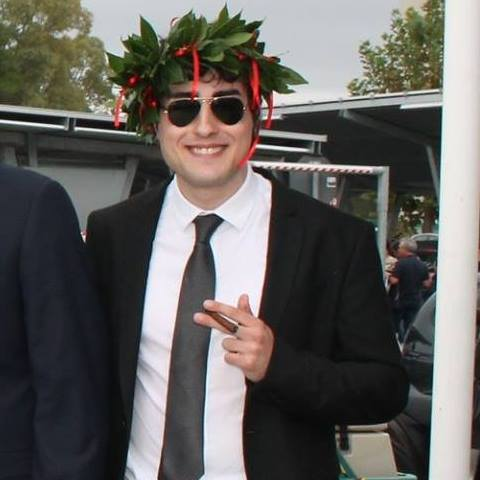
\includegraphics[width=3cm]{figures/marco.jpg}
\vspace{0.3cm}

\raisebox{-0.35ex}{
\includegraphics[width=4ex]{figures/link.png}}%
\hspace{0.05cm} /marcochiarelli

\end{figure}

%BIBLIOGRAFIA - redatta con il relativo ambiente
\begin{thebibliography}{100}
\bibitem{rif1} M. Ibbotson \emph{Cambridge English for Engineering}
\bibitem{rif2} \url{http://www.e-grammar.org/}
\end{thebibliography}

\end{document}
